% Options for packages loaded elsewhere
\PassOptionsToPackage{unicode}{hyperref}
\PassOptionsToPackage{hyphens}{url}
\PassOptionsToPackage{dvipsnames,svgnames,x11names}{xcolor}
%
\documentclass[
  12pt,
  oneside]{book}
\usepackage{amsmath,amssymb}
\usepackage{lmodern}
\usepackage{iftex}
\ifPDFTeX
  \usepackage[T1]{fontenc}
  \usepackage[utf8]{inputenc}
  \usepackage{textcomp} % provide euro and other symbols
\else % if luatex or xetex
  \usepackage{unicode-math}
  \defaultfontfeatures{Scale=MatchLowercase}
  \defaultfontfeatures[\rmfamily]{Ligatures=TeX,Scale=1}
\fi
% Use upquote if available, for straight quotes in verbatim environments
\IfFileExists{upquote.sty}{\usepackage{upquote}}{}
\IfFileExists{microtype.sty}{% use microtype if available
  \usepackage[]{microtype}
  \UseMicrotypeSet[protrusion]{basicmath} % disable protrusion for tt fonts
}{}
\makeatletter
\@ifundefined{KOMAClassName}{% if non-KOMA class
  \IfFileExists{parskip.sty}{%
    \usepackage{parskip}
  }{% else
    \setlength{\parindent}{0pt}
    \setlength{\parskip}{6pt plus 2pt minus 1pt}}
}{% if KOMA class
  \KOMAoptions{parskip=half}}
\makeatother
\usepackage{xcolor}
\usepackage{color}
\usepackage{fancyvrb}
\newcommand{\VerbBar}{|}
\newcommand{\VERB}{\Verb[commandchars=\\\{\}]}
\DefineVerbatimEnvironment{Highlighting}{Verbatim}{commandchars=\\\{\}}
% Add ',fontsize=\small' for more characters per line
\usepackage{framed}
\definecolor{shadecolor}{RGB}{248,248,248}
\newenvironment{Shaded}{\begin{snugshade}}{\end{snugshade}}
\newcommand{\AlertTok}[1]{\textcolor[rgb]{0.94,0.16,0.16}{#1}}
\newcommand{\AnnotationTok}[1]{\textcolor[rgb]{0.56,0.35,0.01}{\textbf{\textit{#1}}}}
\newcommand{\AttributeTok}[1]{\textcolor[rgb]{0.77,0.63,0.00}{#1}}
\newcommand{\BaseNTok}[1]{\textcolor[rgb]{0.00,0.00,0.81}{#1}}
\newcommand{\BuiltInTok}[1]{#1}
\newcommand{\CharTok}[1]{\textcolor[rgb]{0.31,0.60,0.02}{#1}}
\newcommand{\CommentTok}[1]{\textcolor[rgb]{0.56,0.35,0.01}{\textit{#1}}}
\newcommand{\CommentVarTok}[1]{\textcolor[rgb]{0.56,0.35,0.01}{\textbf{\textit{#1}}}}
\newcommand{\ConstantTok}[1]{\textcolor[rgb]{0.00,0.00,0.00}{#1}}
\newcommand{\ControlFlowTok}[1]{\textcolor[rgb]{0.13,0.29,0.53}{\textbf{#1}}}
\newcommand{\DataTypeTok}[1]{\textcolor[rgb]{0.13,0.29,0.53}{#1}}
\newcommand{\DecValTok}[1]{\textcolor[rgb]{0.00,0.00,0.81}{#1}}
\newcommand{\DocumentationTok}[1]{\textcolor[rgb]{0.56,0.35,0.01}{\textbf{\textit{#1}}}}
\newcommand{\ErrorTok}[1]{\textcolor[rgb]{0.64,0.00,0.00}{\textbf{#1}}}
\newcommand{\ExtensionTok}[1]{#1}
\newcommand{\FloatTok}[1]{\textcolor[rgb]{0.00,0.00,0.81}{#1}}
\newcommand{\FunctionTok}[1]{\textcolor[rgb]{0.00,0.00,0.00}{#1}}
\newcommand{\ImportTok}[1]{#1}
\newcommand{\InformationTok}[1]{\textcolor[rgb]{0.56,0.35,0.01}{\textbf{\textit{#1}}}}
\newcommand{\KeywordTok}[1]{\textcolor[rgb]{0.13,0.29,0.53}{\textbf{#1}}}
\newcommand{\NormalTok}[1]{#1}
\newcommand{\OperatorTok}[1]{\textcolor[rgb]{0.81,0.36,0.00}{\textbf{#1}}}
\newcommand{\OtherTok}[1]{\textcolor[rgb]{0.56,0.35,0.01}{#1}}
\newcommand{\PreprocessorTok}[1]{\textcolor[rgb]{0.56,0.35,0.01}{\textit{#1}}}
\newcommand{\RegionMarkerTok}[1]{#1}
\newcommand{\SpecialCharTok}[1]{\textcolor[rgb]{0.00,0.00,0.00}{#1}}
\newcommand{\SpecialStringTok}[1]{\textcolor[rgb]{0.31,0.60,0.02}{#1}}
\newcommand{\StringTok}[1]{\textcolor[rgb]{0.31,0.60,0.02}{#1}}
\newcommand{\VariableTok}[1]{\textcolor[rgb]{0.00,0.00,0.00}{#1}}
\newcommand{\VerbatimStringTok}[1]{\textcolor[rgb]{0.31,0.60,0.02}{#1}}
\newcommand{\WarningTok}[1]{\textcolor[rgb]{0.56,0.35,0.01}{\textbf{\textit{#1}}}}
\usepackage{longtable,booktabs,array}
\usepackage{calc} % for calculating minipage widths
% Correct order of tables after \paragraph or \subparagraph
\usepackage{etoolbox}
\makeatletter
\patchcmd\longtable{\par}{\if@noskipsec\mbox{}\fi\par}{}{}
\makeatother
% Allow footnotes in longtable head/foot
\IfFileExists{footnotehyper.sty}{\usepackage{footnotehyper}}{\usepackage{footnote}}
\makesavenoteenv{longtable}
\usepackage{graphicx}
\makeatletter
\def\maxwidth{\ifdim\Gin@nat@width>\linewidth\linewidth\else\Gin@nat@width\fi}
\def\maxheight{\ifdim\Gin@nat@height>\textheight\textheight\else\Gin@nat@height\fi}
\makeatother
% Scale images if necessary, so that they will not overflow the page
% margins by default, and it is still possible to overwrite the defaults
% using explicit options in \includegraphics[width, height, ...]{}
\setkeys{Gin}{width=\maxwidth,height=\maxheight,keepaspectratio}
% Set default figure placement to htbp
\makeatletter
\def\fps@figure{htbp}
\makeatother
\setlength{\emergencystretch}{3em} % prevent overfull lines
\providecommand{\tightlist}{%
  \setlength{\itemsep}{0pt}\setlength{\parskip}{0pt}}
\setcounter{secnumdepth}{5}
\usepackage{booktabs,multirow,color,eurosym}
\usepackage{amsthm}
\usepackage{multicol}
\usepackage{geometry}
\usepackage[natbibapa]{apacite}
\usepackage{lmodern} %txfonts iwona lmodern
\usepackage{hyperref}

\renewcommand{\texteuro}{\text{\euro}} 
%\hypersetup{colorlinks=false, pdfborderstyle={/S/U/W 1} }

%\geometry{executivepaper}
\geometry{a4paper}
\usepackage{makeidx}
%\usepackage{imakeidx} % Uncomment to get correct page numbers in index
\makeindex




%% Note: Pandoc (which is doing all of the output conversion behind the scenes) does not parse the content of LaTeX environments. This creates problems when you try to include LaTeX commands with curly brackets directly in your Rmd file. E.g. You can't just use `\begin{multicols}{2}` directly in your Rmd file. Luckily, a straightforward workaround is to simply define some new shortcut commands yourself as per the below.
%% See: https://stackoverflow.com/questions/25849814/rstudio-rmarkdown-both-portrait-and-landscape-layout-in-a-single-pdf/27334272#27334272
\newcommand{\btwocol}{\begin{multicols}{2}}
\newcommand{\etwocol}{\end{multicols}}


\usepackage{tikz}
\usepackage{menukeys}
\usepackage{color}
\ifLuaTeX
  \usepackage{selnolig}  % disable illegal ligatures
\fi
\usepackage[]{natbib}
\bibliographystyle{plainnat}
\IfFileExists{bookmark.sty}{\usepackage{bookmark}}{\usepackage{hyperref}}
\IfFileExists{xurl.sty}{\usepackage{xurl}}{} % add URL line breaks if available
\urlstyle{same} % disable monospaced font for URLs
\hypersetup{
  pdftitle={Quantitative Methods},
  pdfauthor={© Prof.~Dr.~Stephan Huber (Stephan.Huber@hs-fresenius.de)},
  colorlinks=true,
  linkcolor={red},
  filecolor={Maroon},
  citecolor={Blue},
  urlcolor={blue},
  pdfcreator={LaTeX via pandoc}}

\title{Quantitative Methods}
\usepackage{etoolbox}
\makeatletter
\providecommand{\subtitle}[1]{% add subtitle to \maketitle
  \apptocmd{\@title}{\par {\large #1 \par}}{}{}
}
\makeatother
\subtitle{Lecture Notes}
\author{© Prof.~Dr.~Stephan Huber (\href{mailto:Stephan.Huber@hs-fresenius.de}{\nolinkurl{Stephan.Huber@hs-fresenius.de}})}
\date{Last compiled on 17 May, 2023}

\usepackage{amsthm}
\newtheorem{theorem}{Theorem}[chapter]
\newtheorem{lemma}{Lemma}[chapter]
\newtheorem{corollary}{Corollary}[chapter]
\newtheorem{proposition}{Proposition}[chapter]
\newtheorem{conjecture}{Conjecture}[chapter]
\theoremstyle{definition}
\newtheorem{definition}{Definition}[chapter]
\theoremstyle{definition}
\newtheorem{example}{Example}[chapter]
\theoremstyle{definition}
\newtheorem{exercise}{Exercise}[chapter]
\theoremstyle{definition}
\newtheorem{hypothesis}{Hypothesis}[chapter]
\theoremstyle{remark}
\newtheorem*{remark}{Remark}
\newtheorem*{solution}{Solution}
\begin{document}
\maketitle

{
\hypersetup{linkcolor=}
\setcounter{tocdepth}{2}
\tableofcontents
}
\begin{Shaded}
\begin{Highlighting}[]
\FunctionTok{library}\NormalTok{(}\StringTok{"captioner"}\NormalTok{)}
\NormalTok{table\_nums }\OtherTok{\textless{}{-}} \FunctionTok{captioner}\NormalTok{(}\AttributeTok{prefix =} \StringTok{"Table"}\NormalTok{)}
\end{Highlighting}
\end{Shaded}

\hypertarget{preface}{%
\chapter*{Preface}\label{preface}}
\addcontentsline{toc}{chapter}{Preface}

\hypertarget{about-the-notes}{%
\section*{About the notes}\label{about-the-notes}}

\begin{itemize}
\tightlist
\item
  These notes aims to support my lecture at the HS Fresenius but are incomplete and no substitute for taking actively part in class. - A pdf version of these notes is available \href{https://raw.githubusercontent.com/hubchev/hubchev.github.io/main/qm/_main.pdf}{here}
\item
  I appreciate you reading it, and I appreciate any comments.
\item
  This is work in progress so please check for updates regularly.
\item
  Do not distribute without permission.
\end{itemize}

\hypertarget{about-the-author}{%
\section*{About the author}\label{about-the-author}}

\begin{figure}
\centering
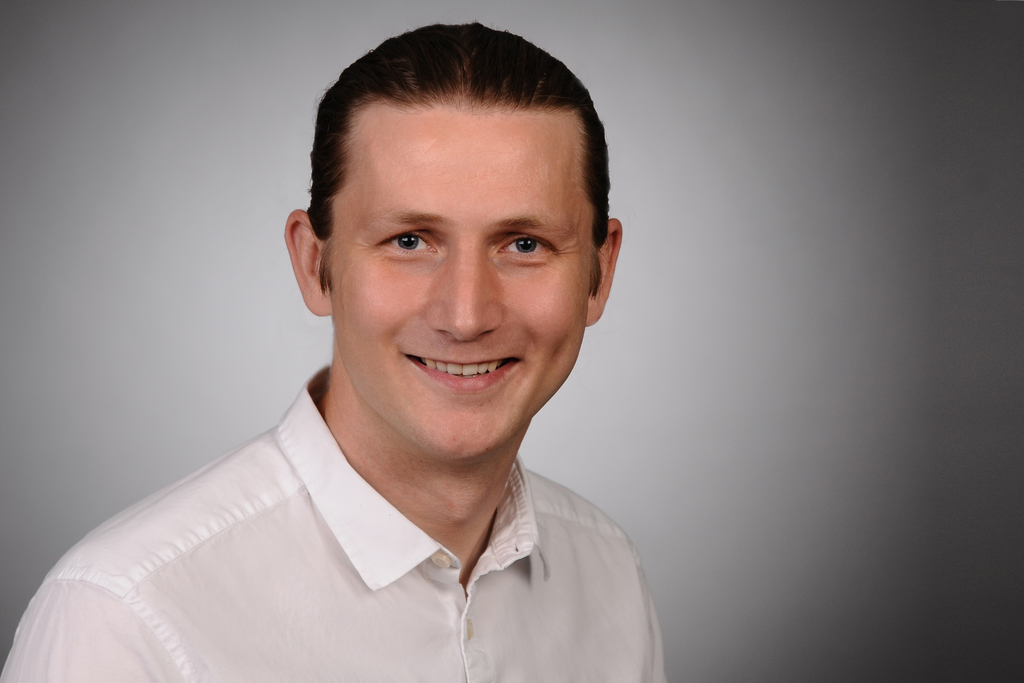
\includegraphics[width=0.25\textwidth,height=\textheight]{fig/huber2.jpeg}
\caption[\label{fig:itsme} Prof.~Dr.~Stephan Huber]{\label{fig:itsme} Prof.~Dr.~Stephan Huber\footnotemark{}}
\end{figure}
\footnotetext{Picture is taken from \url{https://sites.google.com/view/stephanhuber}}

I am a Professor of International Economics and Data Science at HS Fresenius, holding a Diploma in Economics from the University of Regensburg and a Doctoral Degree (summa cum laude) from the University of Trier. I completed postgraduate studies at the Interdisciplinary Graduate Center of Excellence at the Institute for Labor Law and Industrial Relations in the European Union (IAAEU) in Trier. Prior to my current position, I worked as a research assistant to Prof.~Dr.~Dr.~h.c. Joachim Möller at the University of Regensburg, a post-doc at the Leibniz Institute for East and Southeast European Studies (IOS) in Regensburg, and a freelancer at Charles University in Prague.

Throughout my career, I have also worked as a lecturer at various institutions, including the TU Munich, the University of Regensburg, Saarland University, and the Universities of Applied Sciences in Frankfurt and Augsburg. Additionally, I have had the opportunity to teach abroad for the University of Cordoba in Spain and the University of Perugia. My published work can be found in international journals such as the Canadian Journal of Economics and the Stata Journal. For more information on my work, please visit my private homepage at www.t1p.de/stephanhuber.

\hypertarget{contact}{%
\section*{Contact}\label{contact}}

\begin{verbatim}
   Hochschule Fresenius für Wirtschaft & Medien GmbH
   Im MediaPark 4c
   50670 Cologne
   
   Office: 4b OG-1 Bü01 (Office hour: Thursday 1-2 p.m.)
   Telefon: +49 221 973199-523
   Mail: stephan.huber@hs-fresenius.de
   Private homepage: [www.t1p.de/stephanhuber](www.t1p.de/stephanhuber)
   Github: [https://hubchev.github.io](https://hubchev.github.io)
\end{verbatim}

\hypertarget{about-this-course}{%
\section*{About this course}\label{about-this-course}}

\hypertarget{workload-of-m-ibs-8-quantitative-qualitative-methods-for-business}{%
\subsubsection*{Workload of M-IBS 8 Quantitative \& Qualitative Methods for Business}\label{workload-of-m-ibs-8-quantitative-qualitative-methods-for-business}}

125 h = 56 h (in-class) + 21 h (guided private study hours) - 48 h (private self-study).

\hypertarget{workload-of-m-ibs-8.1-quantitative-methods}{%
\subsubsection*{Workload of M-IBS 8.1 Quantitative Methods}\label{workload-of-m-ibs-8.1-quantitative-methods}}

62.5 h = 28 h (in-class) + 10.5 h (guided private study hours) - 24 h (private self-study).

\hypertarget{assessment}{%
\subsubsection*{Assessment}\label{assessment}}

Students complete this module with a written exam of 120 minutes where 50\% of the points stem from \emph{M-IBS 8.1 Quantitative Methods} and 50\% from \emph{M-IBS 8.2 Qualitative Methods}. A passing grade in this module is achieved when the overall grade is greater than or equal to 4.0.

\hypertarget{learning-outcomes}{%
\subsubsection*{Learning outcomes:}\label{learning-outcomes}}

After successful completion of the module, students are able to:

\begin{itemize}
\tightlist
\item
  assess and discuss coherent research paradigms, based on quantitative, qualitative, and mixed-methods research approaches,
\item
  explain a broad set of quantitative and qualitative methods to collect, gather, illustrate, analyze, and interpret data,
\item
  distinguish and discuss empirical strategies to identify causal mechanisms, causes, and effects.
\end{itemize}

\hypertarget{how-to-prepare-for-the-exam}{%
\subsubsection*{How to prepare for the exam:}\label{how-to-prepare-for-the-exam}}

I am convinced that reading the lecture notes, preparing for class, taking actively part in class, and trying to solve the exercises without going straight to the solutions is the best method for students to

\begin{itemize}
\tightlist
\item
  maximize leisure time and minimize the time needed to prepare for the exam, respectively,
\item
  getting long-term benefits out of the course,
\item
  improve grades, and
\item
  have more fun during lecture hours.
\end{itemize}

\hypertarget{literature}{%
\subsubsection*{Literature:}\label{literature}}

\citet{Cunningham2021Causal}, \citet{Huntington-Klein2022Effect}. \citet{Illowsky2018Introductory}. \citet{Bekes2021Data}

\hypertarget{content}{%
\subsubsection*{Content:}\label{content}}

\begin{itemize}
\item
  Research Design

  \begin{itemize}
  \tightlist
  \item
    How to Measure Socio-Economical Reality
  \item
    How to Identify Causes of Effects
  \item
    How to Identify Effects of Causes
  \item
    The Selection Problem and Ways to Solve It (Matching, Natural Experiments, Laboratory Experiments)
  \end{itemize}
\item
  Statistical Toolbox

  \begin{itemize}
  \tightlist
  \item
    Types of Data (Cross-section, Panel, Time-series, Georeferenced),
  \item
    Types of Variables (Continuous, Count, Ordinal, Categorial, Qualitative)
  \item
    Data Sampling Methods
  \item
    Descriptive Methods (Data Visualization, Statistical Moments, Correlation)
  \item
    Methods of Statistical Inference (Distribution, Statistical Tests)
  \item
    Mathematical and Statistical Software Packages (R, SPSS, Excel, WolframAlpha, etc.)
  \end{itemize}
\item
  Methods

  \begin{itemize}
  \tightlist
  \item
    Data Mining (Graphical Visualizations, Cluster Analysis, Factor Analysis)
  \item
    Regression Analysis (Matching, Instrument Variables, Difference in Difference, Fixed Effects, Regression Discontinuity)
  \item
    Other Methods (Time Series Analysis, Spatial Analysis, Simulations, Qualitative Comparative Analysis, etc.)
  \end{itemize}
\end{itemize}

\hypertarget{about-how-to-learn-and-prepare-for-the-exam}{%
\subsubsection*{About how to learn (and prepare for the exam)}\label{about-how-to-learn-and-prepare-for-the-exam}}

\begin{figure}
\centering
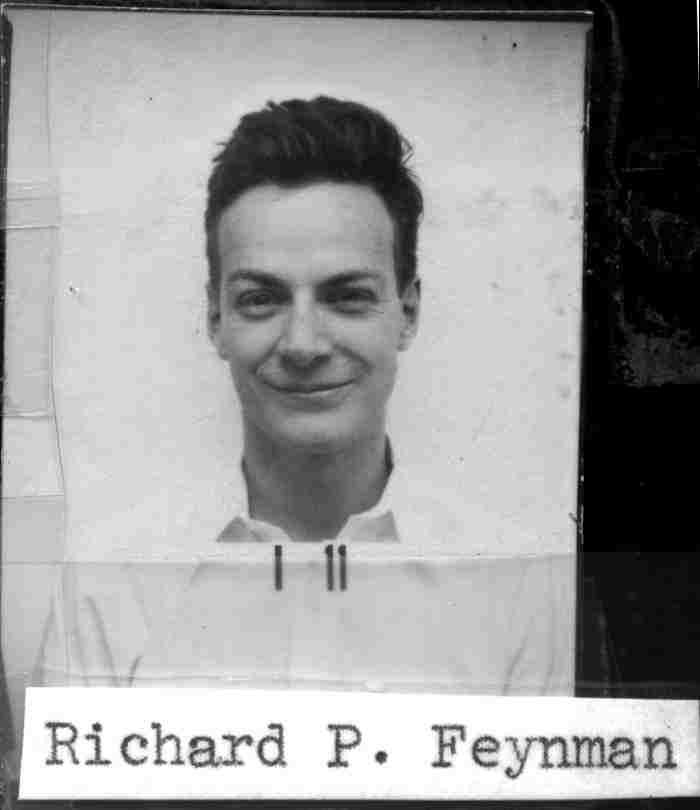
\includegraphics[width=0.25\textwidth,height=\textheight]{fig/Richard-Feynman.jpg}
\caption[\label{fig:feynman} Richard P. Feynman's badge photo from Los Alamos National Laboratory]{\label{fig:feynman} Richard P. Feynman's badge photo from Los Alamos National Laboratory\footnotemark{}}
\end{figure}
\footnotetext{Picture is taken from \url{https://repository.aip.org/islandora/object/nbla\%3A299600}}

Richard P. Feynman:

\begin{quote}
``I don't know what's the matter with people: they don't learn by understanding; they learn by some other way ­ by rote, or something. Their knowledge is so fragile!''
\end{quote}

Stephan Huber:

\begin{quote}
``I agree with Feynman: The key to learning is understanding. However, I believe that there is no understanding without practice, that is, solving problems and exercises by yourself with a pencil and a blank sheet of paper without knowing the solution in advance.''
\end{quote}

\begin{itemize}
\tightlist
\item
  Study the lecture notes, i.e., try to understand the exercises and solve them yourself.
\item
  Study the exercises, i.e., try to understand the logical rules and solve the problems yourself.
\item
  Test yourself with past exams that you will find on ILIAS. The structure of the exam is more or less the same every semester.
\item
  If you have the opportunity to form a group of students to study and prepare for the exam, make use of it. It is great to help each other, and it is very motivating to see that everyone has problems sometimes.
\item
  If you have difficulties with some exercises and the solutions shown do not solve your problem, ask a classmate or contact me. I will do my best to help.
\end{itemize}

\hypertarget{personal-note}{%
\section*{Personal note}\label{personal-note}}

Dear students,

If the title of this course ``Quantitative \& Qualitative Methods for Business'' seems uninteresting to you, I assure you that it is actually quite exciting because it focuses on how we can use information to understand how the world and business works and how to interpret facts. The course will enhance your data literacy, help you think critically, and improve your personal decision-making skills.

One way we can do this is by understanding the differences between quantitative and qualitative data and how they can be used to inform our choices.

Quantitative data is information that can be measured, such as numbers and statistics, while qualitative data is information that cannot be measured and is often expressed in words or other non-numerical forms.

Both forms of information are crucial for making good decisions. Without sufficient information, it can be difficult to evaluate the options and potential outcomes of a decision, leading to poor or uninformed choices. In general, the more information a decision-maker has and the faster and better the information can be used, the better they will be to make a sound decision.

The methods we discuss in this course will help you systematically gather information and make sense of it.

Enjoy the course!

\hypertarget{doing-research}{%
\chapter{Doing research}\label{doing-research}}

\begin{figure}
\centering
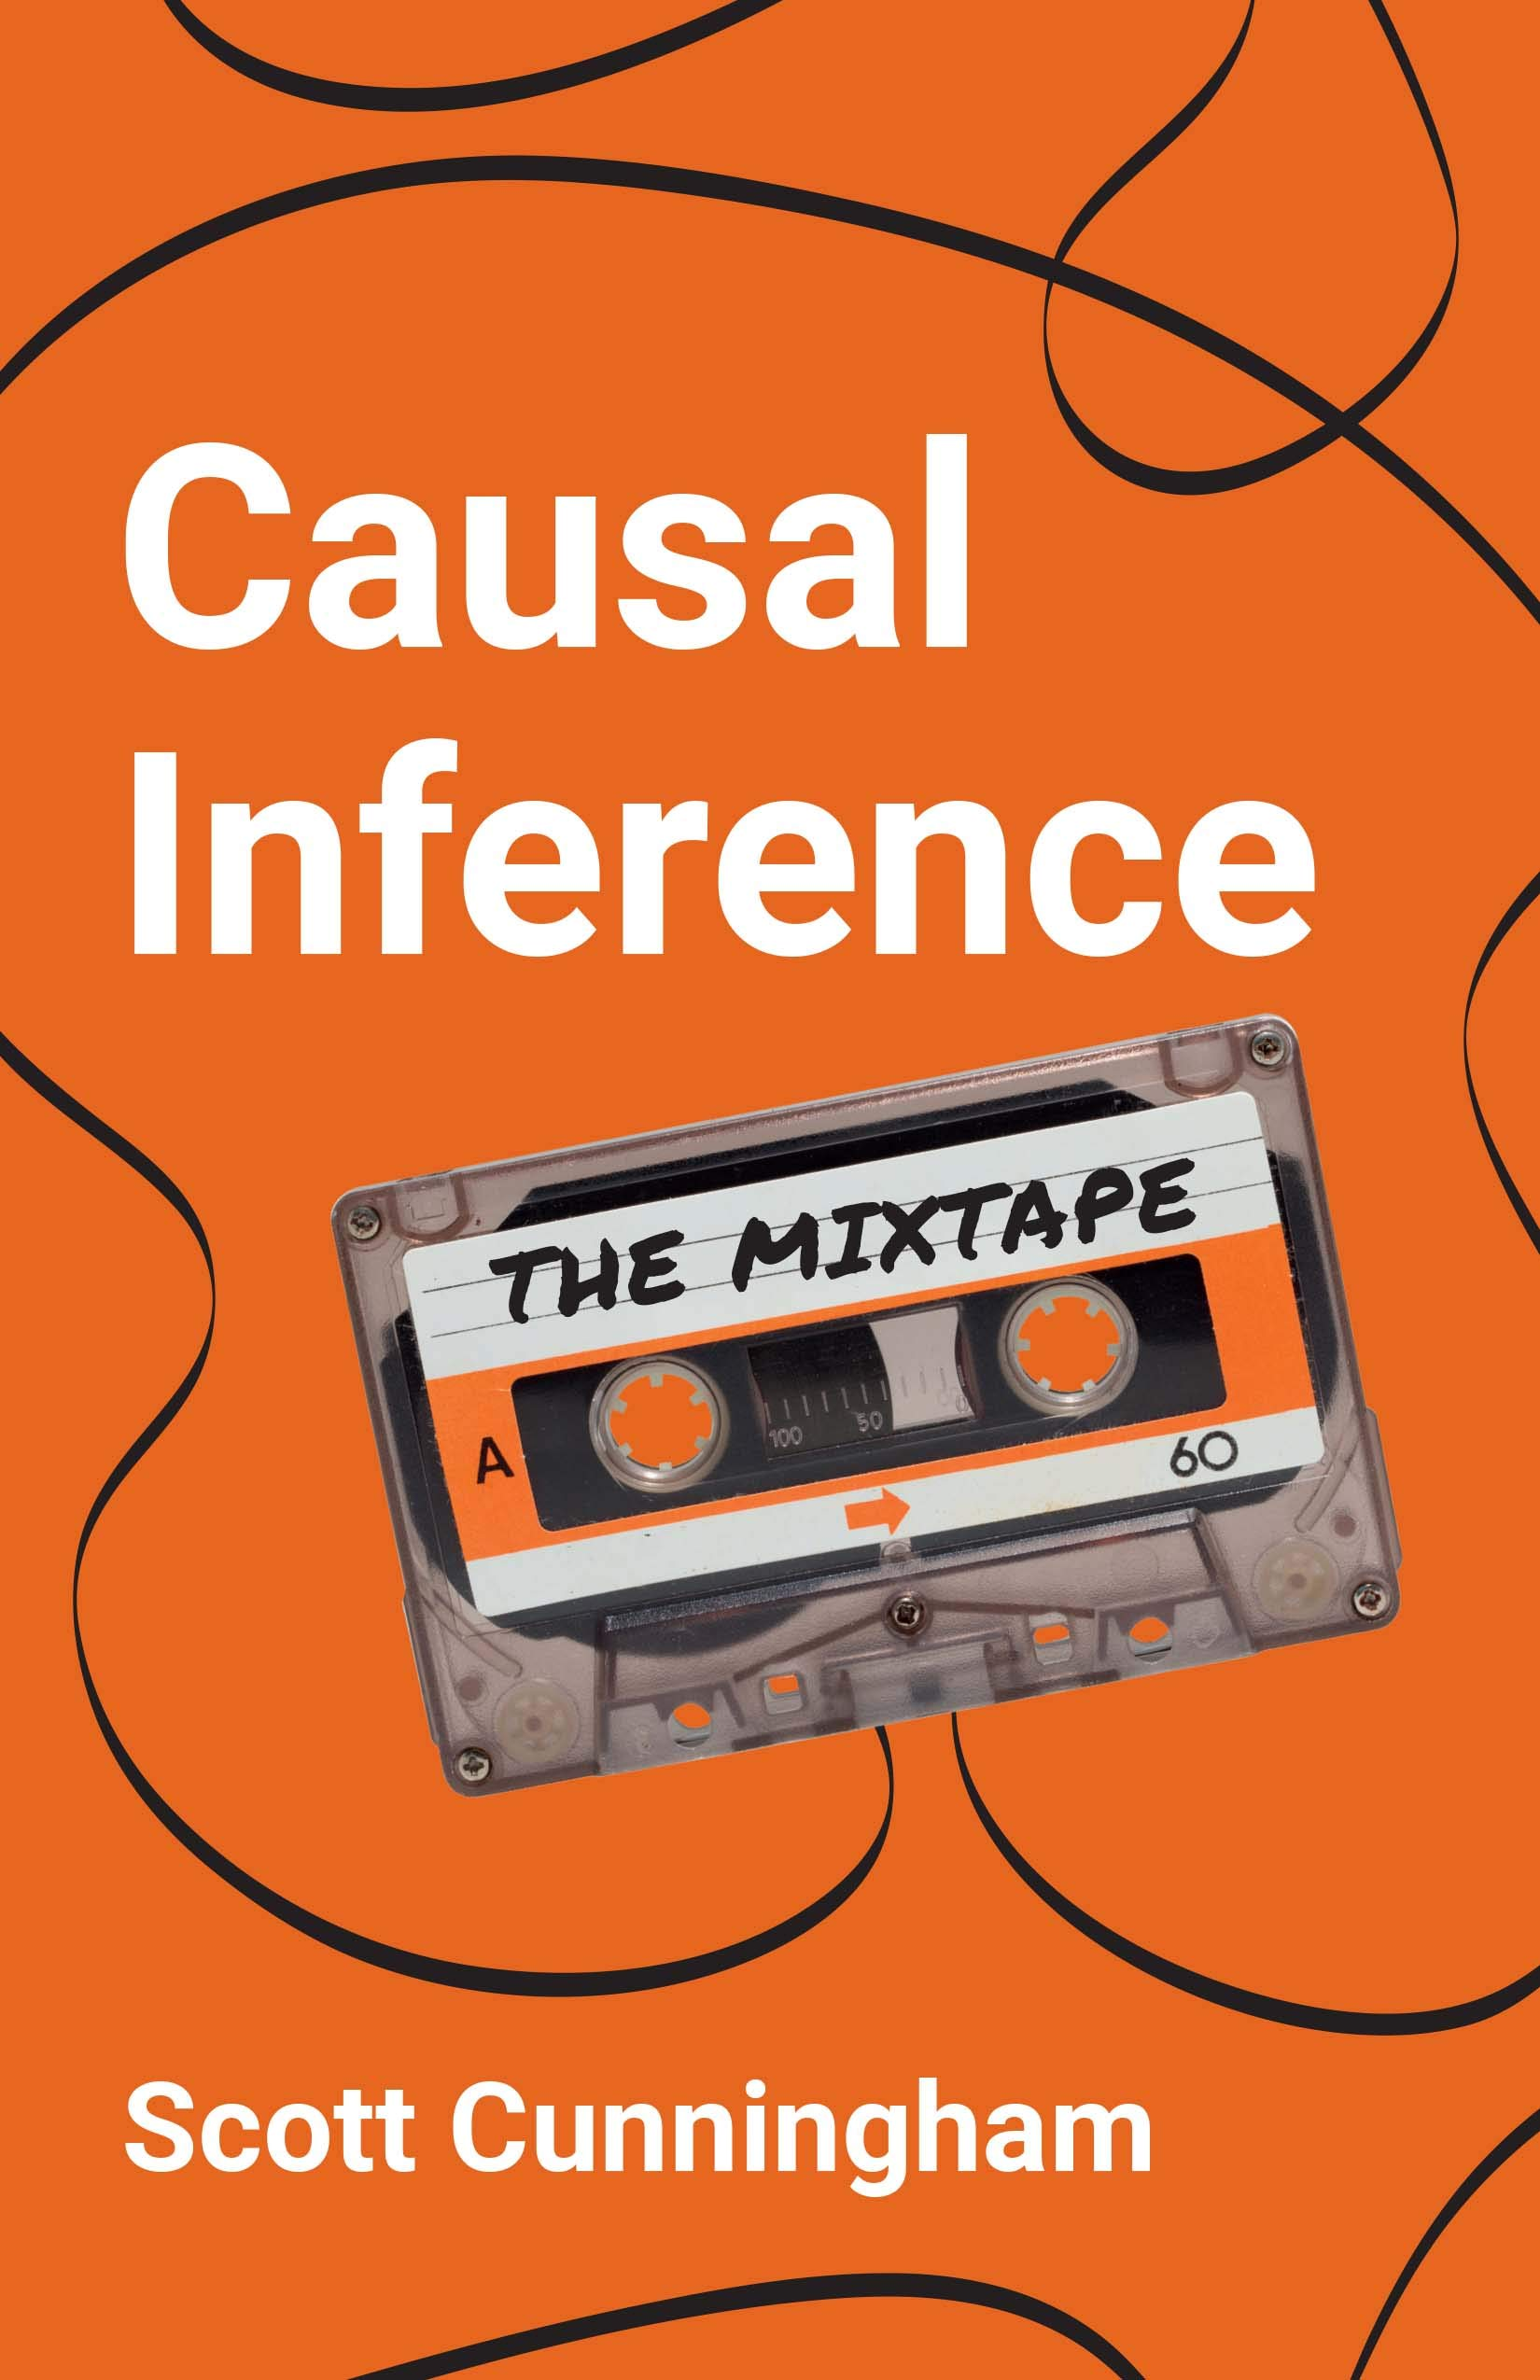
\includegraphics[width=0.25\textwidth,height=\textheight]{fig/cover-ci.jpg}
\caption{\label{fig:ci-book} Causal Inference: The Mixtape. A textbook by Scott \citet{Cunningham2021Causal}.}
\end{figure}

\begin{quote}
\emph{``True scientists do not collect evidence in order to prove what they want to be true or what others want to believe. That is a form of deception and manipulation called propaganda, and propaganda is not science. Rather, scientific methodologies are devices for forming a particular kind of belief. Scientific methodologies allow us to accept unexpected, and sometimes undesirable, answers.''} \citep[p.~10]{Cunningham2021Causal}
\end{quote}

\hypertarget{everybody-can-do-research}{%
\section{Everybody can do research}\label{everybody-can-do-research}}

Research often involves exploring unknown territory and seeking out new information through methods such as attending conferences, conducting interviews and experiments, and reading related research. This process can lead to the discovery of valuable techniques or insights that address important issues in society or science.

\begin{figure}
\centering
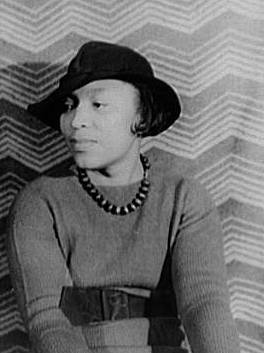
\includegraphics[width=0.2\textwidth,height=\textheight]{fig/Zora_Neale_Hurston.jpg}
\caption[\label{fig:hurston} Zora Neale Hurston, 1891-1960]{\label{fig:hurston} Zora Neale Hurston, 1891-1960\footnotemark{}}
\end{figure}
\footnotetext{Photography is taken from Library of Congress: Prints \& Photographs Division, Carl van Vechten Collection, Reproduction Number LC-USZ62-54231, see: \url{https://www.loc.gov/pictures/item/2004663047/}..}

\begin{quote}
\emph{``Research is formalized curiosity. It is poking and prying with a purpose.''} \citep{Hurston2010Dust}
\end{quote}

Before I go into how empirical research can and should be conducted, I would like to assert that each of us is a researcher in some sense and that you don't need a degree or a higher education to be a (good) researcher. Each of my four children (ages 2, 5, 6, and 8), for example, explores the world and learns something new every day. Even though none of my children is yet able to verify the novelty of their acquired knowledge and write it down in scientific form, I will claim that mine, like practically all children, are already little scientists. Why? Well, they explore unknown territory and search for information to discover new techniques that will make their lives pleasant. Of course, they don't attend conferences or read journals to do this. They have never heard terms such as ontology, epistemology, axiology, or quantitative and qualitative methods. They are using methods that they have mastered for their age. They interview me, my wife and all other people around and they conduct experiments. For example, all my children liked to throw plates, cutlery, cups and alike from the table when they were about one year old. At first the throwing was just an accident, but they quickly found out that each throw was followed by a sound when the object touched the stone floor. My first son, in particular, took great delight in making these sounds. He threw everything within reach to the ground and giggled with joy at the clink he made when the object hit the ground. Perhaps he was also enjoying the attention he was getting from us parents through these actions. In any case, the behavior annoyed us. Wiping food scraps off the floor is not a nice thing to do. Unfortunately, at that time my son did not accept any argument to refrain from throwing. Neither a stern look nor a definite ``no'' helped to stop this behavior. Too great was the joy at the relationship he had figured out, which was, ``I throw something off the table and it always clangs beautifully loud.'' So I started to do some research to figure out what I could do to stop him. The short answer I found can be summed up pretty well as ``nothing''. There is practically no good method to change the behavior without possibly negatively influencing his early childhood development. The reason is he did some research and we should not suppress that. Besides nature and material research he did social research: He found out that things fall to the ground (gravity), that things break and make different sounds (material research), and that other people notice him when he throws things (social research).

\begin{figure}
\centering
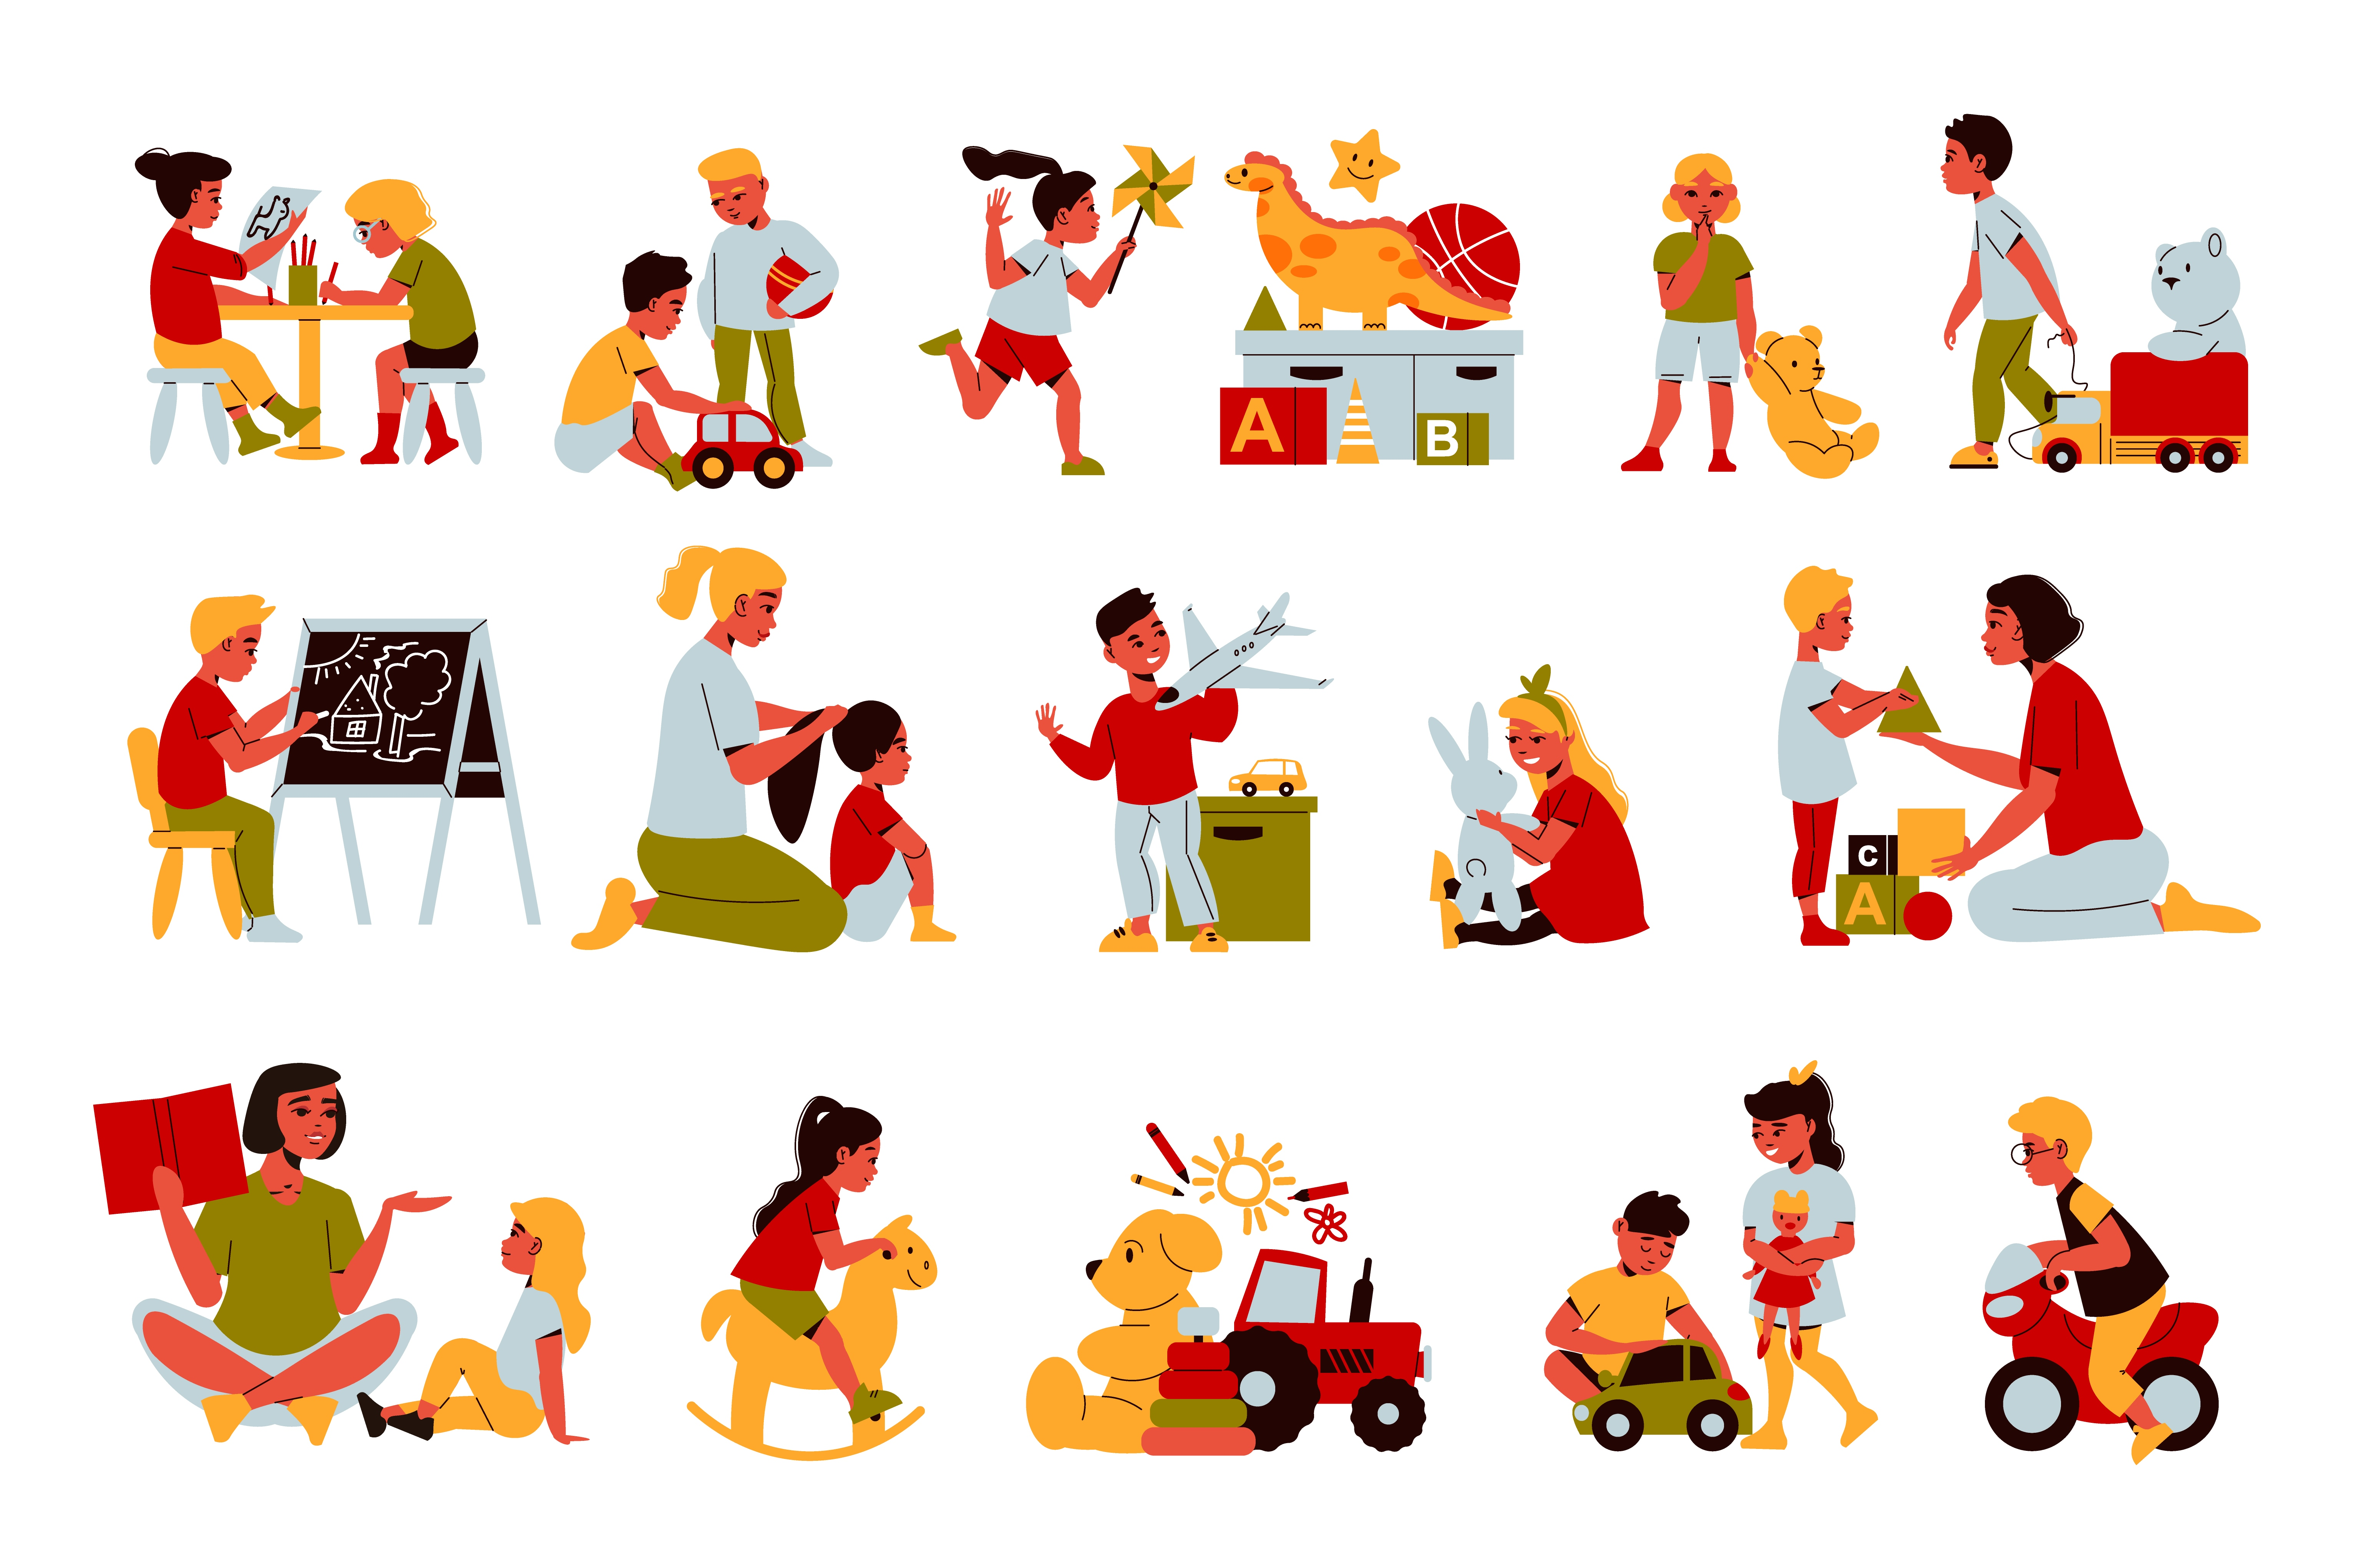
\includegraphics[width=0.75\textwidth,height=\textheight]{fig/2101.i605.022.P.m005.c25.kindergarten set.jpg}
\caption[\label{fig:children} Children as little researcher]{\label{fig:children} Children as little researcher\footnotemark{}}
\end{figure}
\footnotetext{Image by macrovector on Freepik, see: \url{https://www.freepik.com/free-vector/kindergarten-set-isolated-icons-with-toys-characters-kids-practicing-with-teacher-playing-games-vector-illustration_26760074.htm}}

Once, when we were eating at a friend's house, my son (once again) threw everything off the table one after the other in unobserved moments. This time, however, it made no noise. The carpet under the table muffled everything. My son was irritated and at some point became really angry. Why? Well, his surely believed reality and his law ``I throw something from the table and then it always clangs beautifully loud.'' was falsified. Soon he understood that his law only had to be adapted a little. It was then: ``I throw something from the table and it clangs then beautifully loudly if a stone floor is under me.'' He repeated his experiments for a few more weeks, to check its validity. In the meantime he does other experiments trying to contribute to his own knowledge.

In general, the purpose of research is to find new knowledge or discover new ways to use existing knowledge in a creative way so as to generate new concepts, methodologies, inventions and understandings that -now or later- may be of some value for the human mankind. In simple terms, we aim to find something out. We aim to find a new law, a new relationship, a new insight. Or, we aim to challenge and revise existing insights on how the world works. You don't need a degree to do that.
All you need is interest, open-mindedness, and a willingness to revise your ideas about how the world works. The latter is perhaps the most important skill you need to be a good researcher. Otherwise, one is a narrow-minded, and bigoted person who is too proud to follow up an insight with a change of mind.

I myself have a quick and happy tendency to change my views because it is a statement of a fresh understanding. Here are two more quotes from historically more significant people than me that are along the same lines and should convince you that changing your mind is not a sign of weakness, but of strength. Especially in science, the willingness to change one's mind is essential.

\begin{figure}
\centering
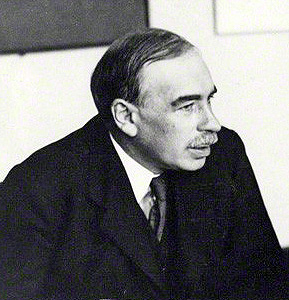
\includegraphics[width=0.2\textwidth,height=\textheight]{fig/Keynes_1933.jpg}
\caption[\label{fig:keynes} John Maynard Keynes (1883-1946)]{\label{fig:keynes} John Maynard Keynes (1883-1946)\footnotemark{}}
\end{figure}
\footnotetext{Photography is public domain and stems from \url{https://de.wikipedia.org/wiki/John_Maynard_Keynes\#/media/Datei:Keynes_1933.jpg}}

\begin{quote}
\emph{``When the facts change, I change my mind. What do you do, sir?''}\footnote{This quote is often attributed to Keynes, but there is no clear evidence for it, see: \url{https://quoteinvestigator.com/2011/07/22/keynes-change-mind/}}
\end{quote}

\begin{figure}
\centering
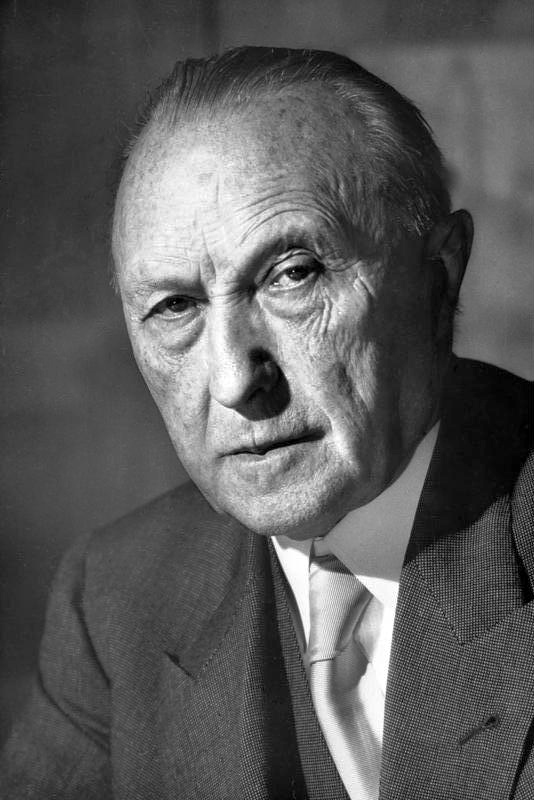
\includegraphics[width=0.15\textwidth,height=\textheight]{fig/Bundesarchiv_B_145_Bild-F078072-0004,_Konrad_Adenauer.jpg}
\caption[\label{fig:adenauer} Konrad Adenauer (1876-1967)]{\label{fig:adenauer} Konrad Adenauer (1876-1967)\footnotemark{}}
\end{figure}
\footnotetext{This photography from 1952 is public domain and stems from the Bundesarchiv, B 145 Bild-F078072-0004, Katherine Young, CC BY-SA 3.0 DE.}

\begin{quote}
\emph{``What do I care about the rubbish I said yesterday? No one can stop me from getting smarter every day.''} (``Was interessiert mich mein Geschwätz von gestern? \ldots{} es kann mich doch niemand daran hindern, jeden Tag klüger zu werden.'')\footnote{Freely quoted (and translated) from \citet[p.~521]{Weymar1955Konrad}}
\end{quote}

\hypertarget{its-difficult-to-do-good-research}{%
\section{It's difficult to do good research}\label{its-difficult-to-do-good-research}}

Simply trying something and seeing what happens, like my children do, is a research method that relies on luck and chance. Before I go into more grown-up ways of doing research, I want to emphasize that the role of chance and serendipity in research is often downplayed and not acknowledged. The most well-known example of such research is the discovery of penicillin by Alexander Fleming. In 1928, Fleming was studying the properties of staphylococcus bacteria when he noticed that a mold called Penicillium notatum had contaminated one of his bacterial cultures. He noticed that the mold seemed to be inhibiting the growth of the bacteria, and he began to investigate this further. Eventually, he was able to isolate and purify the active ingredient in the mold, which he named penicillin, and he discovered that it had powerful antibiotic properties. This discovery revolutionized the field of medicine and has saved countless lives.

\begin{figure}
\centering
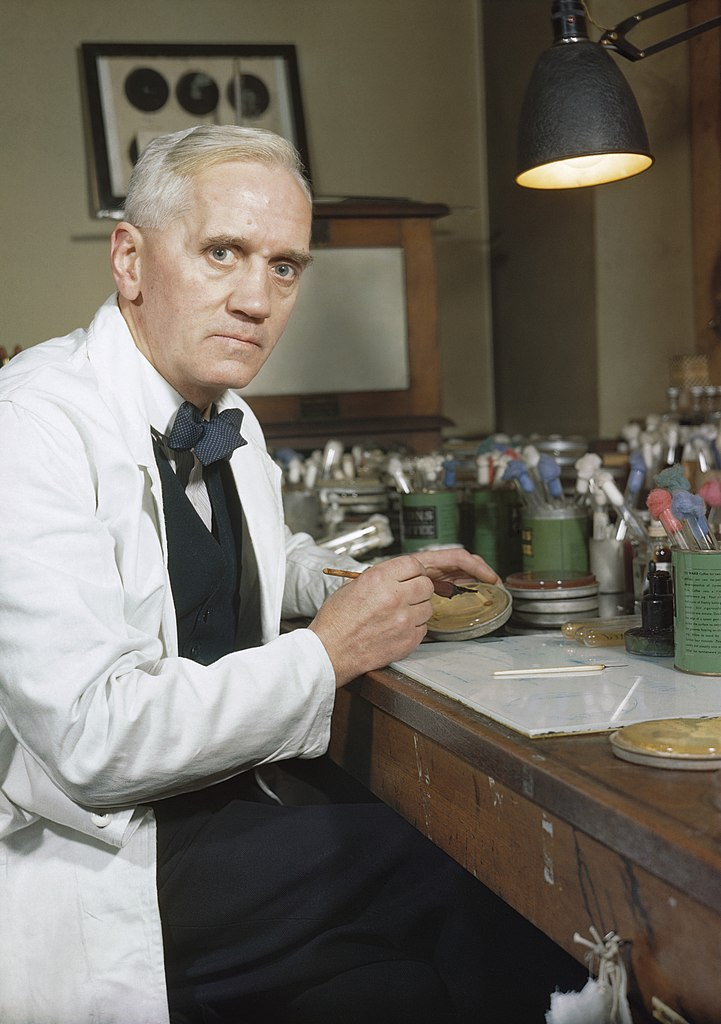
\includegraphics[width=0.2\textwidth,height=\textheight]{fig/Synthetic_Production_of_Penicillin_TR1468.jpg}
\caption[\label{fig:fleming} Sir Alexander Fleming (1881-1955)]{\label{fig:fleming} Sir Alexander Fleming (1881-1955)\footnotemark{}}
\end{figure}
\footnotetext{Photography is public domain and stems from \url{https://en.wikipedia.org/wiki/File:Synthetic_Production_of_Penicillin_TR1468.jpg}}

Doing something on purpose and observing how things respond to the action can be considered a research strategy. Acting like a child or just waiting for something to happen by chance can also be considered a research strategy, and of course this can contribute greatly to knowledge. However, it are a naïve and poorly targeted strategies to conduct research. There are more grown-up research methods that are targeting more precisely the gaps in our knowledge and speed up innovation in the field where progress is desperately needed.

What we do and how we observe what is happening should be done in a way to increase the likeliness that we find something new and interesting and in a way that allows us to be rather certain that our results are true and are less likely to be falsified soon later.

For example, assume that there is a disease that can kill people. The childish way to figure out how to cure the disease would be to observe who gets sick and who dies, and finally hope to find a cure for the disease by accidental observation. This is most likely not a very promising and quick method. It would probably be much better to study the matter systematically. For example, a laboratory should first seek to isolate the causative virus or bacterium in order to be able to grow and study it outside the danger to humans. Once this is done, we need a precise plan on how we can use all the available knowledge to cure the disease, protect people from infection, or help them survive the disease. In short, we need a strategic way to conduct research, i.e., a research strategy or design.

A \emph{research strategy} is a general plan for conducting a study and a \emph{research design} is a detailed plan for conducting the study. These words are frequently used interchangeably.
A research strategy depends on many things including the question, the resources available, the current state of knowledge, the ambitions, whether quantitative or quantitative data are used, and what is considered to be the criteria of good research.

Before discussing some research strategies that can provide reasonable answers to certain types of questions, we should clarify how to ask a research question and what qualifies a research question.

\hypertarget{asking-questions-lika-a-good-researcher}{%
\section{Asking questions lika a good researcher}\label{asking-questions-lika-a-good-researcher}}

Unfortunately, there is no one research strategy that is appropriate for all questions and, what is worse, there is still controversy about what constitutes good research and how to properly ask a research question. In particular, this controversy takes place between researchers who use quantitative data and statistical methods and researchers who use qualitative data and methods.

Quantitative researchers are more interested in determining the causes of effects using experiments with measurable results, and they attempt to quantify the effects of causes.
Qualitative researchers also try to determine the causes of effects . However, their data analysis does rely less on statistical inference. A qualitative data set not necessarily requires (large) random samples or structured data (all the data that you can structure in a spreadsheet) in general, but allows to analyze selective and unstructured data (that is data in form of audio, video, text, images and alike). Qualitative research methods allow to classify these data into patterns or to interpret them in a meaningful way in order to arrive at results.
Qualitative researchers are more concerned with the \emph{why and how} of decision making and examine people's behavior, beliefs, perceptions of events, experiences, attitudes, interactions, and more in great depth.

In empirical research, inductive and deductive are two different approaches to reasoning. \emph{Inductive reasoning} is a process of collecting data from various sources, such as interviews, surveys or observations, and then use this data to identify patterns, themes, or relationships that can form the basis of a new hypothesis or theory. The goal of these exploratory studies, is to generate new ideas or insights about a topic, rather than testing a specific hypothesis.
\emph{Deductive reasoning} is a process in which the researcher starts with a general theory or hypothesis with the goal to test a specific hypothesis or theory. In most cases, a combination of both inductive and deductive reasoning may be used to formulate the research question and to design the empirical identification strategy.

In what follows, however, we focus on the criteria for \emph{good research} that are more commonly used in evaluating the quality of quantitative research.

\begin{exercise}
\protect\hypertarget{exr:effect1u2}{}\label{exr:effect1u2}The Effect ch.1+2

Read chapter 1 and 2 of \citet{Huntington-Klein2022Effect} and answer the questions below. The book is freely available at \url{https://theeffectbook.net} and here is the link to chapter 1: \url{https://theeffectbook.net/ch-TheDesignofResearch.html}

\begin{figure}
\centering
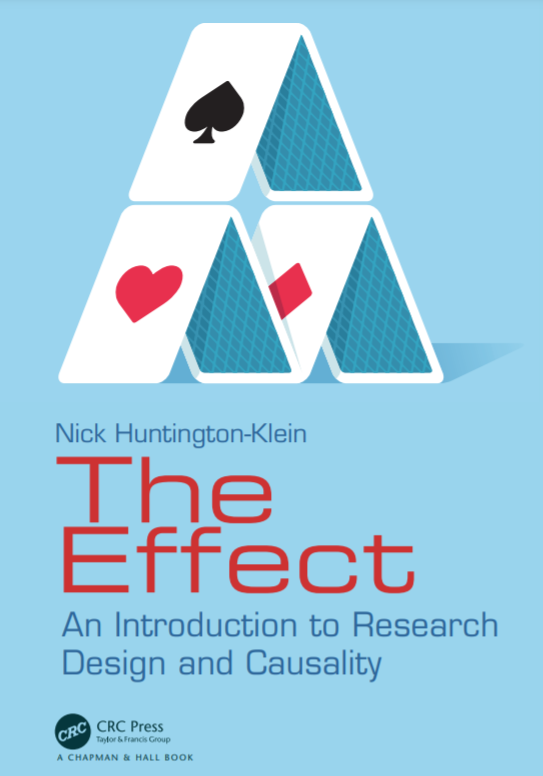
\includegraphics[width=0.25\textwidth,height=\textheight]{fig/cover-effect.png}
\caption{\label{fig:theeffect} The book \emph{The Effect: An Introduction to Research Design and Causality} by Nick \citet{Huntington-Klein2022Effect}.}
\end{figure}

\begin{enumerate}
\def\labelenumi{\arabic{enumi}.}
\tightlist
\item
  What is the main focus of the book the author is writing about?

  \begin{enumerate}
  \def\labelenumii{\alph{enumii})}
  \tightlist
  \item
    Philosophy of science
  \item
    Qualitative research methods
  \item
    Empirical research and quantitative methods to identify and measure causal effects
  \item
    Statistics
  \end{enumerate}
\item
  What is the main challenge faced by quantitative empirical research, according to the author?

  \begin{enumerate}
  \def\labelenumii{\alph{enumii})}
  \tightlist
  \item
    Difficulty in obtaining accurate measurements
  \item
    Difficulty in interpreting measurements
  \item
    Difficulty in obtaining data that allows to answers the research question
  \item
    Difficulty in designing a research that gets a lot of attention
  \end{enumerate}
\item
  What is the author's main point about research questions?

  \begin{enumerate}
  \def\labelenumii{\alph{enumii})}
  \tightlist
  \item
    They should be well-defined, answerable, and understandable
  \item
    They should be simple and easy to answer
  \item
    They should be related to the world of traffic
  \item
    They should be related to the field of quantum mechanics
  \end{enumerate}
\end{enumerate}

Please find solution to the exercise \protect\hyperlink{sol:effect1u2}{in the appendix.}
\end{exercise}

\hypertarget{features-of-good-research}{%
\section{Features of good research}\label{features-of-good-research}}

In order to make you a competent researcher who does not have to wait for a lucky chance but has a clear strategy, let's discuss the criteria of a good research. Before I do that, however, I must make a disclaimer: there is a lack of consensus on what constitutes high-quality research in social sciences. In my experience, the practical benefits of such a tedious discussion are quite small. All I like to put forward is that I believe that all social science disciplines such as sociology, anthropology, psychology, economics, business administration, and education using quantitative methods agree that good research should be replicable, reproducible, transparent, reliable, and valid.

\hypertarget{reliability-and-validity}{%
\subsection{Reliability and validity}\label{reliability-and-validity}}

A research design is a plan to examine information in a systematic and controlled way so that the results of the research are \emph{valid and reliable}.

\emph{Validity} refers to the accuracy and truthfulness of research findings. In other words, if a study is valid, it should measure what it is intended to measure and produce results that are representative of the population being studied. Validity is important because it helps to ensure that the conclusions drawn from a study are supported by the data and are not based on flawed or biased methods.

\emph{Reliability} refers to the consistency and stability of research findings. In other words, if a study is reliable, it should produce similar results if it is repeated using the same methods and conditions. Reliability is important because it helps to ensure that the results of a study are not simply due to chance or random error.

Both reliability and validity are important considerations in research, and researchers strive to maximize both in their studies. However, it is important to note that it is often difficult to achieve both at the same time, and trade-offs may need to be made between the two.

\textbf{Statement}: A good research design should aim to minimize bias and maximize the reliability and validity of the research. It should also be appropriate for the research question being asked and the resources available to the researcher.

\hypertarget{high-reliability-and-low-validity}{%
\subsubsection*{High reliability and low validity}\label{high-reliability-and-low-validity}}

An example of a study that has high reliability but low validity is a study that measures the weight of a group of people using a digital scale. If the scale is consistently accurate and produces the same weight measurements each time it is used, then the study has high reliability. However, if the scale is not calibrated correctly and produces inaccurate weight measurements, then the study has low validity.

Another example of a research design that has high reliability but low validity is a study that uses a highly reliable measurement tool, such as a standardized test, to measure a concept that is not directly related to the research question being asked. For example, a study that uses a standardized math test to measure students' critical thinking skills may have high reliability because the test is consistently accurate and produces similar scores each time it is administered. However, the study may have low validity because the math test is not an appropriate tool for measuring critical thinking skills. As a result, the results of the study may not be representative of the students' true critical thinking abilities.

\hypertarget{high-validity-and-low-reliability}{%
\subsubsection*{High validity and low reliability}\label{high-validity-and-low-reliability}}

An example of a study that has high validity but low reliability is a study that asks people to self-report their eating habits. While the study may produce accurate and representative results about people's eating habits, the self-reported data may vary from person to person and may not be consistent over time. As a result, the study has high validity but low reliability.

Another example of a study that has high validity but low reliability is a study that uses a highly valid measurement tool, such as a survey, to measure a concept that is directly related to the research question being asked. However, the study may have low reliability because the survey is not administered consistently or the responses are not accurately recorded. For example, a study that uses a survey to measure students' attitudes towards school may have high validity because the survey is relevant to the research question and accurately measures the students' attitudes. However, if the survey is not administered consistently or the responses are not accurately recorded, the study may have low reliability. As a result, the results of the study may not be representative of the students' true attitudes towards school.

\hypertarget{trade-offs-between-reliability-and-validity}{%
\subsubsection*{Trade-offs between reliability and validity}\label{trade-offs-between-reliability-and-validity}}

In research design, trade-offs may need to be made between reliability and validity. For example, a study that uses a highly reliable measurement tool may not be valid if the tool is not appropriate for the research question being asked. Similarly, a study that uses a highly valid measurement tool may not be reliable if the tool is prone to producing inconsistent results. As a result, researchers must carefully consider both reliability and validity when designing a study and make trade-offs as necessary to maximize the overall quality of the research.

\hypertarget{generalizability}{%
\subsection{Generalizability}\label{generalizability}}

Coming back to my little son who threw everything within reach to the ground and giggled with joy at the clink he made when the object hit the ground. He identified a cause-and-effect relationship through an experiment in an controlled environment. His law ``I throw something off the table and it always clangs'' worked in our home. To our regret, it was replicateable and he really tried hard to falsify it. Moreover, his study was reasonable valid as his study design, conduct, and analysis could answer his research questions without bias (at least ignoring the other noises that his sibling and parents make coincidentally during his experiment). Scientist call this \emph{internal validity}.
However, he also found out that when he leaves our home, things are sometimes a bit different, for example, if there is a carpet under the table. Thus, his insights from our home findings can't be generalized to other contexts, at least not without further specifications. Scientist call this \emph{external validity}.

\textbf{Statement}: Internal validity examines whether the study design, conduct, and analysis answer the research questions without bias. External validity examines whether the study findings can be generalized to other contexts.

\hypertarget{replicability-reproducibility-transparency-and-other-criteria}{%
\subsection{Replicability, reproducibility, transparency, and other criteria}\label{replicability-reproducibility-transparency-and-other-criteria}}

It must be possible to repeat the research conducted for several reasons. For example, if you can repeat a study with slightly changed parameters, you are able to improve its external validity and show that the conclusions drawn are reliable. To be able to repeat a study, everything that is important for drawing a conclusion from the research has to be mentioned. This is what we call \emph{transparency}. Moreover, everything in the study must have been done in such a way that we can check the results for truth. In the best case, it is possible to \emph{reproduce} the results in the same way they were obtained in the study. Sometimes this is not possible because, for example, we can never really ask the same people again in a survey, and even if we found the same people, they would have gotten older and not be the same people as before. In such a case, it should at least be possible to \emph{replicate} the research. This means that we can basically do the same thing in a setting that differs only in those things that we cannot avoid to be different. For example, by interviewing a group of people who match the people in the study to replicate them on all the important characteristics like age.

In an empirical quantitative research study, for example, the data and the code written to process the data and analyze it should be accessible to everyone.

In a qualitative study, all sources of information should be stated, and the circumstances leading to a conclusion should be fully explained. For example, all transcripts of interviews conducted should be made available. The researcher should provide rich and detailed descriptions of the data and the context in which it was collected. Research should be provided with rich, nuanced, and multi-layered accounts of social phenomena by describing and interpreting the meanings, beliefs, and practices of the people being studied. That is known as \emph{thick description}. Researchers typically employ a variety of methods such as participant observation, in-depth interviews, and document analysis, and they often use multiple sources of data to triangulate their findings. The goal is to provide a holistic and broad understanding of the phenomenon being studied, rather than a narrow view from the researcher's perspective.

There are some other criteria of good research that are worth mentioning:

\hypertarget{credibility}{%
\subsubsection*{Credibility}\label{credibility}}

The research should be trustworthy and believable, and the researcher should provide detailed descriptions of the methods used to ensure transparency.

\hypertarget{reflective-practice}{%
\subsubsection*{Reflective Practice}\label{reflective-practice}}

The researcher should engage in reflexive practice throughout the research process, which means to be critically aware of oneself, one's own assumptions, and one's own role in the research process.

\hypertarget{triangulation}{%
\subsubsection*{Triangulation}\label{triangulation}}

The researcher should use multiple methods, sources, and perspectives to increase the credibility of the findings (also see \emph{thick description} above).

\hypertarget{transferability}{%
\subsubsection*{Transferability}\label{transferability}}

The conclusions drawn from looking at mostly unstructured data in qualitative research can hardly be generalized in a strict sense, as they depend crucially on the context of the object of study. For example, generalizability is essentially impossible in a qualitative case study, since everything depends on the specific situation of an individual, a company, or a group of people considered in the specific setting. This means that in a case study or interview, we may be looking at only a few or even a single observation that cannot be considered \emph{representative} of the larger population, as generalizability does. Transferability, on the other hand, gives the reader the ability to transfer the findings into other contexts. The ability to transfer contextual findings to other cases is a goal of qualitative research, and the author of a study should attempt to offer the information in a way that allows the reader to transfer the findings to the setting or situation with which he or she is familiar.

\hypertarget{the-role-of-resources-data-and-ethics}{%
\section{The role of resources, data and ethics}\label{the-role-of-resources-data-and-ethics}}

There are several types of research designs, including experimental designs, quasi-experimental designs, and observational designs. Each of these designs took advantage of various empirical methods and statistical procedures. We will discuss some of them later on. The choice of research design, of course, should depend on the research question being asked, the resources available, and the type of data that is being collected. The research design should also take into account any ethical considerations that may be relevant to the research.
The research design should be chosen so that it is well suited to answer the research question. For example, if one is interested in the question ``Why do some people get sick with a certain disease and others do not?'' then an observational study design to determine possible \emph{causes of effect} may be appropriate. These identified potential causes should then be verified followed by an experimental study. Relatively, a statistical analysis should be used which would allow the \emph{effects of causes} to be evaluated. The aim should be to identify necessary and sufficient circumstances to develop a disease. Also circumstances should be described that favor a disease.

If the question is a ``how'' question, for example, ``How do parents feel when their child throws everything off the table?'' then interviews might be an appropriate study design. If available resources such as time, funding, and staff are limited, you might also consider conducting an (online) survey in which parents are asked standardized questions about their feelings. In any way, the chosen research design must be feasible given the resources available.

In answering a question, a researcher should know, state, and discuss all the assumptions and unexamined beliefs that led him to his conclusion. However, since resources for conducting and explaining research are limited, special attention should be paid to what are called \emph{critical assumptions}. These are assumptions that must be true in reality, otherwise the research is meaningless. Therefore, researchers should make great efforts to identify and validate these assumptions.

The type of data that is being collected is another important factor to consider when choosing a research design. Different types of data, such as quantitative data, qualitative data, or a combination of both, may require different methods of collection and analysis. For example, quantitative data, such as numerical data, can be collected through methods such as surveys and analyzed using statistical techniques, whereas qualitative data, such as interview transcripts, may require more interpretive methods of analysis.

Finally, the researcher should also take into account any ethical considerations that may be relevant to the research. For example, if the study involves human subjects, the researcher must ensure that the study is conducted in accordance with ethical principles such as informed consent and confidentiality. Additionally, the researcher should ensure that the potential benefits of the study outweigh any potential risks to the subjects.

\begin{exercise}
\protect\hypertarget{exr:featofresear}{}\label{exr:featofresear}Features of research

\begin{enumerate}
\def\labelenumi{\arabic{enumi}.}
\tightlist
\item
  Which of the following best defines reliability in research?

  \begin{enumerate}
  \def\labelenumii{\alph{enumii})}
  \tightlist
  \item
    The extent to which a measurement tool produces consistent results
  \item
    The extent to which a study's results accurately reflect the concept being measured
  \item
    The extent to which a study's results can be generalized to other populations
  \item
    The extent to which a study's results are statistically significant
  \end{enumerate}
\item
  Which of the following best defines validity in research?

  \begin{enumerate}
  \def\labelenumii{\alph{enumii})}
  \tightlist
  \item
    The extent to which a measurement tool produces consistent results
  \item
    The extent to which a study's results accurately reflect the concept being measured
  \item
    The extent to which a study's results can be generalized to other populations
  \item
    The extent to which a study's results are statistically significant
  \end{enumerate}
\item
  Which of the following is an example of a study with high reliability but low validity?

  \begin{enumerate}
  \def\labelenumii{\alph{enumii})}
  \tightlist
  \item
    A study that uses a highly reliable measurement tool to measure a concept that is directly related to the research question being asked
  \item
    A study that uses a highly valid measurement tool to measure a concept that is not directly related to the research question being asked
  \item
    A study that uses a highly reliable measurement tool to measure a concept that is not directly related to the research question being asked
  \item
    A study that uses a highly valid measurement tool to measure a concept that is directly related to the research question being asked
  \end{enumerate}
\item
  Which of the following is an example of a study with high validity but low reliability?

  \begin{enumerate}
  \def\labelenumii{\alph{enumii})}
  \tightlist
  \item
    A study that uses a highly reliable measurement tool to measure a concept that is directly related to the research question being asked
  \item
    A study that uses a highly valid measurement tool to measure a concept that is not directly related to the research question being asked
  \item
    A study that uses a highly reliable measurement tool to measure a concept that is not directly related to the research question being asked
  \item
    A study that uses a highly valid measurement tool to measure a concept that is directly related to the research question being asked
  \end{enumerate}
\item
  What does internal validity examine in a study?

  \begin{enumerate}
  \def\labelenumii{\alph{enumii})}
  \tightlist
  \item
    The ability to replicate the study
  \item
    The generalizability of the study's findings
  \item
    Whether the study design, conduct, and analysis answer the research questions without bias
  \item
    All of the above
  \end{enumerate}
\item
  What does external validity examine in a study?

  \begin{enumerate}
  \def\labelenumii{\alph{enumii})}
  \tightlist
  \item
    The ability to replicate the study
  \item
    The generalizability of the study's findings
  \item
    Whether the study design, conduct, and analysis answer the research questions without bias
  \item
    None of the above
  \end{enumerate}
\item
  What is transparency in research?

  \begin{enumerate}
  \def\labelenumii{\alph{enumii})}
  \tightlist
  \item
    The ability to replicate a study
  \item
    The generalizability of the study's findings
  \item
    The availability and accessibility of the data and materials used in a study for others to review
  \item
    The ethical considerations of the research
  \end{enumerate}
\item
  What are the different types of research design discussed in the text?

  \begin{enumerate}
  \def\labelenumii{\alph{enumii})}
  \tightlist
  \item
    Experimental designs, quasi-experimental designs, and observational designs
  \item
    Experimental designs and descriptive designs
  \item
    Quasi-experimental designs and observational designs
  \item
    None of the above
  \end{enumerate}
\item
  Why is replicability important in a study?

  \begin{enumerate}
  \def\labelenumii{\alph{enumii})}
  \tightlist
  \item
    To be able to repeat a study with slightly changed parameters and thus improve the external validity
  \item
    To be able to check the results of the study for truth.
  \item
    To be able to reproduce the results in the same way they were obtained in the study
  \item
    All of the above
  \end{enumerate}
\end{enumerate}

Please find solution to the exercise \protect\hyperlink{sol:featofresear}{in the appendix.}
\end{exercise}

\hypertarget{glossary}{%
\section*{Glossary}\label{glossary}}
\addcontentsline{toc}{section}{Glossary}

\begin{itemize}
\tightlist
\item
  \textbf{Generalizability:} The extent to which the results of a study can be applied to other populations or contexts.
\item
  \textbf{Internal validity:} The degree to which a study's results can be attributed to the specific variables or factors being studied, and not to other extraneous factors.
\item
  \textbf{External validity:} The degree to which a study's results can be generalized to other populations or contexts outside of the specific sample or setting of the study.
\item
  \textbf{Quantitative data:} Data that can be measured and quantified.
\item
  \textbf{Qualitative data:} Data that cannot be easily measured or quantified.
\item
  \textbf{Quantitative research:} A research approach that uses statistical methods and experiments to determine the causes of effects, to quantify the effects of causes, or to describe data.
\item
  \textbf{Qualitative research:} A research approach that uses unstructured data and methods to examine, for example, people's behavior, beliefs, and experiences in depth, rather than quantifying results.
\item
  \textbf{Reflective Practice:} A form of self-evaluation used to analyze one's own thoughts and actions.
\item
  \textbf{Reliability:} The consistency of a study's results to produce similar results when repeated.
\item
  \textbf{Research design:} A detailed plan for conducting a study, frequently used interchangeably with research strategy.
\item
  \textbf{Research method:} A procedure used to conduct a study or investigation to gain knowledge or understanding about a particular topic.
\item
  \textbf{Research question:} A question or problem that a study aims to answer or solve.
\item
  \textbf{Research strategy:} A general plan for conducting a study, frequently used interchangeably with research design.
\item
  \textbf{Replicability:} The ability of a study to be repeated with new data.
\item
  \textbf{Reproducibility:} The ability of a study to be repeated and produce the same results, often used interchangeably with replicability.
\item
  \textbf{Serendipity:} The role of luck and unexpected events in research.
\item
  \textbf{Thick Description:} A detailed narrative used to explain a situation and its context.
\item
  \textbf{Credibility:} A quality criterion in qualitative research, which refers to confidence in the truth value of the data and interpretations of them.
\item
  \textbf{Transparency:} The degree to which a study's methods and data are easily accessible and understandable to others, allowing for the study to be independently evaluated and replicated.
\item
  \textbf{Triangulation:} A method used in qualitative research to verify the accuracy of data by combining multiple sources of information.
\item
  \textbf{Validity:} The degree to which a study measures what it is intended to measure, and the extent to which the results of the study can be considered accurate and meaningful.
\item
  \textbf{Structured data:} Data that can be easily organized and analyzed in a structured format, such as a spreadsheet.
\item
  \textbf{Unstructured data:} Data that cannot be easily organized and analyzed in a structured format, such as text, images, and audio.
\end{itemize}

\hypertarget{identification}{%
\chapter{Identification}\label{identification}}

In empirical research, \emph{identification refers to the process of establishing a clear and logical relationship between a cause and an effect}. This involves demonstrating that the cause is responsible for the observed effect, and that there are no other factors that could potentially explain the effect.
The goal of identification is to provide strong evidence that a particular factor is indeed the cause of a particular outcome, rather than simply coincidentally happen.
In order to identify a cause-and-effect relationship, researchers can use experimental or non-experimental, i.e., observational data, or both. The next section discusses how to generate or collect this data.

\hypertarget{how-to-get-data}{%
\section{How to get data}\label{how-to-get-data}}

There are several ways to get data which allows you to identify a cause-and-effect relationship:

\hypertarget{interviews}{%
\subsection{Interviews}\label{interviews}}

\begin{figure}
\centering
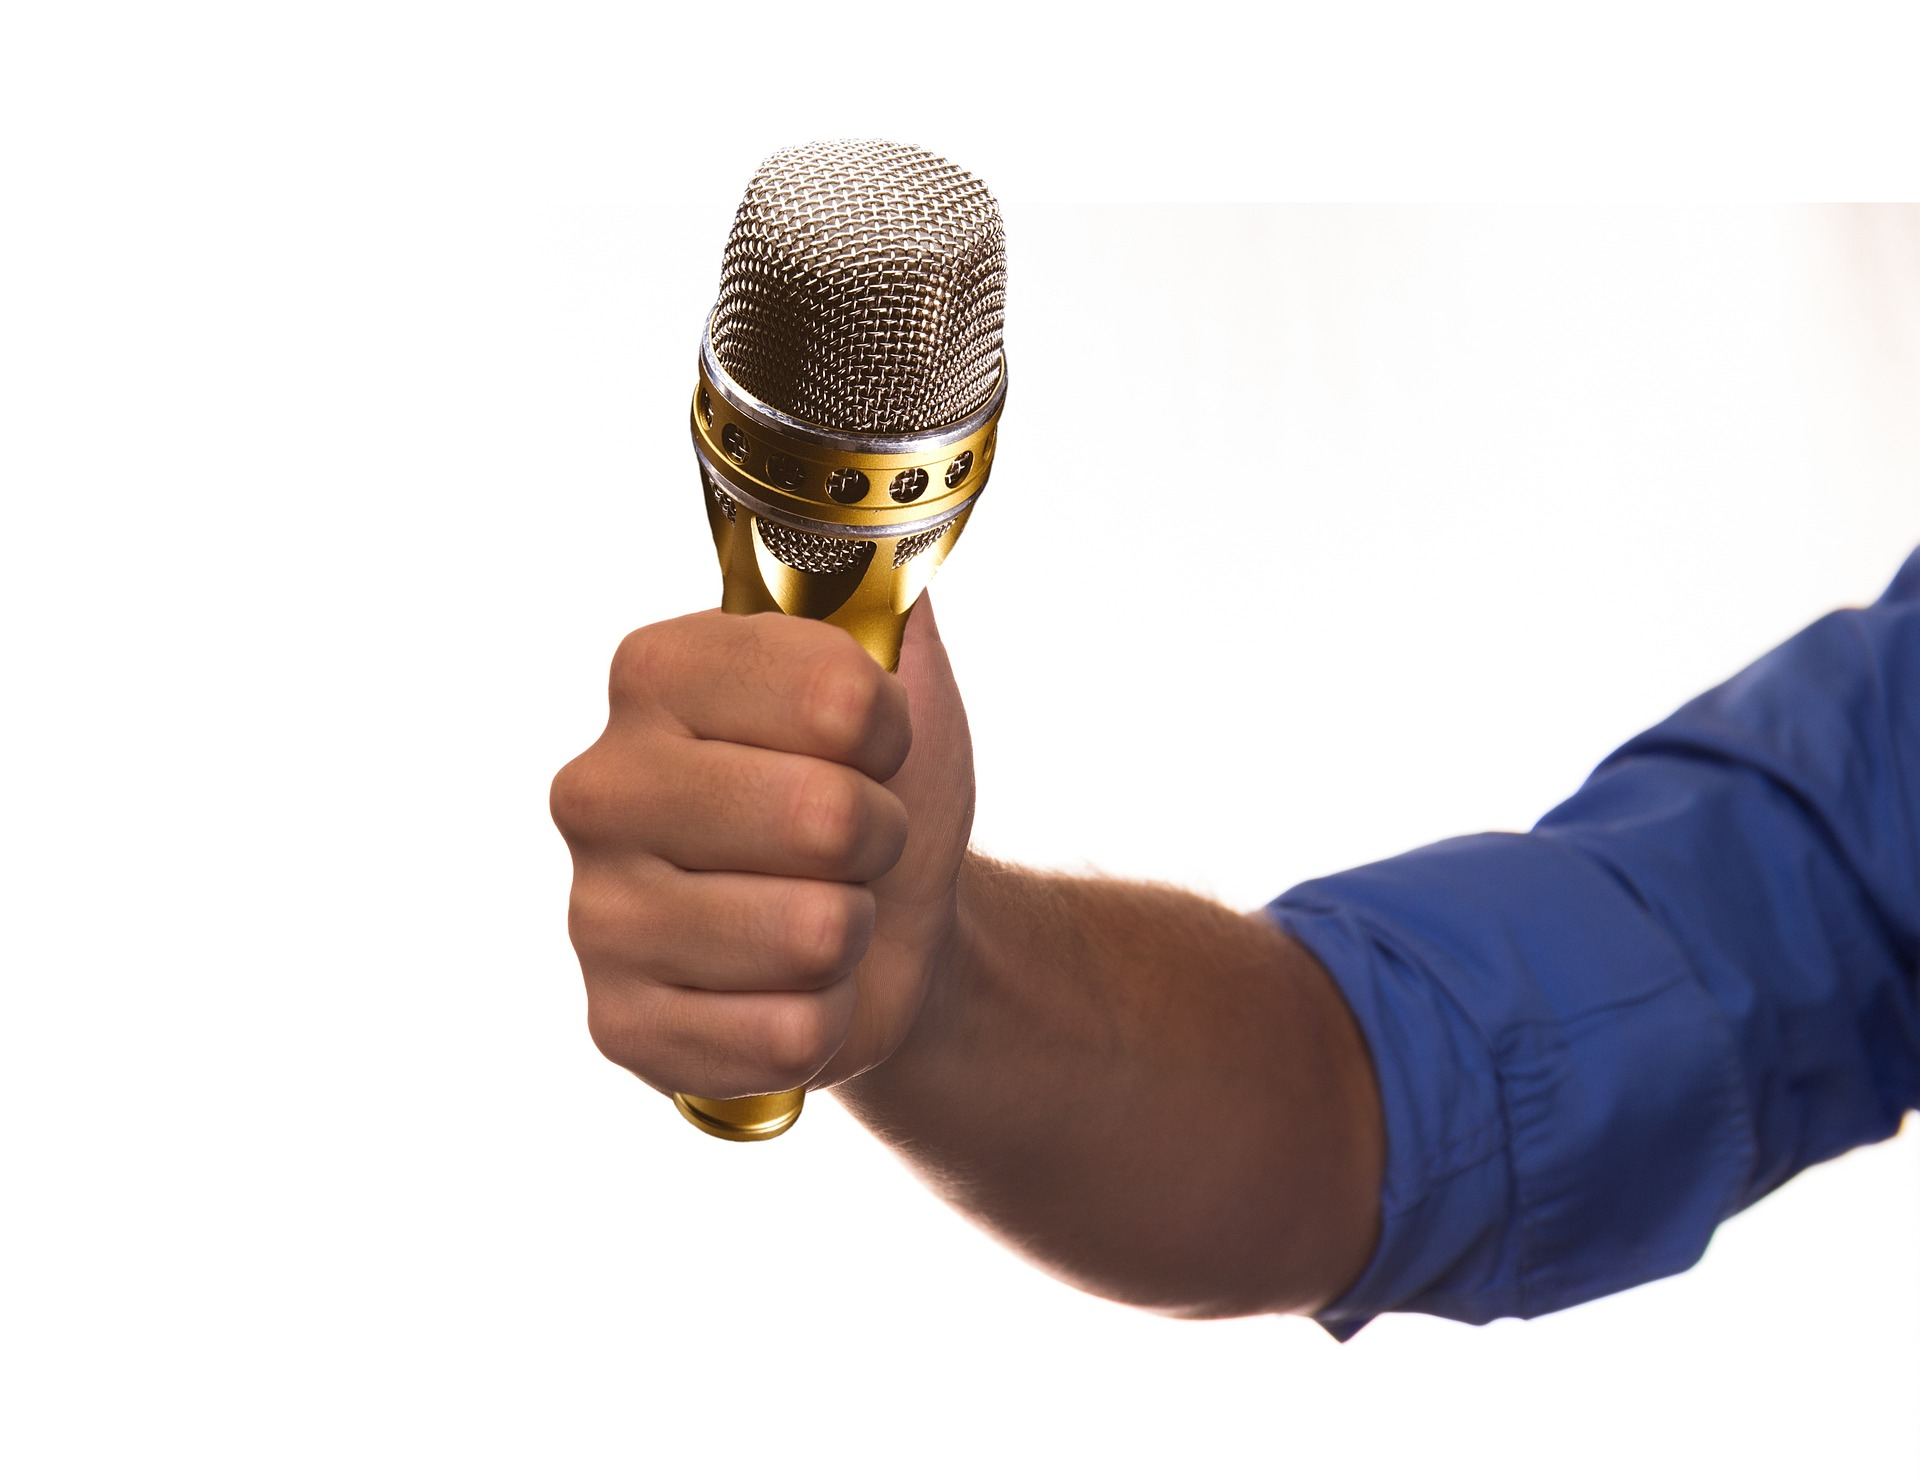
\includegraphics[width=0.25\textwidth,height=\textheight]{fig/interview.jpg}
\caption[\label{fig:interview} Interview]{\label{fig:interview} Interview\footnotemark{}}
\end{figure}
\footnotetext{The picture is free to use under the Pixabay license, see: \url{https://pixabay.com/images/id-4799256/}}

An interview is normally a one-on-one verbal conversation. Interviews are conducted to learn about the participants' experiences, perceptions, opinions, or motivations. The relationship between the interviewer and interviewee must be taken into account and other circumstances (place, time, face to face, email, etc.) should be taken into account.
There are three types of interviews structured, semi-structured, and unstructured.
\emph{Structured interviews} use a set list of questions and hence are like a verbal surveys. In \emph{unstructured interviews} the interviewer doesn't use predetermined questions but only a list of topics to address. Semi-structured interviews are the middle ground. Semi-structured interviews require the interviewer to have a list of questions and topics pre-prepared, which can be asked in different ways with different interviewee/s. Semi-structured interviews increase the flexibility and the responsiveness of the interview while keeping the interview on track, increasing the reliability and credibility of the data. Semi-structured interviews are one of the most common interview techniques.

Structured interviews use a predetermined list of questions that must be asked in a specific order, improving the validity and trustworthiness of the data but lowering respondent response. Structured interviews resemble verbal questionnaires.
In unstructured interviews, the interviewer has a planned list of subjects to cover but no predetermined interview questions. In exchange for less reliable data, this makes the interview more adaptable. Long-term field observation studies may employ unstructured interviews.
The middle ground are interviews that are semi-structured. In semi-structured interviews, the interviewer must prepare a list of questions and themes that can be brought up in various ways with various interviewees.

Interviews allow you to address a cause-and-effect relationship fairly directly, and it can be a good idea to interview experts and ask some \emph{why} and \emph{how} questions to gather initial knowledge about a particular topic before further elaborating your research strategy. For example, I interviewed kindergarten teachers with many years of experience working with children, as well as other parents, to get information on how to solve the problem of my children throwing plates around the dining room.
However, findings based on interviews are not very valid or reliable because the personal perceptions of both the interviewer and the interviewee can have an impact on the conclusions drawn. For example, I received very different tips and explanations because of the personal experiences of the people I interviewed. Unfortunately, I could not really ask my son why he was misbehaving. His vocabulary was too limited at the time, and even if he could speak, he would probably refuse to tell me the truth.

\hypertarget{surveys}{%
\subsection{Surveys}\label{surveys}}

\begin{figure}
\centering
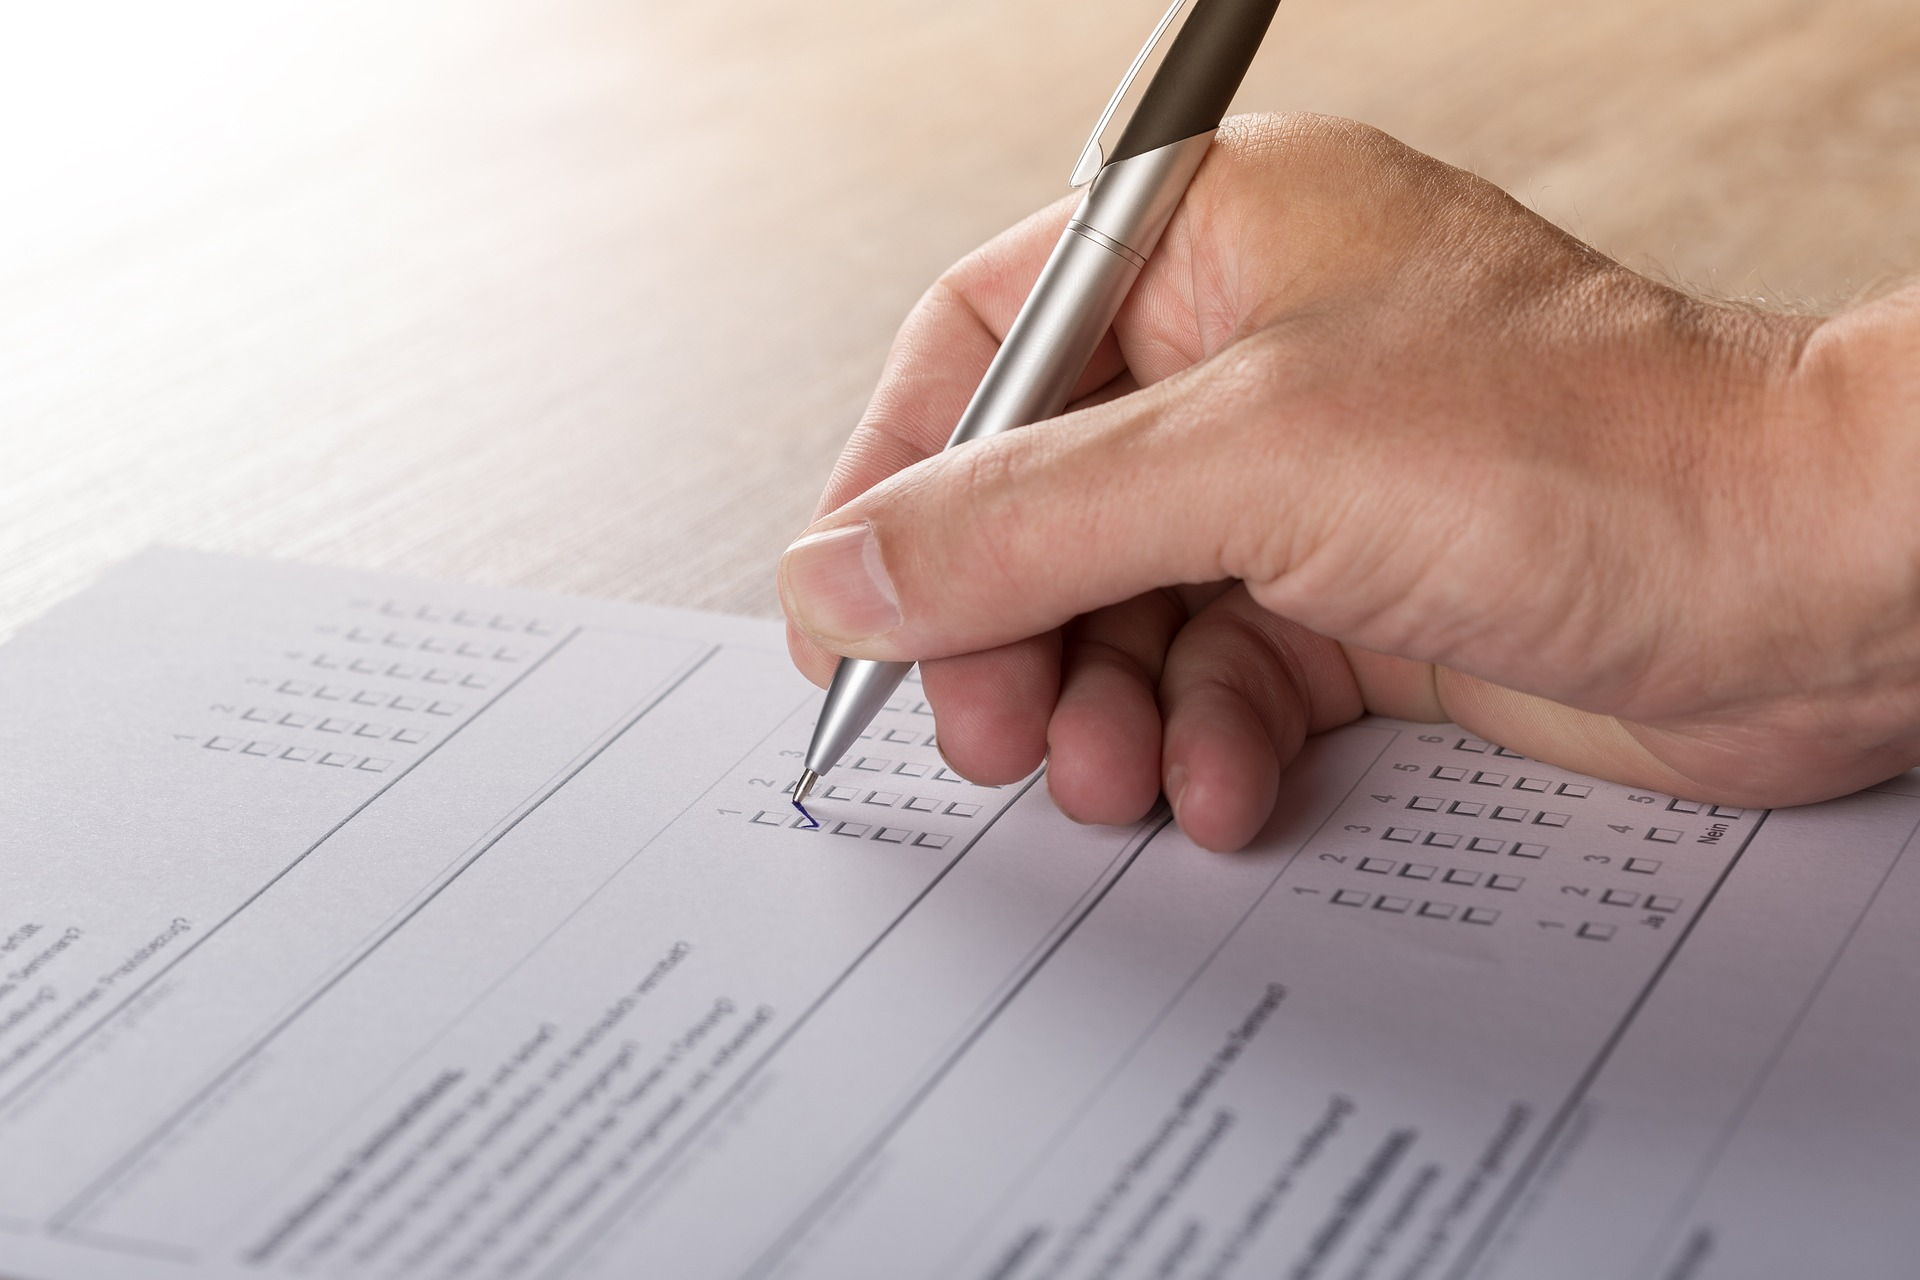
\includegraphics[width=0.25\textwidth,height=\textheight]{fig/opinion-poll.jpg}
\caption[\label{fig:survey} Survey]{\label{fig:survey} Survey\footnotemark{}}
\end{figure}
\footnotetext{The picture is free to use under the Pixabay license, see: \url{https://pixabay.com/images/id-1594962/}}

In contrast to an interview a survey can be sent out to many different people. Surveys can be used to identify a cause-and-effect relationship by asking questions about both the cause and the effect and examining the responses. For example, if a researcher wanted to determine whether there is a relationship between a person's level of education and their income, they could conduct a survey asking participants about their education level and their income. If the data shows that participants with higher levels of education tend to have higher incomes, it suggests that education may be a cause of higher income. However, it is important to note that surveys can only establish a correlation between variables, but it is difficult to claim that correlations that where found through the survey imply a causal relationship. To establish a causal relationship, a researcher would need to use other methods, such as an experiment, to control for other potential factors that might influence the relationship that the respondent does not see.

\hypertarget{case-studies}{%
\subsection{Case studies}\label{case-studies}}

\begin{figure}
\centering
\includegraphics[width=0.25\textwidth,height=\textheight]{fig/pexels-rodnae-productions-7947753.jpg}
\caption[\label{fig:casestudy} Case study]{\label{fig:casestudy} Case study\footnotemark{}}
\end{figure}
\footnotetext{Picture is free to use and stems from RODNAE Productions and was taken from Pexels: \url{https://www.pexels.com/de-de/foto/linse-geschaft-papier-aufsicht-7947753/}}

Case studies involve in-depth examination of a single case or a small number of cases in order to understand a particular phenomenon. Case studies can be conducted using both quantitative and qualitative methods, depending on the research question and the data being analyzed. While it is reasonable to find causal effects in the particular case, it is problematic to generalize the causal relationship. To establish a general causal relationship, a researcher would need to use other methods, such as an experiment, to control for other potential factors that might influence the relationship that the respondent does not see.

\hypertarget{experiments}{%
\subsection{Experiments}\label{experiments}}

One way to clearly identify a cause-and-effect relationship is through experiments, which involve manipulating the cause (the independent variable) and measuring the effect (the dependent variable) under controlled conditions (we will later on define precisely what is meant here). Experiments can be conducted using both quantitative and qualitative methods. Here are some examples:

\begin{itemize}
\tightlist
\item
  A medical study in which a new drug is tested on a group of patients, while a control group receives a placebo.
\item
  An educational study in which a group of students is taught a new method of learning, while a control group is taught using the traditional method.
\item
  An agricultural study in which a group of crops is treated with a new fertilization method, while a control group is not treated.
\item
  A study to determine the effect of a new training program on employee productivity might involve randomly assigning employees to either a control group that does not receive the training, or an experimental group that does receive the training. By comparing the productivity of the two groups, the researchers can determine if the new training program had a causal effect on employee productivity.
\item
  A study to determine the effect of a new advertising campaign on sales might involve randomly assigning different groups of customers to be exposed to different versions of the campaign. By comparing the sales of the different groups, the researchers can determine if the advertising campaign had a causal effect on sales.
\item
  In \emph{experimental economics}, experimental methods are used to study economic questions. In a lab-like environment data are collected to investigate the size of certain effects, to test the validity of economic theories, to illuminate market mechanisms, or to examine the decision making of people. Economic experiments usually motivates and rewards subjects with money. The overall goal is to mimic real-world incentives and investigate things that cannot be captured or identified in the field.
\item
  In \emph{behavioral economics}, laboratory experiments are also used to study decisions of individuals or institutions and to test economic theory. However, it is done with a focus on cognitive, psychological, emotional, cultural, and social factors.
\end{itemize}

\begin{figure}
\centering
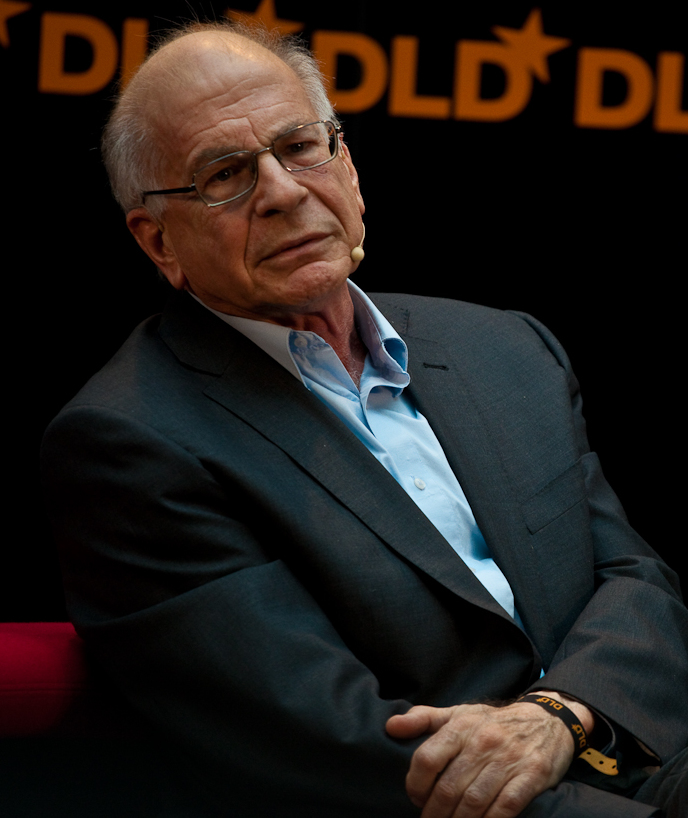
\includegraphics[width=0.3\textwidth,height=\textheight]{fig/Daniel_Kahneman.jpg}
\caption[\label{fig:dkahnemann} Daniel Kahneman (*1934)]{\label{fig:dkahnemann} Daniel Kahneman (*1934)\footnotemark{}}
\end{figure}
\footnotetext{The picture of Kahneman is free to use and stems from \url{https://commons.wikimedia.org/wiki/File:Daniel_Kahneman_(3283955327)_(cropped).jpg}}

\begin{figure}
\centering
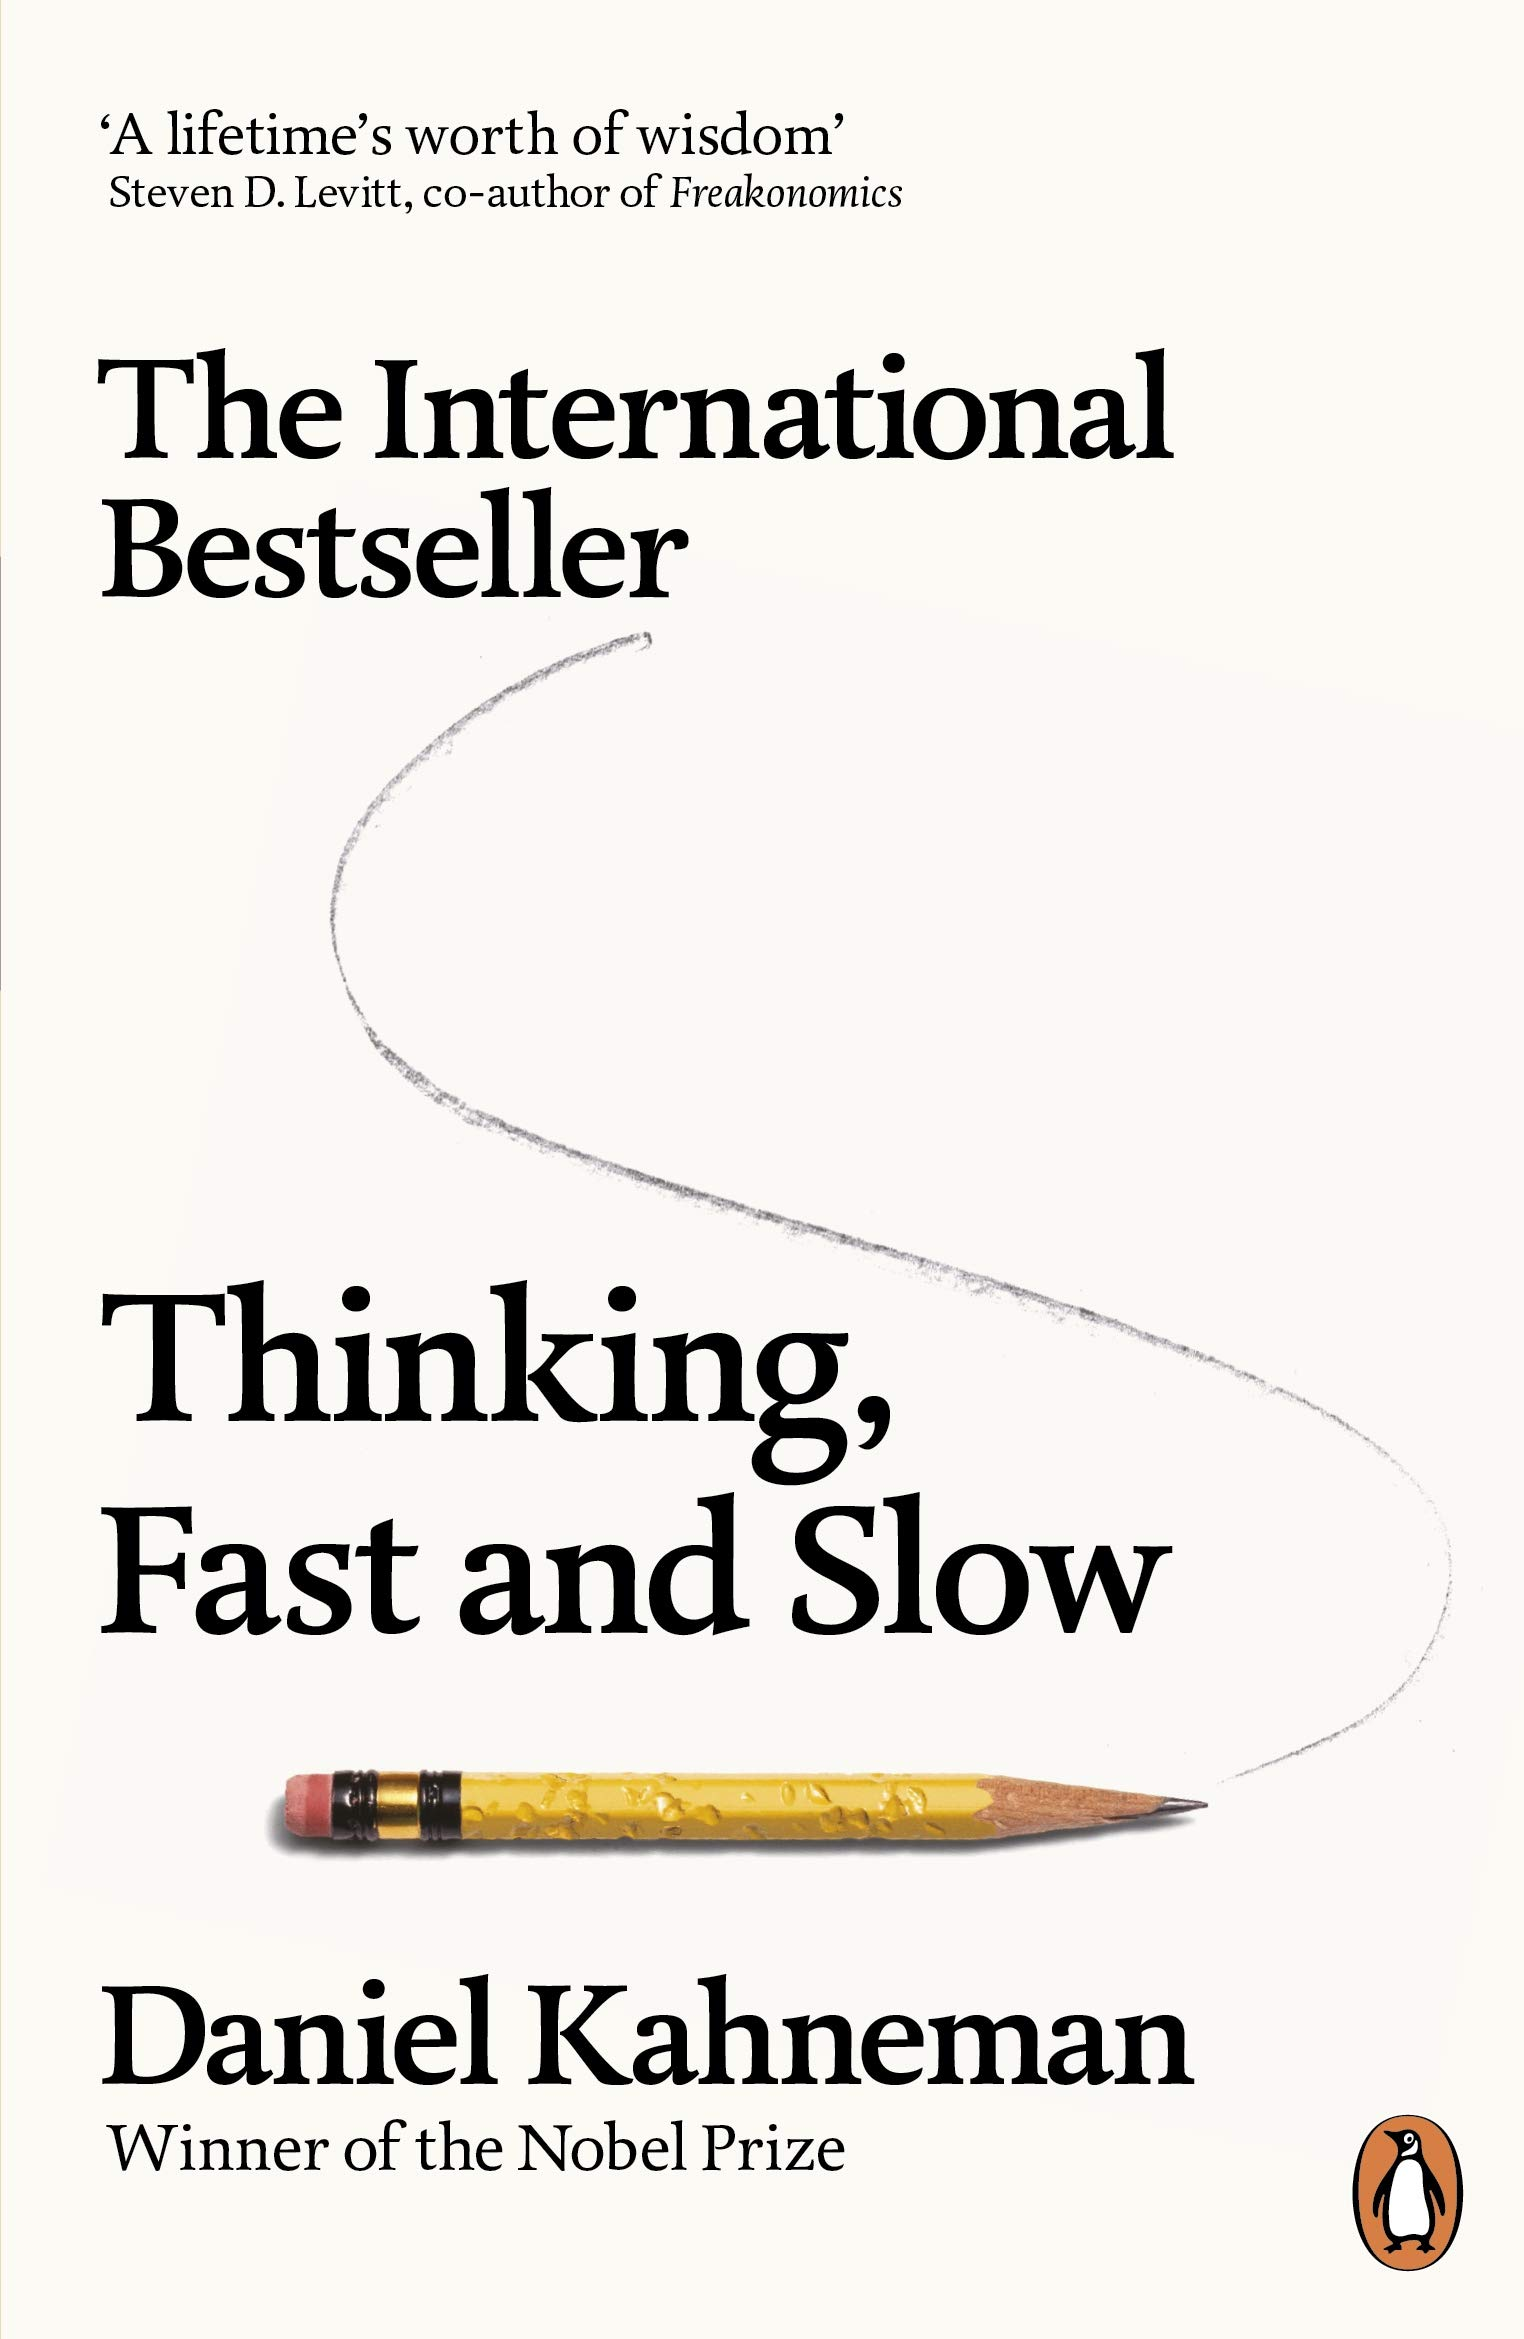
\includegraphics[width=0.25\textwidth,height=\textheight]{fig/tfts.jpg}
\caption{\label{fig:dkahnemann2} \citet{Kahneman2011Thinking}: Thinking, Fast and Slow}
\end{figure}

In 2002 the Nobel Prize of Economics was awarded to Vernon L. Smith ``for having established \emph{laboratory experiments} as a tool in empirical economic analysis, especially in the study of alternative market mechanisms'' \citep{RSAS2002} and Daniel Kahneman ``for having integrated insights from psychological research into economic science, especially concerning human judgment and decision-making under uncertainty'' \citep{RSAS2002}.

The strength of evidence from a controlled experiment is generally considered to be strong. However, the external validity, i.e., the generalizability, should be considered as well. External validity is sometimes low because effects that you can identify and measure in a lab are sometimes only of minor importance in the field.

There are different types of experiments:

\textbf{Randomized controlled trials (RCTs)} are a specific type of an experiment that involve randomly assigning participants to different treatment groups and comparing the outcomes of those groups. RCTs are often considered the gold standard of experimental research because they provide a high degree of control over extraneous variables and are less prone to bias.

For a better explanation and some great insights into what an RCT actually is, please watch the video produced by UNICEFInnocenti and published on the YouTube channel of UNICEF's dedicated research center \url{https://youtu.be/Wy7qpJeozec}

\begin{figure}
\centering
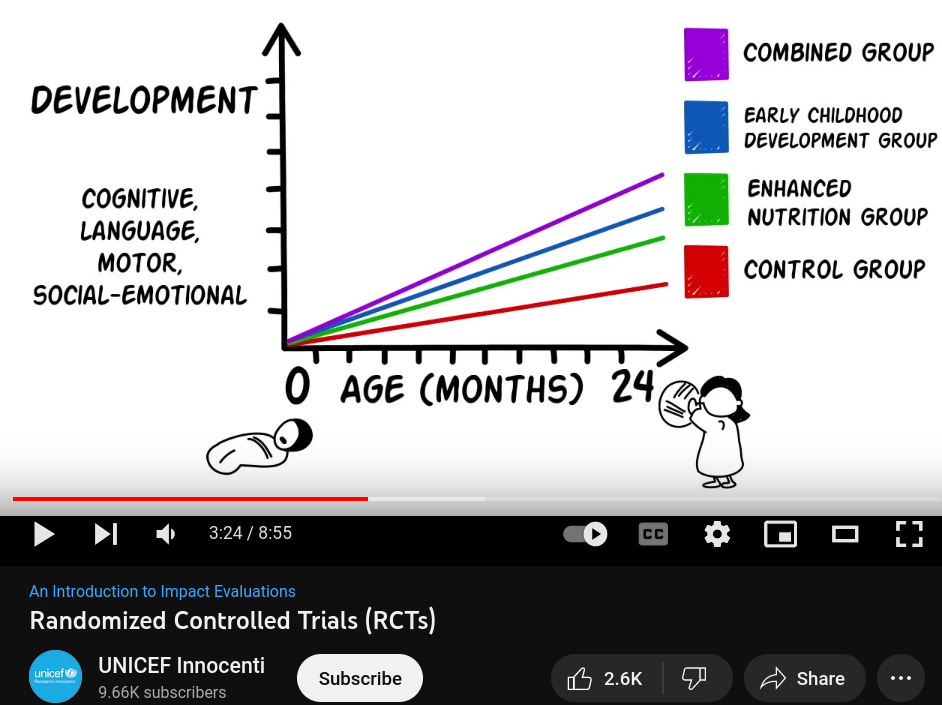
\includegraphics[width=0.5\textwidth,height=\textheight]{fig/rcts-video.png}
\caption{\label{fig:rcts} Randomized Controlled Trials (RCTs)}
\end{figure}

\textbf{Quasi-experiments} involve the manipulation of an independent variable, but do not involve random assignment of participants to treatment groups. Quasi-experiments are less controlled than RCTs, but can still provide valuable insights into cause-and-effect relationships.

\textbf{Natural experiments} involve the observation of naturally occurring events or situations that provide an opportunity to study cause-and-effect relationships. Natural experiments are often used when it is not possible or ethical to manipulate variables experimentally.

In a \textbf{laboratory experiment}, researchers manipulate an independent variable and measure the effect on a dependent variable in a controlled laboratory setting. This allows for greater control over extraneous variables, but the results may not generalize to real-world situations.

In a \textbf{field experiment}, researchers manipulate an independent variable and measure the effect on a dependent variable in a natural setting, rather than in a laboratory. This allows researchers to study real-world phenomena, but it can be more difficult to control for extraneous variables.

\hypertarget{observational-data}{%
\subsection{Observational data}\label{observational-data}}

\begin{figure}
\centering
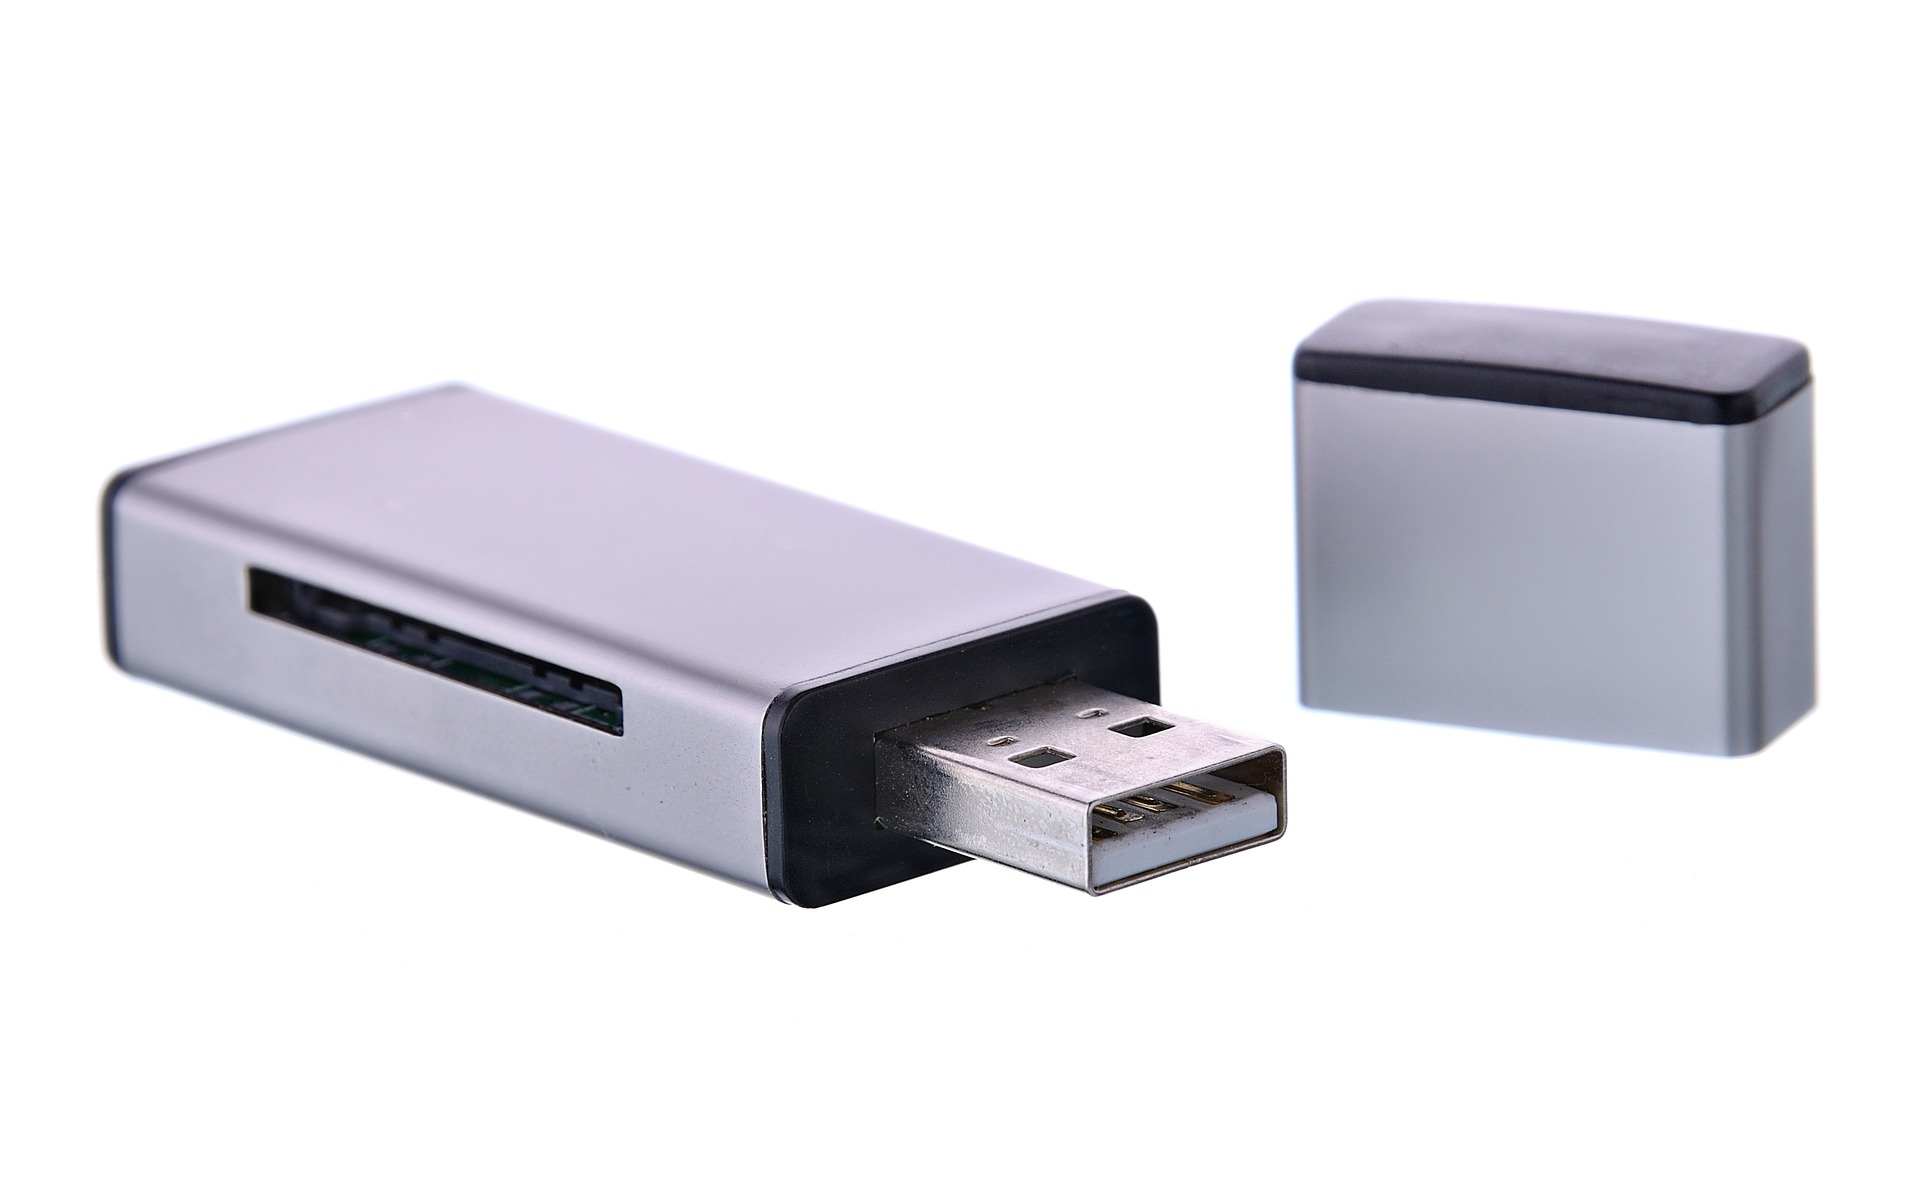
\includegraphics[width=0.25\textwidth,height=\textheight]{fig/usb.jpg}
\caption[\label{fig:observationaldata} Observational data]{\label{fig:observationaldata} Observational data\footnotemark{}}
\end{figure}
\footnotetext{The picture is free to use under the Pixabay license, see: \url{https://pixabay.com/images/id-5029286/}}

Observational data are data that had been observed before the research question was asked or being collected independently from the study.
To understand how observational data can be used to constitute a causal relationship is a bit tricky because there is only one world and only one reality at a time. In other words, we usually miss a counterfactual which we can use for a comparison. Take, for example, the past COVID-19 pandemic, where you chose to be vaccinated or not. Regardless of what you chose, we will never find out what would have happened to you if you had chosen differently. Maybe you would have died, maybe you would have gotten more or less sick, or maybe you wouldn't have gotten sick at all. We don't know, and it's impossible to find out because it's impossible to observe the counterfactual outcomes. This makes it difficult to establish causality from observational data. However, ingenious minds have found reasonable procedures and methods to extract some level of knowledge from observational data that allows us to infer causal relationships from observational data where we cannot directly observe the counterfactual outcome. We will come back to these methods later on.

In the upcoming sections, however, we will discuss experimental research designs including \emph{randomized controlled trials} (RCTs) which are considered to be the ``gold standard for measuring the effect of an action'' \citep[p.~128]{Taddy2019Business}. RCTs can be used, for example, to study the effectiveness of drugs by observing people randomly assigned to three groups, one taking the pill (or treatment), a second receiving a placebo, and a third taking nothing. If the first group responds in any way differently than the other groups, the drug has an effect. Before explaining an RCT in more detail, we need to be clear about the fundamental problem of causal inference. This will be discussed in the following.

\begin{exercise}
\protect\hypertarget{exr:methodsinresearch}{}\label{exr:methodsinresearch}Methods used in economic research

Read \citet{Paldam2021Methods} which is freely available, see \url{https://doi.org/10.1515/econ-2021-0003} and answer the following questions:

\begin{enumerate}
\def\labelenumi{\alph{enumi})}
\tightlist
\item
  List the eight types of research methods described in the paper and provide the description found in the paper.
\item
  Read the following statements and discuss whether they are true or not, and if the latter, correct them:

  \begin{enumerate}
  \def\labelenumii{\roman{enumii})}
  \tightlist
  \item
    The annual production of research papers in economics in the year 2017 has reached about 100 papers in top journals, and about 1,400 papers in the group of good journals. The production has grown with 3.3\% per year, and thus it has doubled the last twenty years.
  \item
    The upward trend in publication must be due to the large increase in the importance of publications for the careers of researchers, which has greatly increased the production of papers. There has also been a large increase in the number of researches, but as citations are increasingly skewed toward the top journals it has not increased demand for papers correspondingly.
  \item
    Four trends are significant: The fall in theoretical papers and the rise in classical papers. There is also a rise in the share of statistical method and event studies. It is surprising that there is no trend in the number of experimental studies.
  \item
    Book reviews have dropped to less than 1/3. Perhaps, it also indicates that economists read fewer books than they used to. Journals have increasingly come to use smaller fonts and larger pages, allowing more words per page. The journals from North-Holland Elsevier have managed to cram almost two old pages into one new one. This makes it easier to publish papers, while they become harder to read.
  \item
    About 50\% of papers in the sample considered in \cite{Paldam2021Methods} belong to the economic theory class, about 6\% are experimental studies, and about 43\% are empirical studies based on data inference.
  \item
    The papers in economic theory have increased from 33.6\% to 59.5\% -- this is the largest change for any of the eight subgroups. It is highly significant in the trend test.
  \end{enumerate}
\item
  Explain what is meant with \textit{theory fatigue} and discuss the reasons that lead to that fatigue.
\item
  What makes according to \cite{Paldam2021Methods} research papers relevant for policymakers right from the start?
\end{enumerate}

Please find solution to the exercise \protect\hyperlink{sol:methodsinresearch}{here}.
\end{exercise}

\hypertarget{sol:methodsinresearch}{%
\subsection*{Solution to exercise \ref{exr:methodsinresearch}: Methods used in economic research}\label{sol:methodsinresearch}}

\begin{enumerate}
\def\labelenumi{\alph{enumi})}
\tightlist
\item
\end{enumerate}

\begin{enumerate}
\def\labelenumi{\arabic{enumi}.}
\item
  \textbf{Economic theory:} Papers are where the main content is the development of a theoretical model. The ideal theory paper presents a (simple) new model that recasts the way we look at something important.
\item
  \textbf{Statistical technique, incl.~forecasting} Papers reporting new estimators and tests are published in a handful of specialized journals in econometrics and mathematical statistics. Some papers compare estimators on actual data sets. If the demonstration of a methodological improvement is the main feature of the paper, it belongs to this subgroup, but if the economic interpretation is the main point of the paper, it belongs to the classical empirical studies or newer techniques group.
\item
  \textbf{Surveys, incl.~meta-studies} When the literature in a certain field becomes substantial, it normally presents a motley picture with an amazing variation, especially when different schools exist in the field. They are of two types, where the second type is still rare:
\end{enumerate}

\begin{itemize}
\tightlist
\item
  Firstly, assessed surveys where the author reads the papers and assesses what the most reliable results are. Such assessments require judgment that is often quite difficult to distinguish from priors, even for the author of the survey.
\item
  Secondly, meta-studies which are quantitative surveys of estimates of parameters claimed to be the same. These types of studies have two levels: The basic level collects and codes the estimates and studies their distribution. This is a rather objective exercise where results seem to replicate rather well. The second level analyzes the variation between the results. This is less objective.
\end{itemize}

\begin{enumerate}
\def\labelenumi{\arabic{enumi}.}
\setcounter{enumi}{3}
\item
  \textbf{Experiments in laboratories} Most of these experiments take place in a laboratory, where the subjects communicate with a computer, giving a controlled, but artificial, environment. A number of subjects are told a (more or less abstract) story and paid to react in either of a number of possible ways. A great deal of ingenuity has gone into the construction of such experiments and in the methods used to analyze the results. Lab experiments do allow studies of behavior that are hard to analyze in any other way, and they frequently show sides of human behavior that are difficult to rationalize by economic theory. However, everything is artificial -- even the payment while participants usually receive real money for participation and their performance. In some cases, the stories told are so elaborate and abstract that framing must be a substantial risk. In addition, experiments cost money, which limits the number of subjects. It is also worth pointing to the difference between expressive and real behavior. It is typically much cheaper for the subject to `express' nice behavior in a lab than to be nice in the real world.
\item
  \textbf{Event studies (field experiments and natural experiments)} Event studies are studies of real world experiments. They are of two types:
\end{enumerate}

\begin{itemize}
\tightlist
\item
  Firstly, \textbf{field experiments} analyze cases where some people get a certain treatment and others do not. The `gold standard' for such experiments is double blind random sampling, where everything (but the result!) is announced in advance. Experiments with humans require permission from the relevant authorities, and the experiment takes time too. In the process, things may happen that compromise the strict rules of the standard. Controlled experiments are expensive, as they require a team of researchers.
\item
  Secondly, \textbf{natural experiments} take advantage of a discontinuity in the environment, i.e., the period before and after an (unpredicted) change of a law, an earth-quake, etc. Methods have been developed to find the effect of the discontinuity. Often, such studies look like classical empirical studies with many controls that may that may or may not belong. Thus, the problems discussed under the classic empirical studies also apply here.
\end{itemize}

\begin{enumerate}
\def\labelenumi{\arabic{enumi}.}
\setcounter{enumi}{5}
\item
  \textbf{Descriptive, deductions from data} In a descriptive study, researcher use an existing sample and hence, they have no control over the data generating process as it is usually the case with experiments. Descriptive studies are deductive. The researcher describes the data aiming at finding structures that tell a story, which can be interpreted. The findings may call for a formal test. If one clean test follows from the description, the paper can still be classified as a descriptive study. If more elaborate regression analysis is used, however, it can also be classified as a classical empirical study. Descriptive studies often contain a great deal of theory. Some descriptive studies present a new data set developed by the author to analyze a debated issue. In these cases, it is often possible to make a clean test, so to the extent that biases sneak in, they are hidden in the details of the assessments made when the data are compiled.
\item
  \textbf{Classical empirical studies}
  Typically have three steps: It starts by a theory, which is developed into an operational model. Then it presents the data set, and finally it runs regressions. The significance levels of the t-ratios on the coefficient estimated assume that the regression is the first meeting of the estimation model and the data. In practice, we all know that this is rarely the case. The classical method is often just a presentation technique. The great virtue of the method is that it can be applied to real problems outside academia. The relevance comes with a price: The method is quite flexible as many choices have to be made, and they often give different results. Preferences and interests, may affect these choices.
\item
  \textbf{Newer techniques}
  Partly as a reaction to the problems of classical empirical methods, the last 3--4 decades have seen a whole set of newer empirical techniques. They include different types of vector autoregression (VAR)\footnote{A VAR is a statistical model used to capture the relationship between multiple quantities as they change over time.}, Bayesian techniques, causality and co-integration tests, Kalman filters, hazard functions, etc. The main reason for the lack of success for the new empirics is that it is quite bulky to report a careful set of co-integration tests or VARs, for example, and they often show results that are far from useful in the sense that they are unclear and difficult to interpret.
\end{enumerate}

\begin{enumerate}
\def\labelenumi{\alph{enumi})}
\setcounter{enumi}{1}
\tightlist
\item
  Solutions to b)
\end{enumerate}

\begin{itemize}
\item
  \begin{enumerate}
  \def\labelenumi{\roman{enumi})}
  \tightlist
  \item
    The annual production of research papers in economics in the year 2017 has now reached about \textbf{1,000} papers in top journals, and about \textbf{14,000} papers in the group of good journals. The production has grown with 3.3\% per year, and thus it has doubled the last twenty years.
  \end{enumerate}
\item
  \begin{enumerate}
  \def\labelenumi{\roman{enumi})}
  \setcounter{enumi}{1}
  \tightlist
  \item
    Statement is correct.
  \end{enumerate}
\item
  \begin{enumerate}
  \def\labelenumi{\roman{enumi})}
  \setcounter{enumi}{2}
  \tightlist
  \item
    Statement is correct.
  \end{enumerate}
\item
  \begin{enumerate}
  \def\labelenumi{\roman{enumi})}
  \setcounter{enumi}{3}
  \tightlist
  \item
    Statement is correct.
  \end{enumerate}
\item
  \begin{enumerate}
  \def\labelenumi{\alph{enumi})}
  \setcounter{enumi}{21}
  \tightlist
  \item
    Statement is correct.
  \end{enumerate}
\item
  \begin{enumerate}
  \def\labelenumi{\roman{enumi})}
  \setcounter{enumi}{5}
  \tightlist
  \item
    The papers in economic theory have \textbf{dropped from 59.5\% to 33.6\%} -- this is the largest change for any of the eight subgroups. It is highly significant in the trend test.
  \end{enumerate}
\end{itemize}

\begin{enumerate}
\def\labelenumi{\alph{enumi})}
\setcounter{enumi}{2}
\item
  Theory fatigue simply explains the declining attractiveness of theoretical research for journals, researchers, and policymakers that can be justified or accompanied by an increasing importance of empirical research. Variations of existing theoretical models are more difficult to sell to policymakers and it is hard for researchers to summarize the knowledge of theoretical papers in a systematic way and to conclude on a certain topic. Moreover, theoretical papers can be very unconvincing and can hardly be understood by a broader audience which has to grant that the calculations are done right. Often, believability hinges on the realism of the assumptions at the start and of the results presented at the end. In order for a model to convince, it should (at least) demonstrate the realism of either the assumptions or the outcome. If both ends appear to hang in the air, it becomes a game giving little new knowledge about the world. The theory fatigue has caused a demand for simulations demonstrating that the models can mimic something in the world. Calibrations may be carefully done, but it often appears like a numerical solution of a model that is too complex to allow an analytical solution. Thus, these calibrations cannot really solve the fatigue.
\item
  The typical classical paper provides estimates of a key effect that decision-makers outside
  academia want to know. This makes the paper policy relevant right from the start, and in
  many cases, it is possible to write a one page executive summary to the said decision-makers.
\end{enumerate}

\hypertarget{cornotcaus}{%
\section{Correlation does not imply causation}\label{cornotcaus}}

Correlation refers to a statistical relationship between two variables, where one variable tends to increase or decrease as the other variable also increases or decreases. However, just because two variables are correlated does not necessarily mean that one variable causes the other. This is known as the \emph{correlation does not imply causation} principle.

For example, it may be observed that the number of storks in a particular area is correlated with the birth rate of babies in that area. However, this does not mean that the presence of storks causes an increase in the birth rate. It is possible that both the number of storks and the number of babies born are influenced by other factors, such as the overall population density or economic conditions in the area.

Therefore, it is important to carefully consider all possible explanations (confounders) for a correlation and to use empirical evidence to determine the true cause-and-effect relationship between variables.

\begin{figure}
\centering
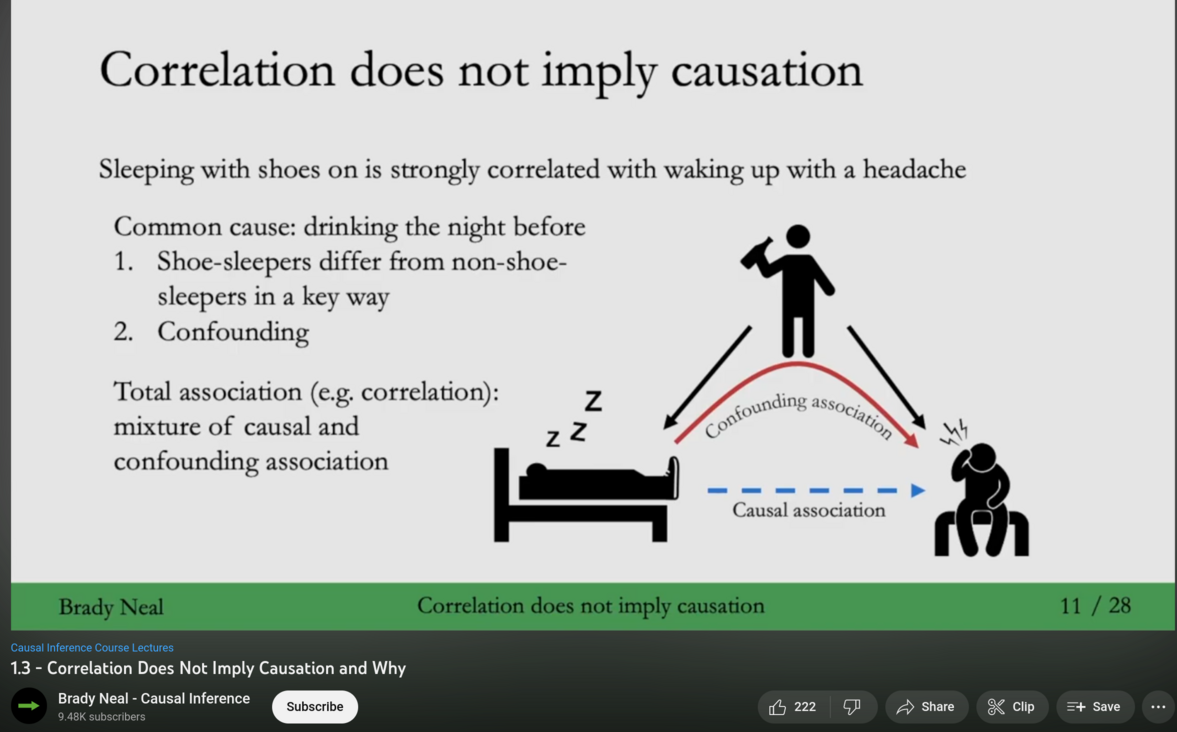
\includegraphics[width=0.5\textwidth,height=\textheight]{fig/neal1-3.png}
\caption[\label{fig:cdnic} Correlation does not imply causation]{\label{fig:cdnic} Correlation does not imply causation\footnotemark{}}
\end{figure}
\footnotetext{Picture is taken from \url{https://youtu.be/DFPm_a-_uJM}}

Watch the video of Brady Neal's lecture \href{https://youtu.be/DFPm_a-_uJM}{\emph{Correlation Does Not Imply Causation and Why}}. Alternatively, you can read chapter 1.3 of his lecture notes \citep{Neal2020Introduction} which you find \href{https://www.bradyneal.com/Introduction_to_Causal_Inference-Dec17_2020-Neal.pdf}{here}.

\hypertarget{the-fundamental-problem-of-causal-inference}{%
\section{The fundamental problem of causal inference}\label{the-fundamental-problem-of-causal-inference}}

\begin{figure}
\centering
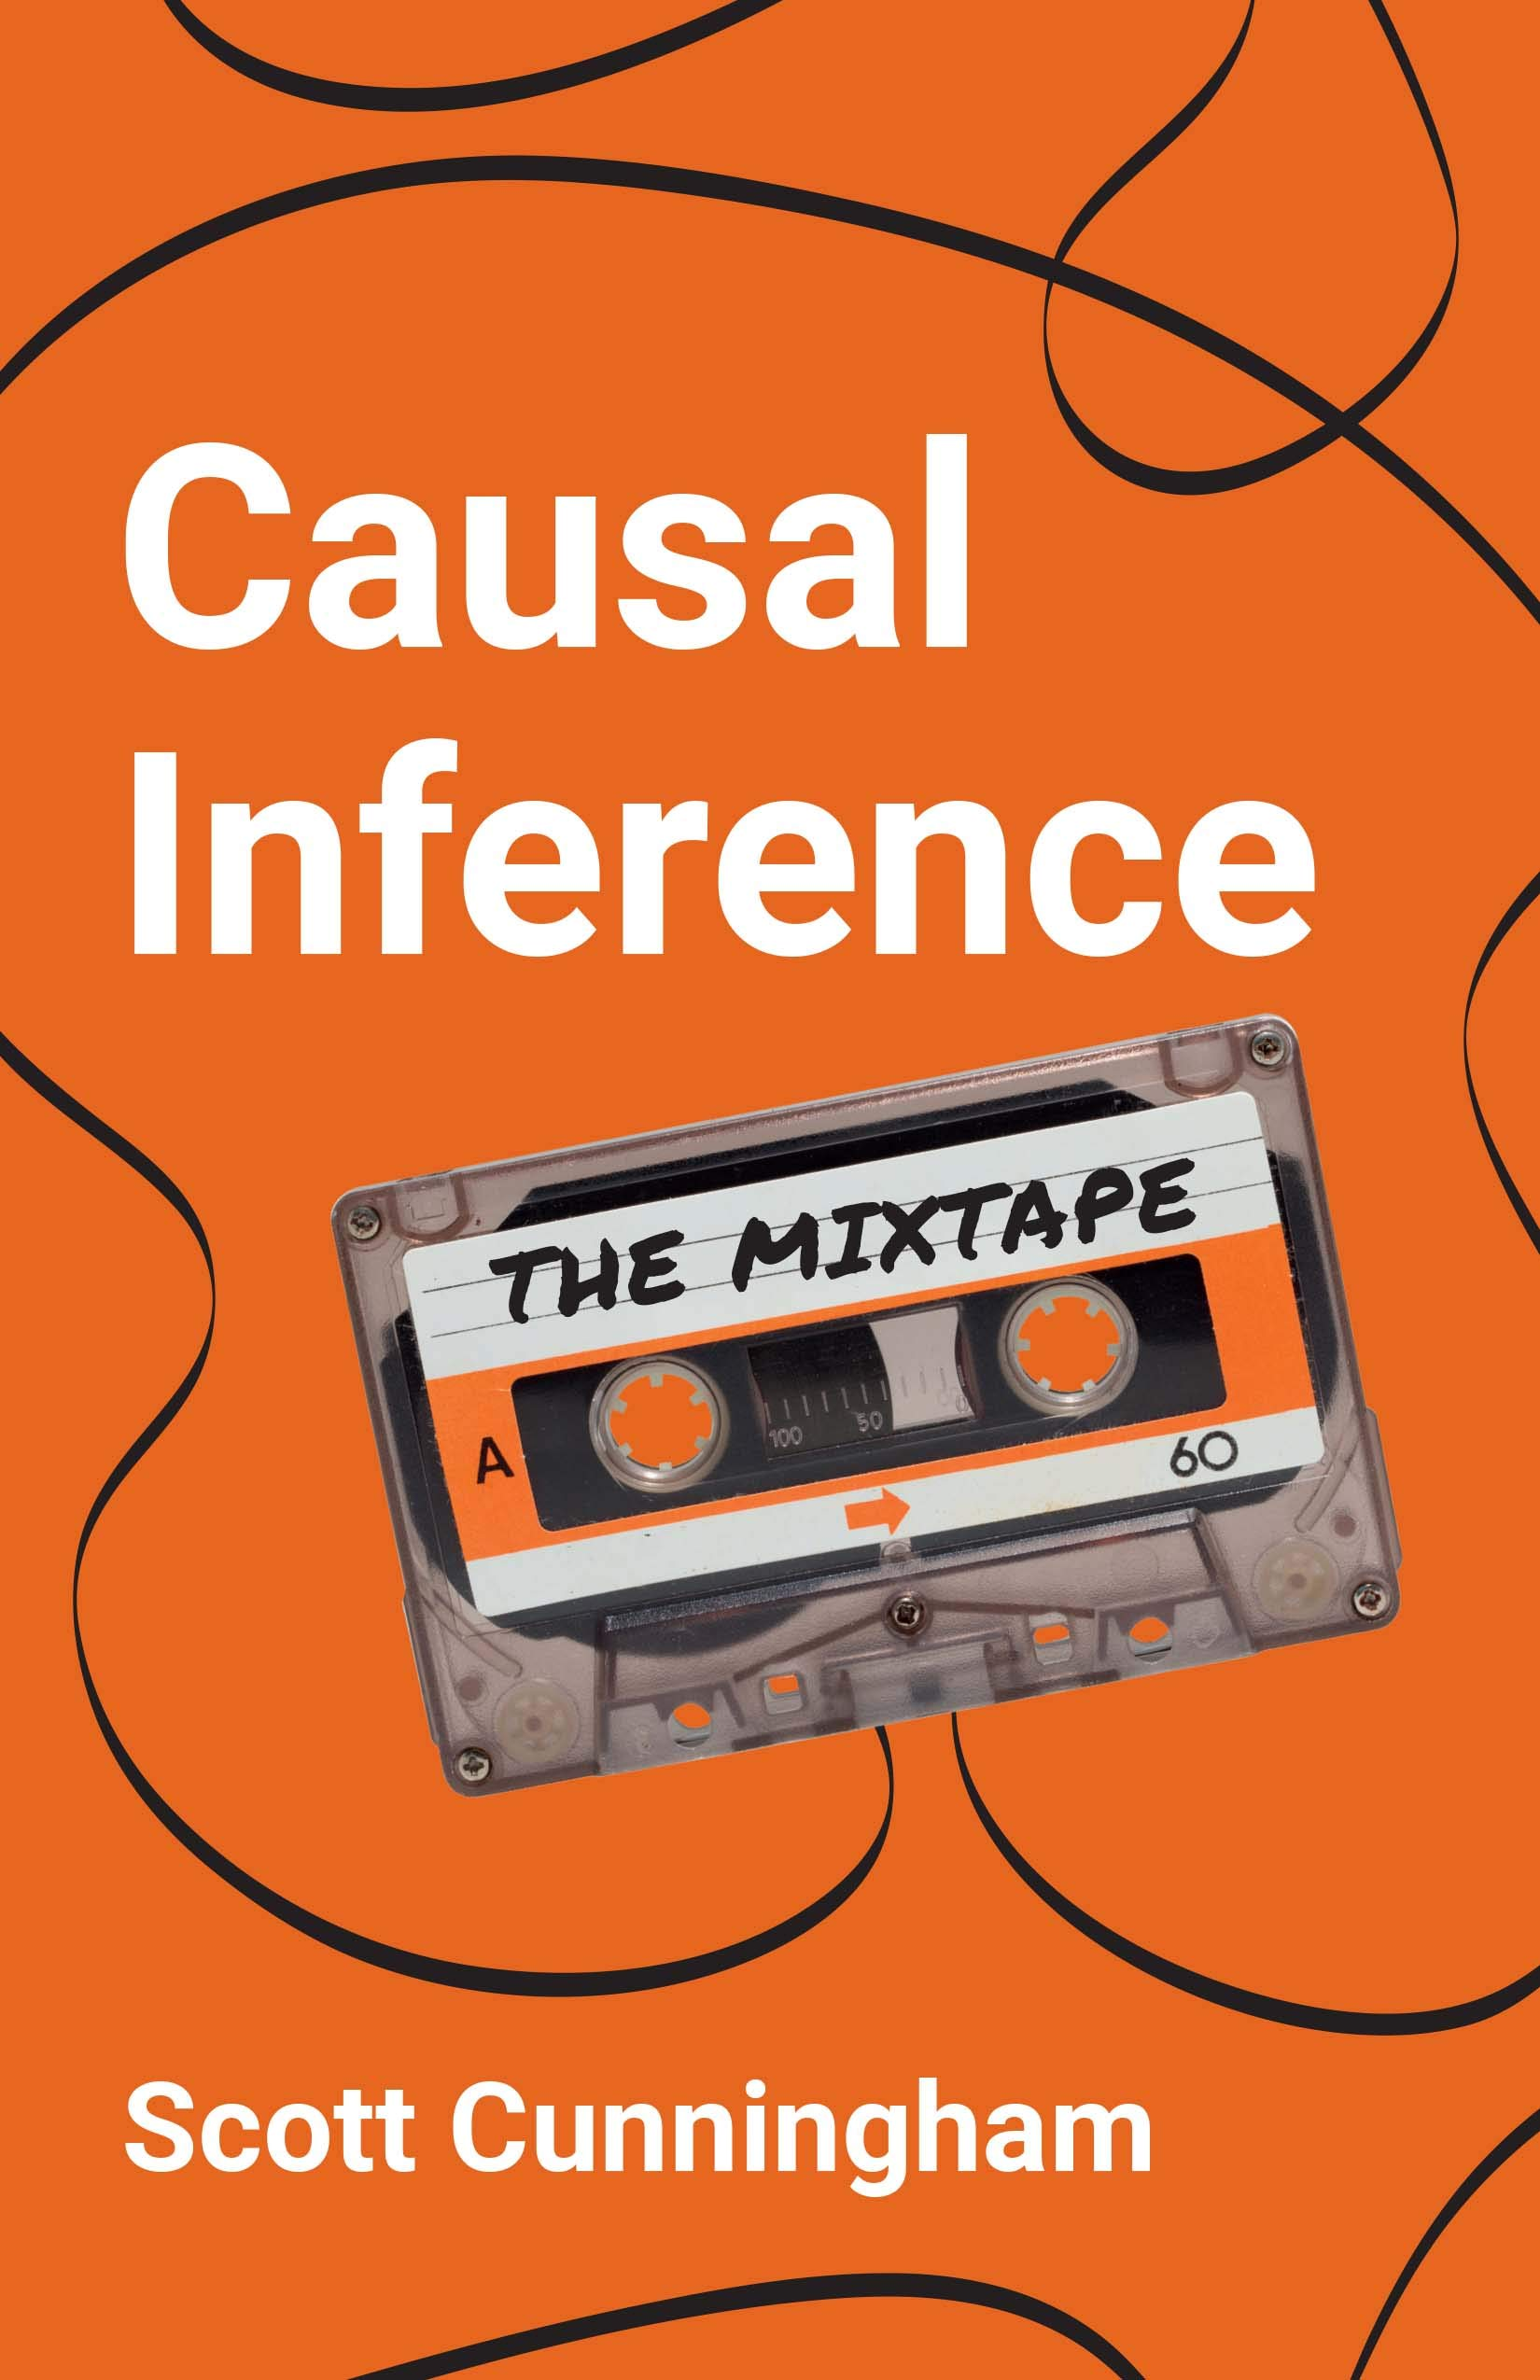
\includegraphics[width=0.1\textwidth,height=\textheight]{fig/cover-ci.jpg}
\caption{\label{fig:cunbook} The book cover of ``Causal Inference: The Mixtape?'' by Scott \citet{Cunningham2021Causal}}
\end{figure}

\begin{quote}
\citet[ch.~1.3]{Cunningham2021Causal}: \emph{``It is my firm belief, which I will emphasize over and over in this book, that without prior knowledge, estimated causal effects are rarely, if ever, believable. Prior knowledge is required in order to justify any claim of a causal finding. And economic theory also highlights why causal inference is necessarily a thorny task.''}
\end{quote}

As \citet{Cunningham2021Causal} explains in his book, it is very hard to claim causality. In the following section, I will paraphrase briefly two aspects why it is so difficult to claim to have found a causal effect. It is difficult to know how to use data properly and how to find or generate the right data. Therefore, I will discuss Simpson's Paradox and the that gives an idea how difficult it is to analyze observational data meaningful and that we need to have a theory when looking on data and we should try to challenge the assumptions on which out theory is build on. After that I will briefly discuss

\begin{exercise}
\protect\hypertarget{exr:causalinf1}{}\label{exr:causalinf1}Causal inference ch.1

Before going on with the content in these notes, please read chapter 1 (Introduction) of \citet{Cunningham2021Causal} and answer the following questions. The book is freely available (\url{https://mixtape.scunning.com/}) and the link to chapter 1 is \url{https://mixtape.scunning.com/01-introduction}.

\begin{enumerate}
\def\labelenumi{\arabic{enumi}.}
\item
  What are some common misconceptions about causality that the author addresses in chapter 1?
\item
  What is the role of randomization in causal inference, as described in the book?
\end{enumerate}

Please find solution to the exercise \protect\hyperlink{sol:causalinf1}{in the appendix.}
\end{exercise}

\hypertarget{simpsons-paradox}{%
\subsection{Simpsons Paradox}\label{simpsons-paradox}}

\begin{figure}
\centering
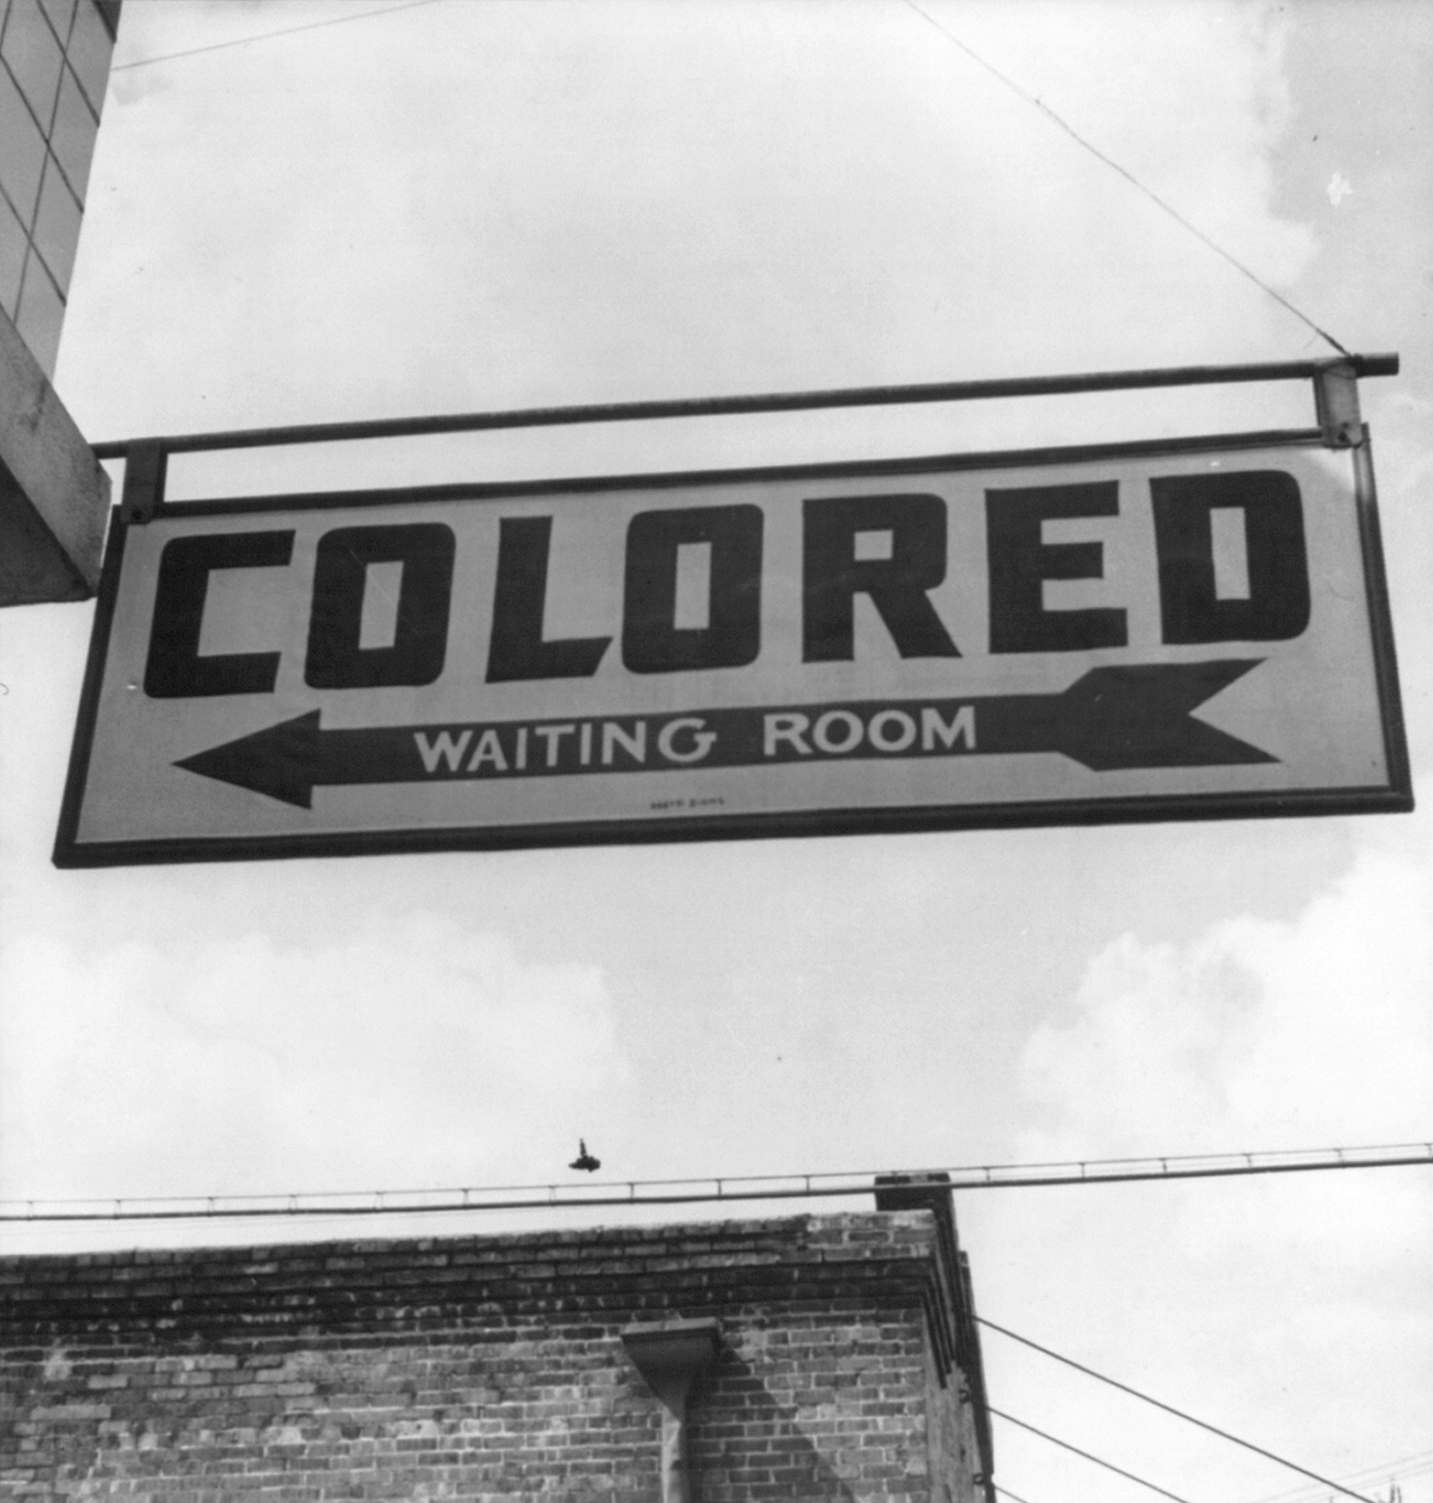
\includegraphics[width=0.25\textwidth,height=\textheight]{fig/1943_Colored_Waiting_Room_Sign.jpg}
\caption[\label{fig:waitingroom} Discrimination]{\label{fig:waitingroom} Discrimination\footnotemark{}}
\end{figure}
\footnotetext{The photography is public domain and stems from the Library of Congress Prints and Photographs Division Washington, see: \url{http://hdl.loc.gov/loc.pnp/pp.print}.}

Discrimination is bad. Whenever we see it, we should try to find ways to overcome it. De jure segregation mandated the separation of races by law is clearly discriminatory. Other forms of discrimination, however, are often more difficult to spot and as long we don't have good evidence for discrimination, we should not judge prematurely. That means we should be sure that we see an act of making unjustified distinctions between individuals based on some categories to which they belong or perceived to belong. For example, if men and women are treated differently without an acceptable reason, we consider it discriminative. For example, UC Berkeley was accused of discrimination in 1973 because it admitted only 35\% of female applicants but 44\% of male applicants overall. The difference was statistical significant. However, it turned out that the selection of students was not discriminative against women but agains men accordingly to \citet{Bickel1975Sex}. Who conclude there was just a ``tendency of women to apply to graduate departments that are more difficult for applicants of either sex to enter'' \citep[p.~403]{Bickel1975Sex}. Figure \ref{fig:berkley} taken from \citet[page 403]{Bickel1975Sex} visualizes this fact.

\begin{figure}
\centering
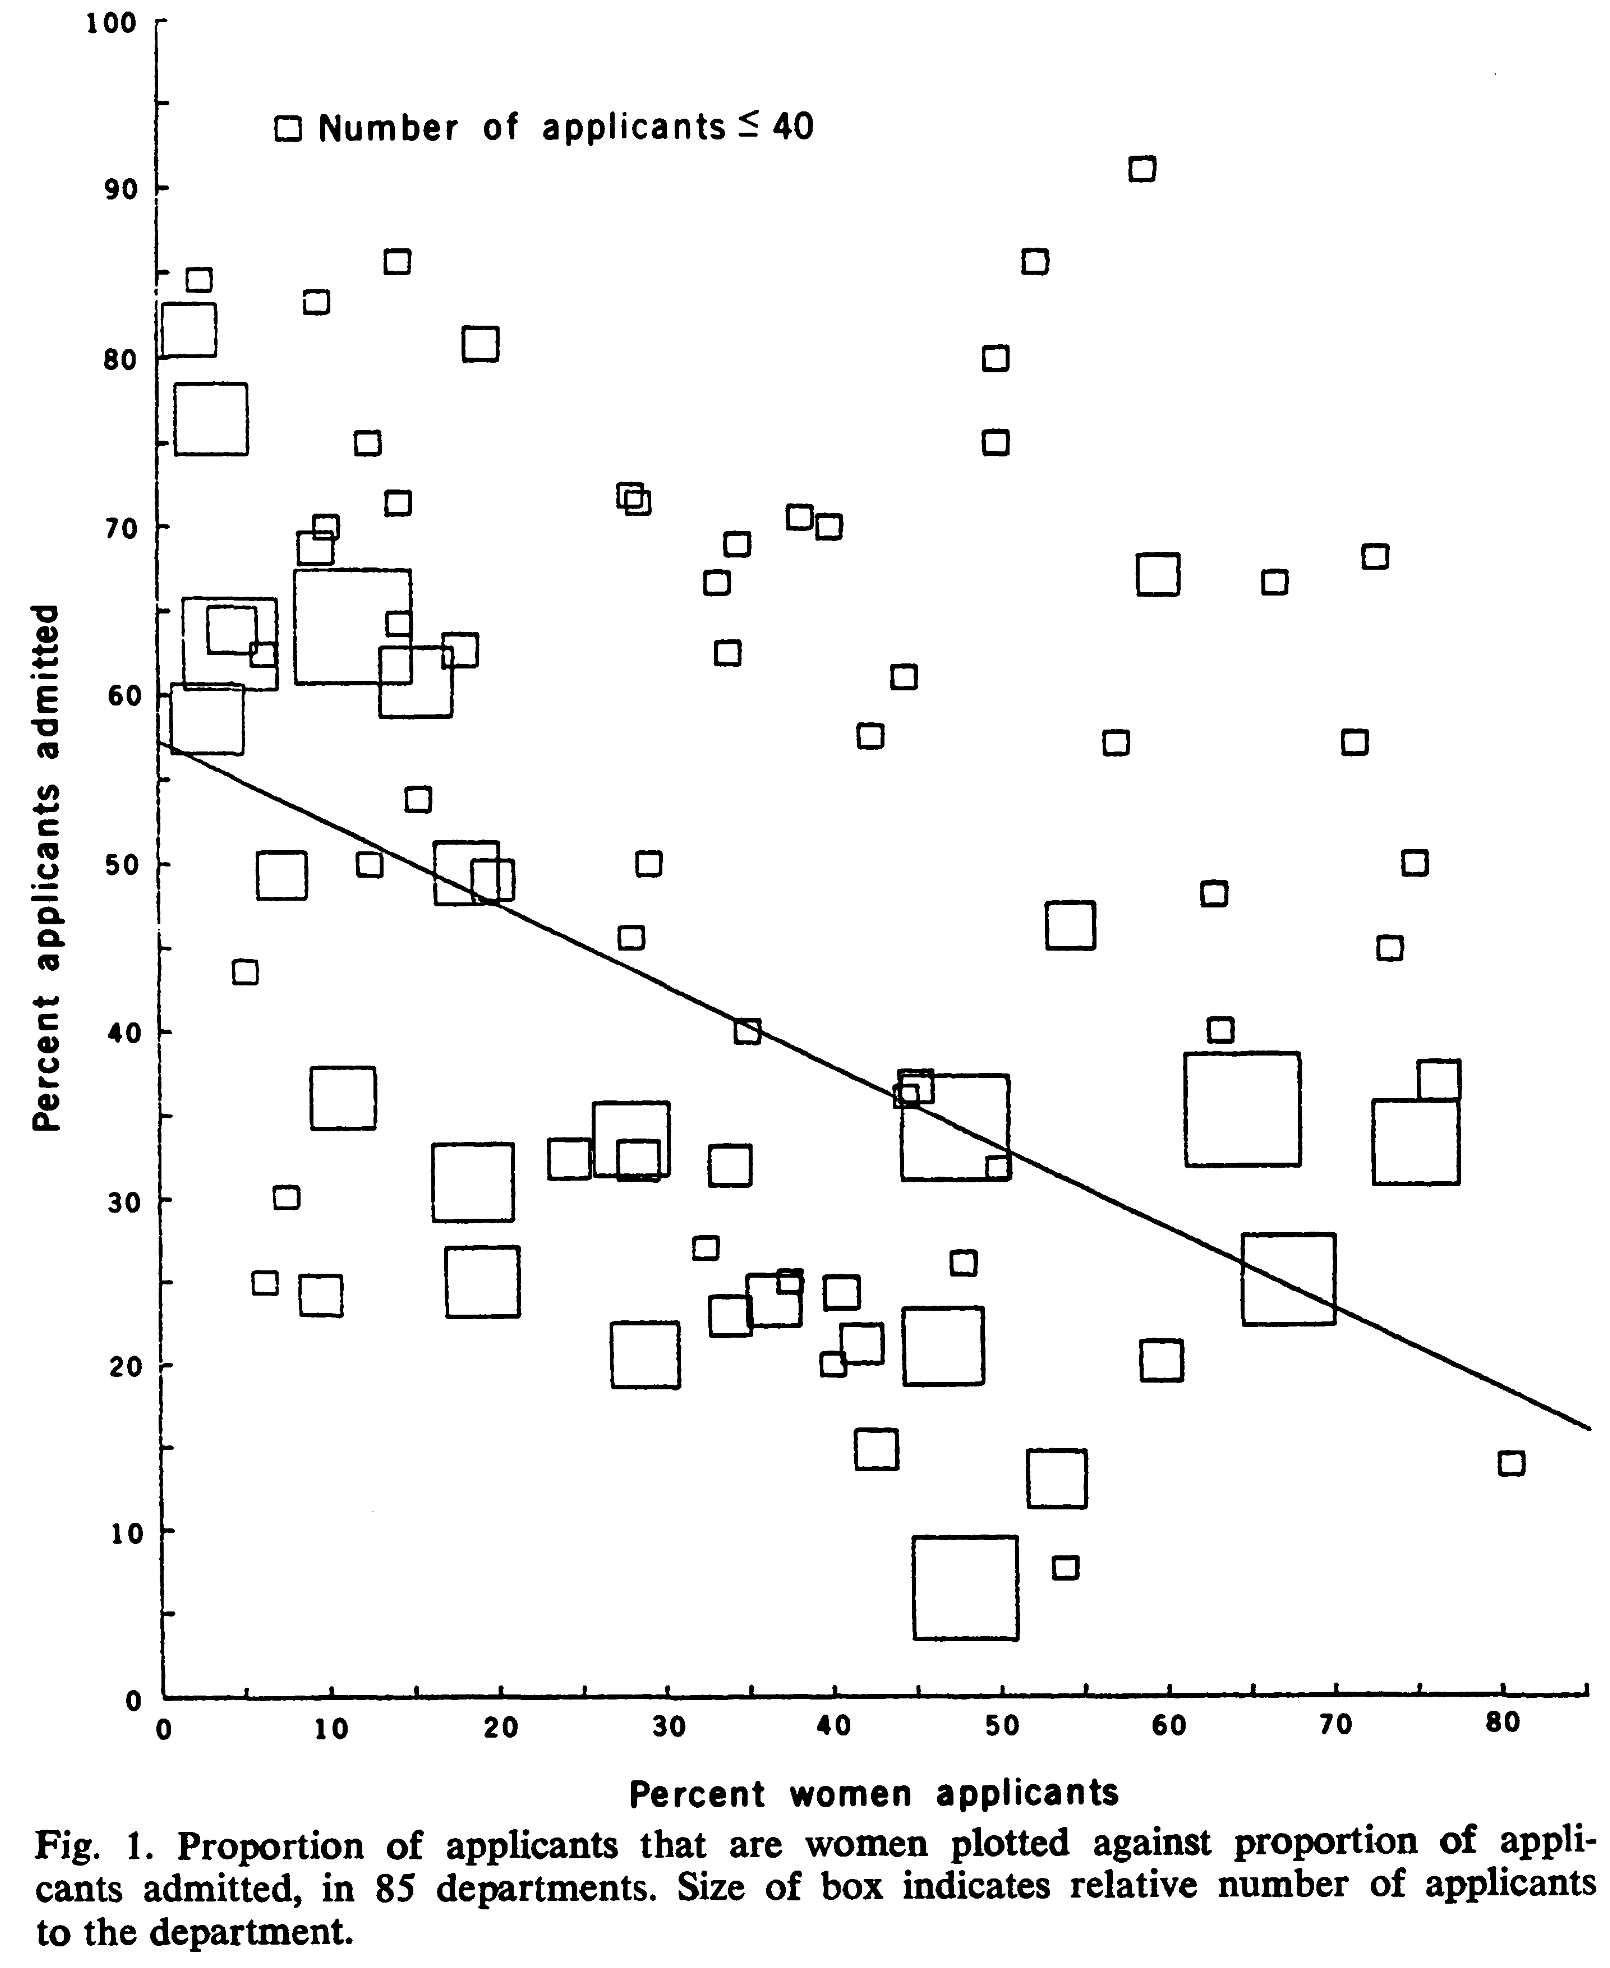
\includegraphics[width=0.6\textwidth,height=\textheight]{fig/berkley.png}
\caption{\label{fig:berkley} Graph taken from \citet[page 403]{Bickel1975Sex}}
\end{figure}

Here you can read the summary of their infamous study:

\begin{quote}
``Examination of aggregate data on graduate admissions to the University of California, Berkeley, for fall 1973 shows a clear but misleading pattern of bias against female applicants. Examination of the disaggregated data reveals few decision-making units that show statistically significant departures from expected frequencies of female admissions, and about as many units appear to favor women as to favor men. If the data are properly pooled, taking into account the autonomy of departmental decision making, thus correcting for the tendency of women to apply to graduate departments that are more difficult for applicants of either sex to enter, there is a small but statistically significant bias in favor of women. The graduate departments that are easier to enter tend to be those that require more mathematics in the undergraduate preparatory curriculum. The bias in the aggregated data stems not from any pattern of discrimination on the part of admissions committees, which seem quite fair on the whole, but apparently from prior screening at earlier levels of the educational system. Women are shunted by their socialization and education toward fields of graduate study that are generally more crowded, less productive of completed degrees, and less well funded, and that frequently offer poorer professional employment prospects.''
\end{quote}

\begin{exercise}
\protect\hypertarget{exr:graduateadmission}{}\label{exr:graduateadmission}Graduate admissions

Read the first three pages of \citet{Bickel1975Sex}, i.e., pages 398-400, and answer the following questions. The article can be found \href{https://www.science.org/doi/pdf/10.1126/science.187.4175.398}{here}.

\begin{enumerate}
\def\labelenumi{\alph{enumi})}
\tightlist
\item
  Describe the two assumptions that must be true in order to prove that UC Berkeley discriminates against women or men overall.
\item
  Table 1, shows that 277 fewer women and 277 more men were admitted than we would have expected under the two assumptions. Show how this number was calculated.
\item
  Explain the analogy with fish that illustrates the danger of pooling data.
\end{enumerate}

Please find solution to the exercise \protect\hyperlink{sol:graduateadmission}{in the appendix.}
\end{exercise}

\begin{exercise}
\protect\hypertarget{exr:simpsonpara}{}\label{exr:simpsonpara}Simpson's Paradox

\begin{enumerate}
\def\labelenumi{\arabic{enumi}.}
\tightlist
\item
  What is Simpson's Paradox?

  \begin{enumerate}
  \def\labelenumii{\alph{enumii})}
  \tightlist
  \item
    A phenomenon in which the direction of a relationship between two variables changes when a third variable is introduced
  \item
    A phenomenon in which the strength of a relationship between two variables changes when a third variable is introduced
  \item
    The phenomenon where correlation appears to be present in different groups of data, but disappears or reverses when the groups are combined
  \end{enumerate}
\item
  What is a potential cause of Simpson's Paradox?

  \begin{enumerate}
  \def\labelenumii{\alph{enumii})}
  \tightlist
  \item
    Differences in the variance of the two variables
  \item
    Differences in the correlation of the two variables
  \item
    Confounding variables
  \item
    Differences in the sample size of the two variables
  \end{enumerate}
\end{enumerate}

Please find solution to the exercise \protect\hyperlink{sol:simpsonpara}{here}
\end{exercise}

\hypertarget{rubin-causal-model}{%
\subsection{Rubin causal model}\label{rubin-causal-model}}

\begin{quote}
\citet[page 314]{Keele2015statistics}: \emph{``An identification analysis identifies the assumptions needed for statistical estimates to be given a causal interpretation.''}
\end{quote}

If we are interested in the causal effect of a certain treatment on an outcome, we need to compare the outcome of the individuals who received the treatment to the outcome of the individuals who did not receive the treatment. However, if the counterfactual outcome is missing for some individuals, we cannot make this comparison and therefore cannot estimate the causal effect. Unfortunately, the counterfactual is usually non-existing.
For example, if we want to measure the effect of a vaccine we never can have a person who is vaccinated and not vaccinated at the same time. Formally, we have either \(Y_i(1)\) or \(Y_i(1)\), where \(Y_i\) denotes the effect/output of individual \(i\) in case of being vaccinated (1) and not vaccinated (0).

Thus, the so-called individual treatment effect (ITE) does not exist for person \(i\):
\[
ITE_i=Y_i(1)-Y_i(0)
\]

The Rubin Causal Model, also known as the potential outcomes framework, is a statistical framework for analyzing causality in the context of missing data.
Table \ref{tab:tab21} is taken from \citet{Neal2020Introduction} and shows some example data to illustrate that the fundamental problem of causal inference is actually a missing data problem.
The Model goes back to Donald B. Rubin (*1943) a statistician and is now a widely used method for causal inference. The basic premise of the Rubin Causal Model is that for each individual in a study, there are two potential outcomes: the outcome that would occur if the individual were exposed to a certain treatment or intervention (the ``treatment group''), and the outcome that would occur if the individual were not exposed to that treatment (the ``control group''). The key idea is that these potential outcomes can be used to infer causality by comparing the outcomes between the treatment and control groups even if we do not have a full set of data.

\begin{longtable}[]{@{}cccccc@{}}
\caption{\label{tab:tab21} Example data to illustrate that the fundamental problem of causal inference}\tabularnewline
\toprule()
i & T & Y & Y(1) & Y(0) & Y(1)-Y(0) \\
\midrule()
\endfirsthead
\toprule()
i & T & Y & Y(1) & Y(0) & Y(1)-Y(0) \\
\midrule()
\endhead
1 & 0 & 0 & ? & 0 & ? \\
2 & 1 & 1 & 1 & ? & ? \\
3 & 1 & 0 & 0 & ? & ? \\
4 & 0 & 0 & ? & 0 & ? \\
5 & 0 & 1 & ? & 1 & ? \\
6 & 1 & 1 & 1 & ? & ? \\
\bottomrule()
\end{longtable}

\begin{figure}
\centering
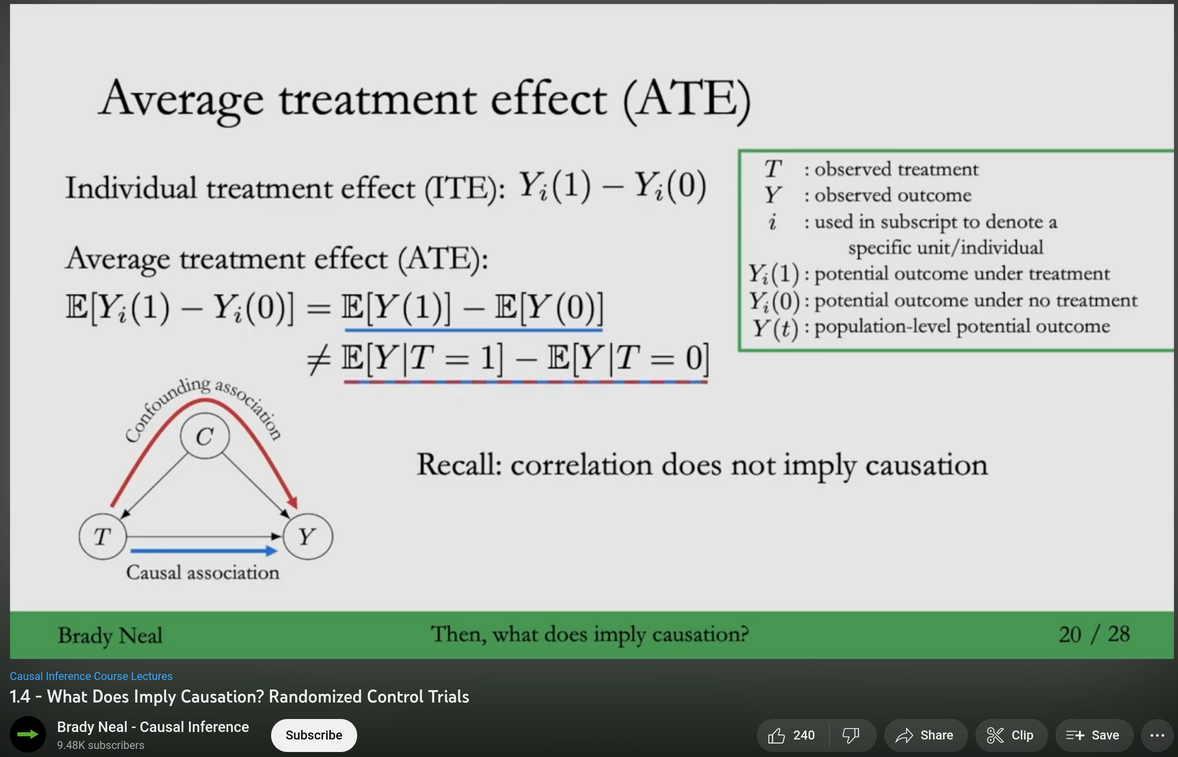
\includegraphics[width=0.5\textwidth,height=\textheight]{fig/neal-rct.png}
\caption[\label{fig:nealrct} Average treatment effect (ATE)]{\label{fig:nealrct} Average treatment effect (ATE)\footnotemark{}}
\end{figure}
\footnotetext{Picture is taken from \url{https://youtu.be/gGaWU8XEoGk}}

Watch the video of Brady Neal's lecture \href{https://youtu.be/gGaWU8XEoGk}{\emph{What Does Imply Causation? Randomized Control Trials}}. Alternatively, you can read \href{https://www.bradyneal.com/Introduction_to_Causal_Inference-Dec17_2020-Neal.pdf}{chapter 2} of his lecture notes \citep{Neal2020Introduction}.

Under certain assumptions, the Rubin Causal Model allows for the estimation of the Average Treatment Effect (ATE), which is the difference in the expected outcomes between the treatment and control groups, given by the formula:
\[
ATE\triangleq \mathbb{E}[Y(1)-Y(0)]
\]

There are several ways to estimate the ATE under the Rubin Causal Model some of which will be part of this course. Applied correctly, it can provide valuable insights into causality and inform decision making. However, the Rubin Causal Model has its limitations and assumptions that need to be met in order for the inferences to be valid.

To get the average treatment effect (ATE) we can take the average of the individual treatment effects (ITE):
\begin{equation}
  ATE\triangleq \mathbb{E}[Y(1)-Y(0)] = \mathbb{E} [\underbrace{Y_i(1)-Y_i(0)}_{ITE}]
\label{eq:feq}
\end{equation}

\hypertarget{its-difficult-to-overcome-the-fundamental-problem}{%
\section{Its difficult to overcome the fundamental problem}\label{its-difficult-to-overcome-the-fundamental-problem}}

In the following we will discuss conditions that need to hold in order to empirically draw causal conclusions from the ATE without bias. This is important because equation \eqref{eq:feq} does very often not hold when using observational data.

\hypertarget{ignorability}{%
\subsection{Ignorability}\label{ignorability}}

Refering to table \ref{tab:tab21}, Brady \citet{Neal2020Introduction} wrote:

\begin{quote}
\emph{``what makes it valid to calculate the ATE by taking the average of the Y(0) column, ignoring the question marks, and subtracting that from the average of the Y(1) column, ignoring the question marks?'' This ignoring of the question marks (missing data) is known as ignorability. Assuming ignorability is like ignoring how people ended up selecting the treatment they selected and just assuming they were randomly assigned their treatment''} \citep[p.~9]{Neal2020Introduction}
\end{quote}

Randomized controlled trials (RCTs) are characterized by randomly assigning individuals to different treatment groups and comparing the outcomes of those groups. Thus, they are build on the assumption of \emph{ignorability}
\[
(Y(1), Y(0)) \perp T
\]
which allows to write the ATE as follows:
\begin{align}
\mathbb{E}[Y(1)]-\mathbb{E}[Y(0)] & =\mathbb{E}[Y(1) \mid T=1]-\mathbb{E}[Y(0) \mid T=0] \\
& =\mathbb{E}[Y \mid T=1]-\mathbb{E}[Y \mid T=0].\label{eq:feq2}
\end{align}

Another perspective on this assumption is the concept of exchangeability. Exchangeability refers to the idea that the treatment groups can be interchanged such that if they were switched, the new treatment group would have the same outcomes as the old treatment group, and the new control group would have the same outcomes as the old control group.

\hypertarget{unconfoundedness}{%
\subsection{Unconfoundedness}\label{unconfoundedness}}

While randomized controlled trials (RCTs) assume the concept of ignoreability, most observational data present challenges in drawing causal conclusions due to the presence of confounding factors that affect both (1) the likelihood of individuals being part of the treatment group and (2) the observed outcome. For instance, regional factors can affect both the number of storks and the number of babies born in a region. These factors are typically referred to as confounders, which we discussed in section \ref{cornotcaus} as having the potential to create the illusion of a causal impact where none exists. However, empirical methods are available \emph{to control for} these confounders and prevent the violation of the ignoreability assumption.

\begin{exercise}
\protect\hypertarget{exr:treatmenteffects}{}\label{exr:treatmenteffects}Treatment effects

Read sections 2.1 and 2.3 of \citet{Neal2020Introduction}.

\begin{enumerate}
\def\labelenumi{\arabic{enumi}.}
\tightlist
\item
  What is the individual treatment effect (ITE)?
\item
  What is the average treatment effect (ATE)?
\item
  How is the ATE calculated?
\item
  Can the ATE be used to determine the effect of a treatment on an individual level?
\item
  What are some potential sources of bias when estimating the ATE?
\end{enumerate}

Please find solution to the exercise \protect\hyperlink{sol:treatmenteffects}{in the appendix.}
\end{exercise}

\hypertarget{statistics}{%
\chapter{Statistics}\label{statistics}}

\hypertarget{sampling}{%
\section{Sampling}\label{sampling}}

In this chapter, we learn\ldots{}

\begin{itemize}
\tightlist
\item
  \ldots{} what characterizes a \emph{good} sample, i.e., a sample that can be used for empirical analysis using statistical inference.
\item
  \ldots{} to distinguish between a sample and a population.
\item
  \ldots{} to identify biased samples.
\item
  \ldots{} to distinguish between random sampling and random assignment.
\item
  \ldots{} that a simple random sample is the gold standard because of its properties.
\item
  \ldots{} different ways to collect data and draw a sample, respectively (stratification, clustering, opportunity)
\end{itemize}

\hypertarget{the-hite-report}{%
\subsection{The Hite Report}\label{the-hite-report}}

In 1976, when the \emph{The Hite Report} \citep[see][]{Hite1976Hite} was published it instantly became a best seller.
Hite used an individualistic research method. Thousands of responses from anonymous questionnaires were used as a framework to develop a discourse on human responses to gender and sexuality. The following comic concludes the main results.

\begin{figure}
\centering

\includegraphics[width=0.25\textwidth,height=\textheight]{fig/hite.jpeg}
\caption{\label{fig:hitereport} The Hite Report}
\end{figure}

\begin{figure}
\centering
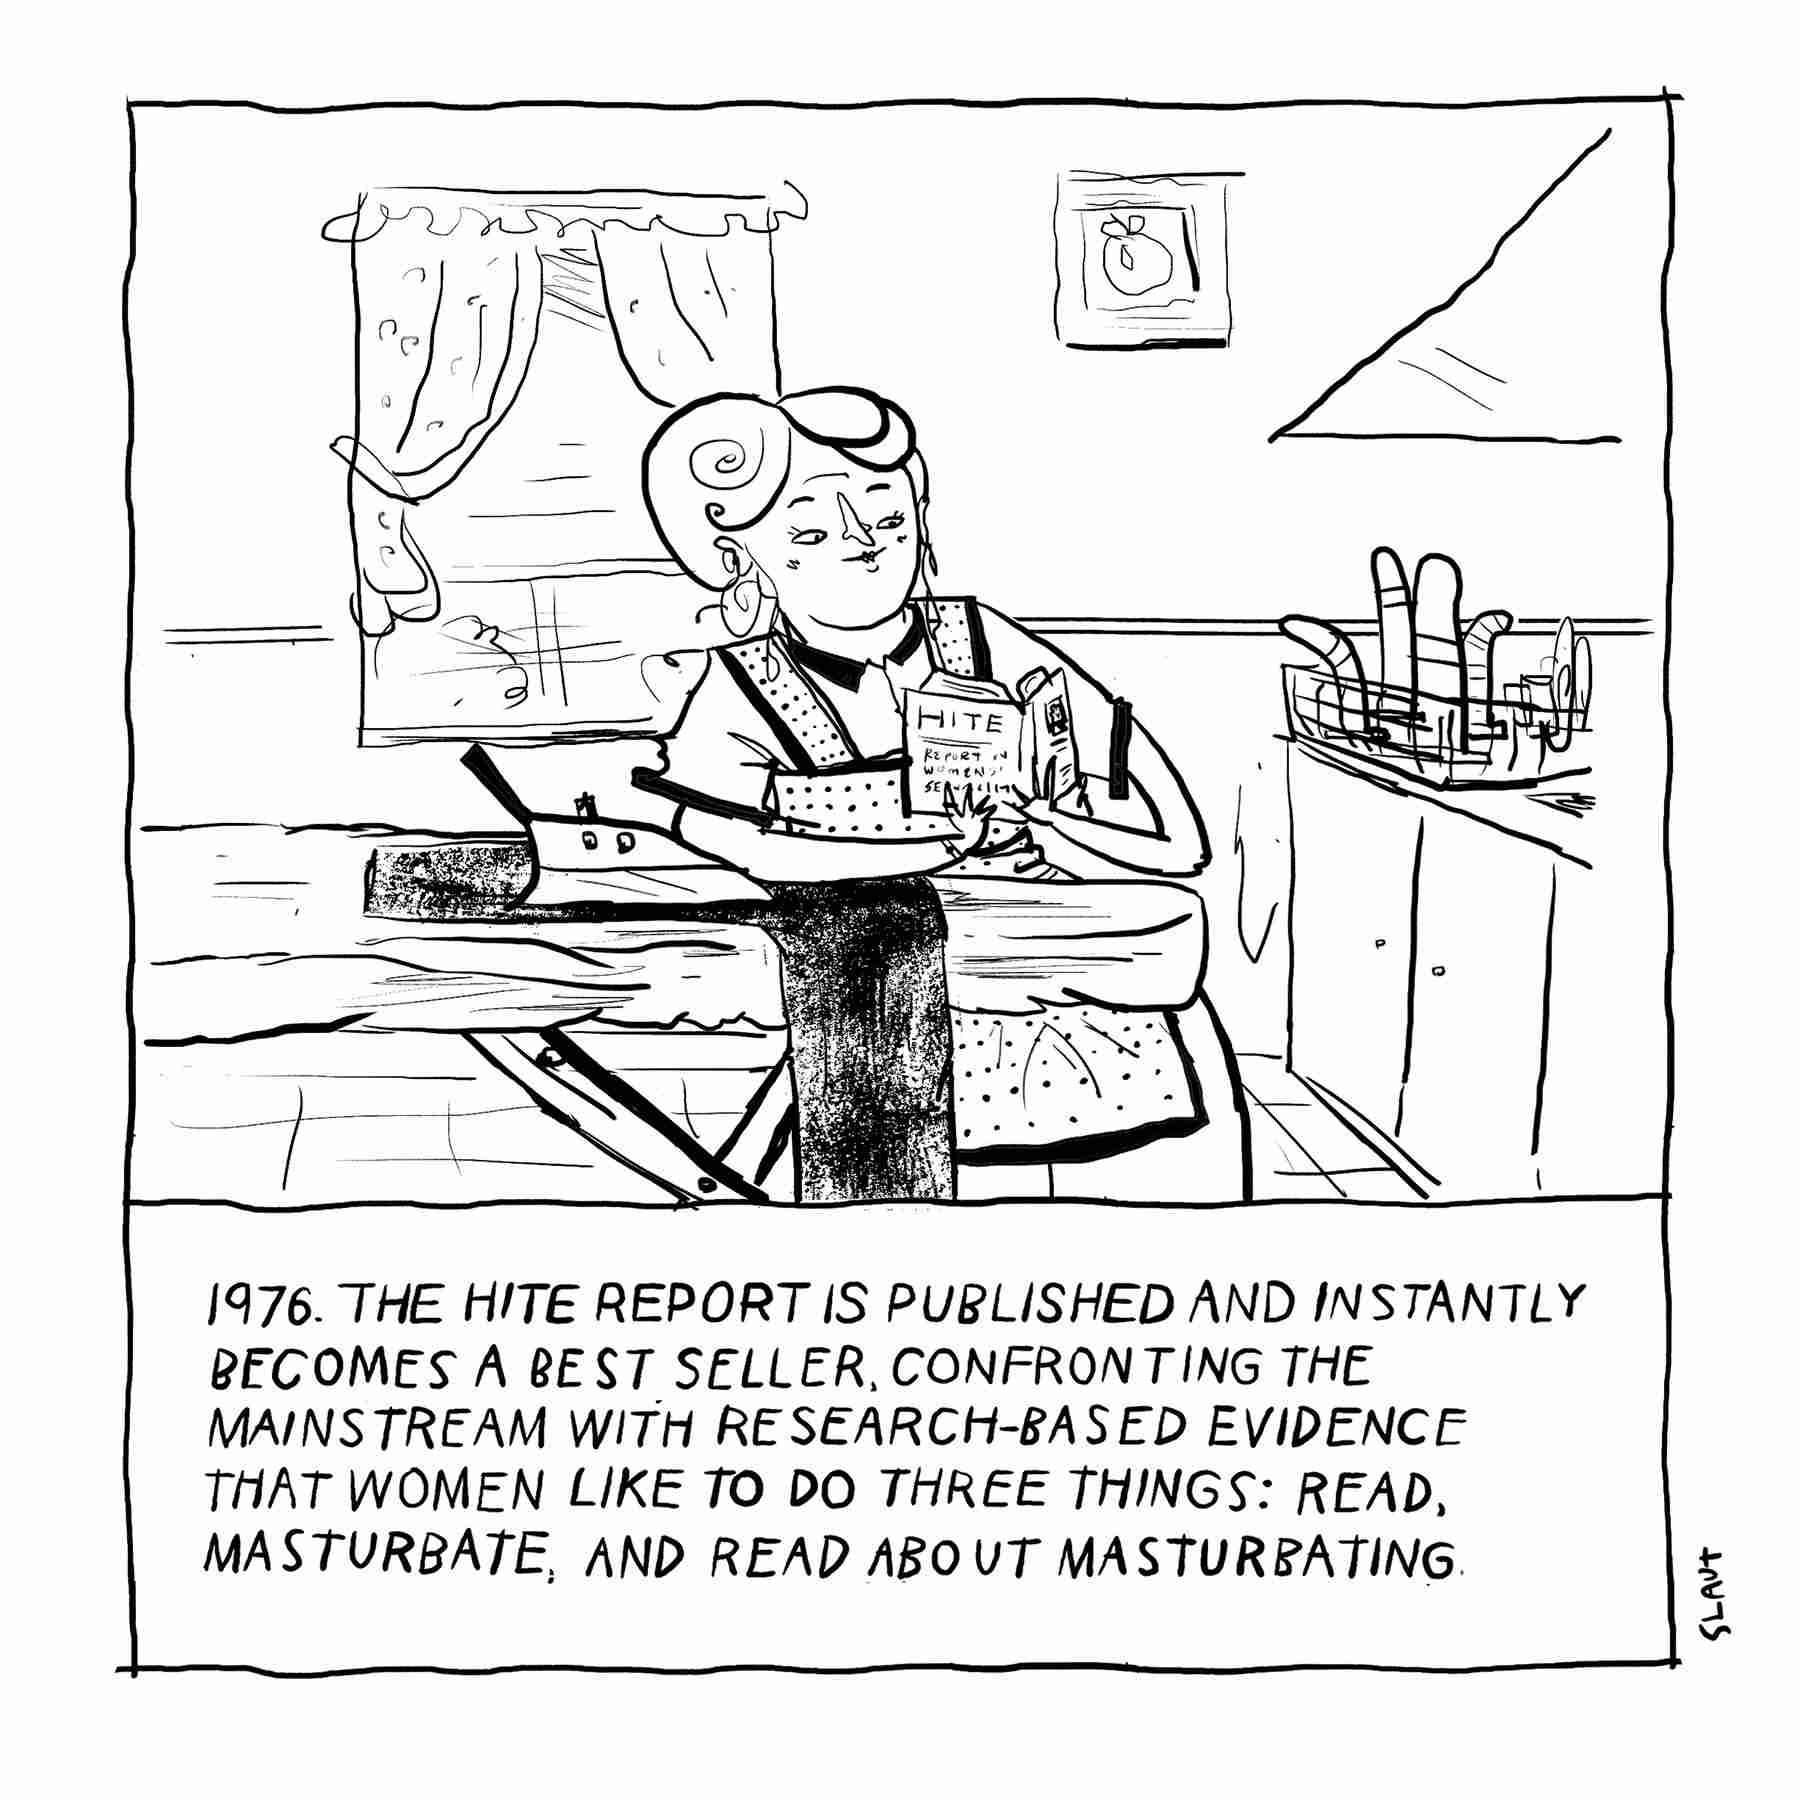
\includegraphics[width=0.75\textwidth,height=\textheight]{fig/hitereport.jpg}
\caption[\label{fig:hitedo} Comic on the Hite Report]{\label{fig:hitedo} Comic on the Hite Report\footnotemark{}}
\end{figure}
\footnotetext{Picture is taken from www.theparisreview.org/blog/2017/07/21/great-moments-literacy-hite-report}

The picture of womens' sexuality in \citet{Hite1976Hite} was probably a bit biased as the sample can hardly be considered to be a \textbf{random and unbiased} one:

\begin{itemize}
\tightlist
\item
  Less than 5\% of all questionnaires which were sent out were filled out and returned (response bias).
\item
  The questions were only sent out to women's organizations (an opportunity sample).
\end{itemize}

Thus, the results were based on a sample of women who were highly motivated to answer survey's questions, for whatever reason.

\hypertarget{sample-design}{%
\subsection{Sample design}\label{sample-design}}

In statistics and quantitative research methodology, a sample is a group of individuals or objects that are collected or selected from a statistical population using a defined procedure. The elements of a sample are called sample points, sampling units, or observations.

Usually, the population is very large, and therefore, conducting a census or complete enumeration of all individuals in the population is either impractical or impossible. Therefore, a sample is taken to represent a manageable subset of the population. Data is collected from the sample, and statistics are calculated to make inferences or extrapolations from the sample to the population.

In statistics, we often rely on a \textbf{sample}, that is, a small subset of a larger set of
data, to draw inferences about the larger set. The larger set is known as the
\textbf{population} from which the sample is drawn.

Researchers adopt a variety of sampling strategies. The most straightforward is
\textbf{simple random sampling}. Such sampling requires every member of the population
to have an equal chance of being selected into the sample. In addition, the selection
of one member must be independent of the selection of every other member. That
is, picking one member from the population must not increase or decrease the
probability of picking any other member (relative to the others). In this sense, we
can say that simple random sampling chooses a sample by pure chance. To check
your understanding of simple random sampling, consider the following example.
What is the population? What is the sample? Was the sample picked by simple
random sampling? Is it biased?

\hypertarget{random-sampling}{%
\subsubsection{Random sampling}\label{random-sampling}}

Random sampling is a sampling procedure by which each member of a population has an equal chance of being included in the sample. Random sampling ensures a representative sample. There are several types of random sampling. In simple random sampling, not only each item in the population but each sample has an equal probability of being picked. In systematic sampling, items are selected from the population at uniform intervals of time, order, or space (as in picking every one-hundredth name from a telephone directory). Systematic sampling can be biased easily, such as, for example, when the amount of household garbage is measured on Mondays (which includes the weekend garbage). In stratified and cluster sampling, the population is divided into strata (such as age groups) and clusters (such as blocks of a city) and then a proportionate number of elements is picked at random from each stratum and cluster. Stratified sampling is used when the variations within each stratum are small in relation to the variations between strata. Cluster sampling is used when the opposite is the case. In what follows, we assume simple random sampling. Sampling can be from a finite population (as in picking cards from a deck without replacement) or from an infinite population (as in picking parts produced by a continuous process or cards from a deck with replacement).

In statistics, a \textbf{simple random sample} is a subset of individuals (a sample) chosen from a larger set (a population). Each individual is chosen randomly and entirely by chance, such that each individual has the same probability of being chosen at any stage during the sampling process, and each subset of k individuals has the same probability of being chosen for the sample as any other subset of k individuals.

The simple random sample has two important properties:

\begin{enumerate}
\def\labelenumi{\arabic{enumi}.}
\tightlist
\item
  \textbf{UNBIASED:} Each unit has the same chance of being chosen.
\item
  \textbf{INDEPENDENCE:} Selection of one unit has no influence on the selection of other units.
\end{enumerate}

\begin{exercise}
\protect\hypertarget{exr:randomsampling}{}\label{exr:randomsampling}Random sampling

\begin{itemize}
\tightlist
\item
  What is meant by random sampling (simple random sample)?
\item
  What is its importance?
\item
  Why is having a large sample always better than having a small(er) one?
\end{itemize}

Please find solution to the exercise \protect\hyperlink{sol:randomsampling}{here.}
\end{exercise}

\begin{exercise}
\protect\hypertarget{exr:examplesampleerror}{}\label{exr:examplesampleerror}Examples of sample errors

Watch \href{https://creativemaths.net/videos/video-variation-sources}{Sampling error and variation} and read the following examples:

\textbf{Example 1:} You have been hired by the National Election Commission to
examine how the American people feel about the fairness of the voting procedures in the U.S. Who will you ask?

It is not practical to ask every single American how he or she feels about the
fairness of the voting procedures. Instead, we query a relatively small number of
Americans, and draw inferences about the entire country from their responses. The
Americans actually queried constitute our sample of the larger population of all
Americans. The mathematical procedures whereby we convert information about
the sample into intelligent guesses about the population fall under the rubric of
inferential statistics.
A sample is typically a small subset of the population. In the case of voting
attitudes, we would sample a few thousand Americans drawn from the hundreds of
millions that make up the country. In choosing a sample, it is therefore crucial that
it not over-represent one kind of citizen at the expense of others. For example,
something would be wrong with our sample if it happened to be made up entirely
of Florida residents. If the sample held only Floridians, it could not be used to infer
the attitudes of other Americans. The same problem would arise if the sample were
comprised only of Republicans. \_\_Inferential statistics are based on the assumption
that sampling is random\}. We trust a random sample to represent different segments
of society in close to the appropriate proportions (provided the sample is large
enough; see below).

\textbf{Example 2:} We are interested in examining how many math classes have
been taken on average by current graduating seniors at American colleges
and universities during their four years in school. Whereas our population in
the last example included all US citizens, now it involves just the graduating
seniors throughout the country. This is still a large set since there are
thousands of colleges and universities, each enrolling many students. It would be
prohibitively costly to examine the transcript of every college senior. We
therefore take a sample of college seniors and then make inferences to the
ntire population based on what we find. To make the sample, we might first
choose some public and private colleges and universities across the United
States. Then we might sample 50 students from each of these institutions.
Suppose that the average number of math classes taken by the people in our
sample were 3.2. Then we might speculate that 3.2 approximates the number
we would find if we had the resources to examine every senior in the entire
population. But we must \textbf{be careful about the possibility that our sample is
non-representative of the population}. Perhaps we chose an overabundance of
math majors, or chose too many technical institutions that have heavy math
requirements. Such bad sampling makes our sample unrepresentative of the
population of all seniors.
To solidify your understanding of sampling bias, consider the following
example. Try to identify the population and the sample, and then reflect on
whether the sample is likely to yield the information desired.

\textbf{Example 3:} A substitute teacher wants to know how students in the class
did on their last test. The teacher asks the 10 students sitting in the front row
to state their latest test score. He concludes from their report that the class
did extremely well. What is the sample? What is the population? Can you
identify any problems with choosing the sample in the way that the teacher
did?

In Example 3, the population consists of all students in the class. The sample is
made up of just the 10 students sitting in the front row. \textbf{The sample is not likely to
be representative of the population}. Those who sit in the front row tend to be more
interested in the class and tend to perform higher on tests. Hence, the sample may
perform at a higher level than the population.

\textbf{Example 4:} A coach is interested in how many cartwheels the average
college freshmen at his university can do. Eight volunteers from the
freshman class step forward. After observing their performance, the coach
concludes that college freshmen can do an average of 16 cartwheels in a row
without stopping.

In Example 4, the population is the class of all freshmen at the coach's university.
The sample is composed of the 8 volunteers. The sample is poorly chosen because
\textbf{volunteers are more likely to be able to do cartwheels} than the average freshman;
people who can't do cartwheels probably did not volunteer! In the example, we are
also not told of the gender of the volunteers. Were they all women, for example?
That might affect the outcome, contributing to the non-representative nature of the
sample.

\textbf{Example 5:}
Sometimes it is not feasible to build a sample using simple random sampling. To
see the problem, consider the fact that both Dallas and Houston are competing to
be hosts of the 2012 Olympics. Imagine that you are hired to assess whether most
Texans prefer Houston to Dallas as the host, or the reverse. Given the
impracticality of obtaining the opinion of every single Texan, you must construct a
sample of the Texas population. But now notice how difficult it would be to
proceed by simple random sampling. For example, how will you contact those
individuals who don't vote and don't have a phone? Even among people you find
in the telephone book, how can you identify those who have just relocated to
California (and had no reason to inform you of their move)? What do you do about
the fact that since the beginning of the study, an additional 4,212 people took up
residence in the state of Texas? As you can see, it is sometimes very difficult to
develop a truly random procedure.
\end{exercise}

\hypertarget{other-sampling-methods}{%
\subsubsection{Other sampling methods}\label{other-sampling-methods}}

\textbf{Systematic sampling}

Systematic sampling (a.k.a. interval sampling) relies on arranging the study population according to some ordering scheme and then selecting elements at regular intervals through that ordered list. Systematic sampling involves a random start and then proceeds with the selection of every k\(^{th}\) element from then onwards.

\textbf{Accidental sampling / opportunity sampling / convenience sampling}

These sampling methods describe a type of nonprobability sampling which involves the sample being drawn from that part of the population which is close to hand. That is, a population is selected because it is readily available and convenient.

\textbf{Stratified sampling}

Since simple random sampling often does not ensure a representative sample, a
sampling method called stratified random sampling is sometimes used to make the
sample more representative of the population. This method can be used if the
population has a number of distinct groups. In stratified sampling, you
first identify members of your sample who belong to each group. Then you
randomly sample from each of those subgroups in such a way that the sizes of the
subgroups in the sample are proportional to their sizes in the population.
Let`s take an example: Suppose you were interested in views of capital
punishment at an urban university. You have the time and resources to interview
200 students. The student body is diverse with respect to age; many older people
work during the day and enroll in night courses (average age is 39), while younger
students generally enroll in day classes (average age of 19). It is possible that night
students have different views about capital punishment than day students. If 70\%
of the students were day students, it makes sense to ensure that 70\% of the sample
consisted of day students. Thus, your sample of 200 students would consist of 140
day students and 60 night students. The proportion of day students in the sample
and in the population (the entire university) would be the same. Inferences to the
entire population of students at the university would therefore be more secure.

\textbf{Cluster sampling}

Sometimes it is more cost-effective to select respondents in groups (clusters) of similar respondents. Sampling is often clustered by geography, or by time periods.

\hypertarget{random-assignment}{%
\subsubsection{Random assignment}\label{random-assignment}}

In experimental research, populations are often hypothetical. For example, in an
experiment comparing the effectiveness of a new anti-depressant drug with a
placebo, there is no actual population of individuals taking the drug. In this case, a
specified population of people with some degree of depression is defined and a
random sample is taken from this population. The sample is then randomly divided
into two groups; one group is assigned to the treatment condition (drug) and the
other group is assigned to the control condition (placebo). This random division of
the sample into two groups is called random assignment. \textbf{Random assignment is
critical for the validity of an experiment}. For example, consider the bias that could
be introduced if the first 20 subjects to show up at the experiment were assigned to
the experimental group and the second 20 subjects were assigned to the control
group. It is possible that subjects who show up late tend to be more depressed than
those who show up early, thus making the experimental group less depressed than
the control group even before the treatment was administered.
In experimental research of this kind, failure to assign subjects randomly to
groups is generally more serious than having a non-random sample. Failure to
randomize (the former error) invalidates the experimental findings. A non-random
sample (the latter error) simply restricts the generalizability of the results.

\hypertarget{sample-size-matters}{%
\subsection{Sample size matters}\label{sample-size-matters}}

The sample size is an important feature of any empirical study in which the goal is to make inferences about a population from a sample. In practice, the sample size used in a study is usually determined based on the cost, time, or convenience of collecting the data, and the need for it to offer sufficient statistical power.

Recall that the definition of a random sample is a sample in which every member of the population has an equal chance of being selected. This means that the \textbf{sampling procedure} rather than the \textbf{results} of the procedure define what it means for a sample to be random. Random samples, especially if the sample size is small, are not necessarily representative of the entire population.

Larger sample sizes generally lead to increased precision when estimating unknown parameters. For example, if we wish to know the proportion of a certain species of fish that is infected with a pathogen, we would generally have a more precise estimate of this proportion if we sampled and examined 200 rather than 100 fish. Several fundamental facts of mathematical statistics describe this phenomenon, including the \emph{law of large numbers} and the \emph{central limit theorem}.

A helpful slogan to keep in mind while scrutinizing statistical results is ``garbage in, garbage out''. Regardless of how scientifically sound and visually appealing a statistic may appear, the formula used to derive it is oblivious to the quality of the data that underpins it. It is your responsibility to conduct a thorough examination. For example, if the data on which the statisitc is based emanates from a biased sample (one that favors certain individuals over others), a flawed design, unreliable data-collection protocols, or misleading questions, the margin of error becomes \emph{bad}. If the bias is sufficiently severe, the outcomes become worthless.

\hypertarget{descriptive-statistics}{%
\section{Descriptive statistics}\label{descriptive-statistics}}

\hypertarget{univariate-data}{%
\subsection{Univariate data}\label{univariate-data}}

\hypertarget{arithmetic-mean}{%
\subsubsection{Arithmetic mean}\label{arithmetic-mean}}

The arithmetic mean (\(\bar{x}\)) is calculated as the sum of all the values in a dataset divided by the total number of values:

\[
\bar{x} = \frac{{\sum_{i=1}^{n} x_i}}{n}
\]

where \(\bar{x}\) represents the arithmetic mean, \(x_i\) represents each individual value in the dataset, and \(n\) represents the total number of values in the dataset.

\hypertarget{median}{%
\subsubsection{Median}\label{median}}

The median is the middle value of a dataset when it is sorted in ascending or descending order. If the dataset has an odd number of values, the median is the middle value. If the dataset has an even number of values, the median is the average of the two middle values.

\hypertarget{mode}{%
\subsubsection{Mode}\label{mode}}

The mode is the value or values that appear most frequently in a dataset.

\hypertarget{range}{%
\subsubsection{Range}\label{range}}

The range is the difference between the maximum and minimum values in a dataset.

\[
\text{{Range}} = \max(x_i) - \min(x_i)
\]

where \(\text{{Range}}\) represents the range value, and \(x_i\) represents each individual value in the dataset.

\hypertarget{variance}{%
\subsubsection{Variance}\label{variance}}

The variance represents the average of the squared deviations of a random variable from its mean. It quantifies the extent to which a set of numbers deviates from their average value. Variance is commonly denoted as \(Var(X)\), \(\sigma^2\), or \(s^2\). The calculation of variance is as follows:
\[
\sigma^2={\frac{1}{n}}\sum _{i=1}^{n}(x_{i}-\mu )^{2}
\]
However, it is better to use
\[
\sigma^2={\frac{1}{n-1}}\sum _{i=1}^{n}(x_{i}-\mu )^{2}.
\]

The use of \(n - 1\) instead of \(n\) in the formula for the sample variance is known as \emph{Bessel's correction}, which corrects the bias in the estimation of the population variance, and some, but not all of the bias in the estimation of the population standard deviation.
Consequently this way to calculate the variance and hence the standard deviation is called the \emph{sample standard deviation} or the \emph{unbiased estimation of standard deviation}.
In other words, when working with a sample instead of the full population the limited number of observations tend to be closer to the \emph{sample mean} than to the \emph{population mean}, see figure \ref{fig:bessel}. Bessels Correction takes that into account.

For a detailed explanation, you can watch the video by \href{https://youtu.be/sHRBg6BhKjI}{StatQuest with Josh Starmer: Why Dividing By N Underestimates the Variance}

\begin{figure}
\centering
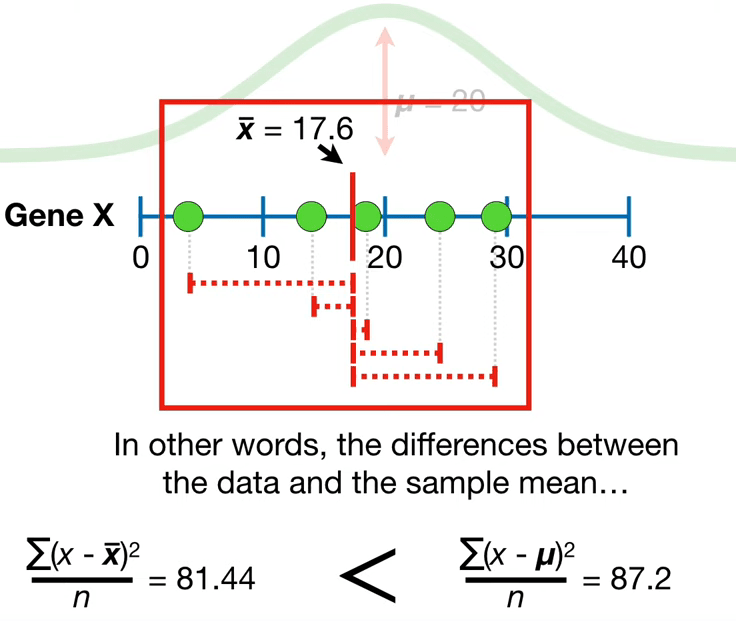
\includegraphics[width=0.75\textwidth,height=\textheight]{fig/bessel.png}
\caption[\label{fig:bessel} Bias when using the sample mean]{\label{fig:bessel} Bias when using the sample mean\footnotemark{}}
\end{figure}
\footnotetext{Picture is taken from the video \url{https://youtu.be/sHRBg6BhKjI}}

\hypertarget{standard-deviation}{%
\subsubsection{Standard deviation}\label{standard-deviation}}

As the variance is hard to interpret, the standard deviation is a more often used measure of dispersion.
A low standard deviation indicates that the values tend to be close to the mean.
It is often abbreviated with \(sd\), \(SD\), or most often with the Greek letter sigma, \(\sigma\).
The underlying idea is to measure the average deviation from the mean.
It is calculated as follows:
\[
sd(x)=\sqrt{\sigma^2}={\sqrt {{\frac {1}{n-1}}\sum _{i=1}^{n}\left(x_{i}-{\mu}\right)^{2}}}=\sigma
\]

\hypertarget{standard-error}{%
\subsubsection{Standard error}\label{standard-error}}

The standard deviation (SD) measures the amount of variability, or dispersion, for a subject set of data from the mean, while the standard error of the mean (SEM) measures how far the sample mean of the data is likely to be from the true population mean. The SEM is always smaller than the SD. It matters because it helps you estimate how well your sample data represents the whole population.

The standard error of the mean (SEM) can be expressed as:
\[
sd(\bar{x})=\sigma_{\bar {x}}\ = s = {\frac {\sigma }{\sqrt {n}}}
\]
where \(\sigma\) is the standard deviation of the population and \(n\) is the size (number of observations) of the sample.

Also see the video by \href{https://youtu.be/A82brFpdr9g}{StatQuest with Josh Starmer: Standard Deviation vs Standard Error, Clearly Explained!!!}

\hypertarget{why-divide-by-the-square-root-of-n}{%
\subparagraph*{\texorpdfstring{Why divide by the square root of \(n\)?}{Why divide by the square root of n?}}\label{why-divide-by-the-square-root-of-n}}

Let \(X_{i}\) be an independent draw from a distribution with mean \(\bar{x}\) and variance \(\sigma^{2}\).
What is the variance of \(\bar{x}\)?

By definition:
\[
\operatorname{Var}(x)=E\left[\left(x_{i}-E\left[x_{i}\right]\right)^{2}\right]=\sigma^{2}
\]
so
\begin{align*}
\operatorname{Var}(\bar{x})&=E\left[\left(\frac{\sum x_{i}}{n}-E \left[\frac{\sum x_{i}}{n}\right]\right)^{2}\right]\\
&=E\left[\left(\frac{\sum x_{i}}{n}-\frac{1}{n} E\left[ \sum x_{i}\right]\right)^{2}\right]\\
&=\frac{1}{n^{2}} E\left[\left(\sum x_{i}-E\left[\sum x_{i}\right]\right)^{2}\right]\\
&=\frac{1}{n^{2}} E\left[\left(\sum x_{i}- \sum \bar{x}\right)^{2}\right]\\
&=\frac{1}{n^{2}} E\left[(x_{1}+x_{2}+\cdots+x_{n}-\underbrace{\bar{x}-\bar{x}-\cdots -\bar{x}}_{n \text{ terms }})^{2}\right]\\
&=\frac{1}{n^{2}} E\left[\sum\left(x_{i}-\bar{x}\right)^{2}\right]\\
&=\frac{1}{n^{2}} \sum E\left(x_{i}-\bar{x}\right)^{2}\\
&=\frac{1}{n^{2}} \underbrace{\sum \sigma^{2}}_{n\cdot \sigma^{2}}\\
&=\frac{1}{n} \sigma^{2}
\end{align*}
and hence
\[
sd(\bar x)=\sqrt{\operatorname{Var}(\bar{x})}=s={\frac {\sigma }{\sqrt {n}}}
\]

\hypertarget{coefficient-of-variation}{%
\subsubsection{Coefficient of variation}\label{coefficient-of-variation}}

The coefficient of variation (\(CoV\)) is a relative measure of variability and is calculated as the ratio of the standard deviation to the mean, expressed as a percentage:

\[
CoV =  \frac{\sigma}{\bar{x}}
\]

where \(CoV\) represents the coefficient of variation, \(\sigma\) represents the standard deviation, and \(\bar{x}\) represents the arithmetic mean.

\hypertarget{skewness}{%
\subsubsection{Skewness}\label{skewness}}

Skewness is a measure of the asymmetry of a distribution. There are different formulas to calculate skewness, but one common method is using the third standardized moment (\(\gamma_1\)):

\[
\gamma_1 = \frac{{\sum_{i=1}^{n} \left(\frac{x_i - \bar{x}}{\sigma}\right)^3}}{n}
\]

where \(\gamma_1\) represents the skewness, \(x_i\) represents each individual value in the dataset, \(\bar{x}\) represents the arithmetic mean, \(\sigma\) represents the standard deviation, and \(n\) represents the total number of values in the dataset.

\hypertarget{kurtosis}{%
\subsubsection{Kurtosis}\label{kurtosis}}

Kurtosis measures the peakedness or flatness of a probability distribution. There are different formulations for kurtosis, and one of the common ones is the fourth standardized moment. The formula for kurtosis is given by:

\[
\text{{Kurtosis}} = \frac{{\frac{1}{n} \sum_{i=1}^{n}(x_i - \bar{x})^4}}{{\left(\frac{1}{n} \sum_{i=1}^{n}(x_i - \bar{x})^2\right)^2}}
\]

where \(\text{Kurtosis}\) represents the kurtosis value, \(x_i\) represents each individual value in the dataset, \(\bar{x}\) represents the mean of the dataset, and \(n\) represents the total number of values in the dataset.

\hypertarget{bivariate-data}{%
\subsection{Bivariate data}\label{bivariate-data}}

\hypertarget{covariance}{%
\subsubsection{Covariance}\label{covariance}}

Covariance \(Cov(X,Y)\) (or \(\sigma_{XY}\)) is a measure of the joint variability of two variables (\(x\) and \(y\)) and their observations \(i\), respectively.
The covariance is positive when larger values of one variable tend to correspond with larger values of the other variable, or when smaller values of one variable tend to correspond with smaller values of the other variable. On the other hand, a negative covariance suggests an inverse relationship, where larger values of one variable tend to correspond with smaller values of the other variable.

It's important to note that the magnitude of the covariance is influenced by the units of measurement, making it challenging to interpret directly. Additionally, the spread of the variables also affects the covariance.
The formula for calculating covariance is as follows:
\[
\operatorname{Cov}(X,Y)=\sigma_{XY}={\frac {1}{n-1}}\sum _{i=1}^{n}(x_{i}-\bar{x})(y_{i}-\bar{y})
\]
where \(cov(X,Y)\) represents the covariance, \(\sigma_{XY}\) is an alternative notation, \(x_i\) and \(y_i\) are the individual observations of variables \(X\) and \(Y\), \(\bar{x}\) and \(\bar{y}\) are the means of variables \(X\) and \(Y\), and \(n\) is the total number of observations.

To gain a better understanding of the concept and calculation of covariance, I highly recommend watching Josh Starmer's informative and visually engaging video titled \href{https://youtu.be/qtaqvPAeEJY}{Covariance and Correlation Part 1: Covariance}.

\hypertarget{the-correlation-coefficient-bravais-pearson}{%
\subsubsection{The correlation coefficient (Bravais-Pearson)}\label{the-correlation-coefficient-bravais-pearson}}

The Pearson correlation coefficient measures the linear relationship between two variables. It is calculated as the covariance of the variables divided by the product of their standard deviations.
\[
\rho_{X,Y} = \frac{{\text{Cov}(X, Y)}}{{\sigma_X \sigma_Y}}
\]

where \(\rho\) represents the Pearson correlation coefficient, \(\text{Cov}(X, Y)\) denotes the covariance between variables \(X\) and \(Y\), \(\sigma_X\) denotes the standard deviation of variable \(X\), and \(\sigma_Y\) denotes the standard deviation of variable \(Y\). It has a value between +1 and -1.

By dividing the covariance of \(X\) and \(Y\) by the multiplication of the standard deviations of \(X\) and \(Y\), the correlation coefficient is normalized by having a minimum of -1 and a maximum of 1. Thus, it can fix the problem of the variance that the scale (unit of measurement) determines the size of the variance.

I highly recommend watching the video \href{https://youtu.be/xZ_z8KWkhXE}{Pearson's Correlation, Clearly Explained!!!}
StatQuest with Josh Starmer. It provides a clear and engaging explanation of the meaning of correlation. The video features informative animations that help visualize the concept.

In interpreting correlations, it is important to remember that they\ldots{}

\begin{enumerate}
\def\labelenumi{\arabic{enumi}.}
\tightlist
\item
  \ldots{} only reflect the strength and direction of linear relationships,
\item
  \ldots{} do not provide information about the slope of the relationship, and
\item
  \ldots{} fail to explain important aspects of nonlinear relationships.
\end{enumerate}

\begin{figure}

{\centering 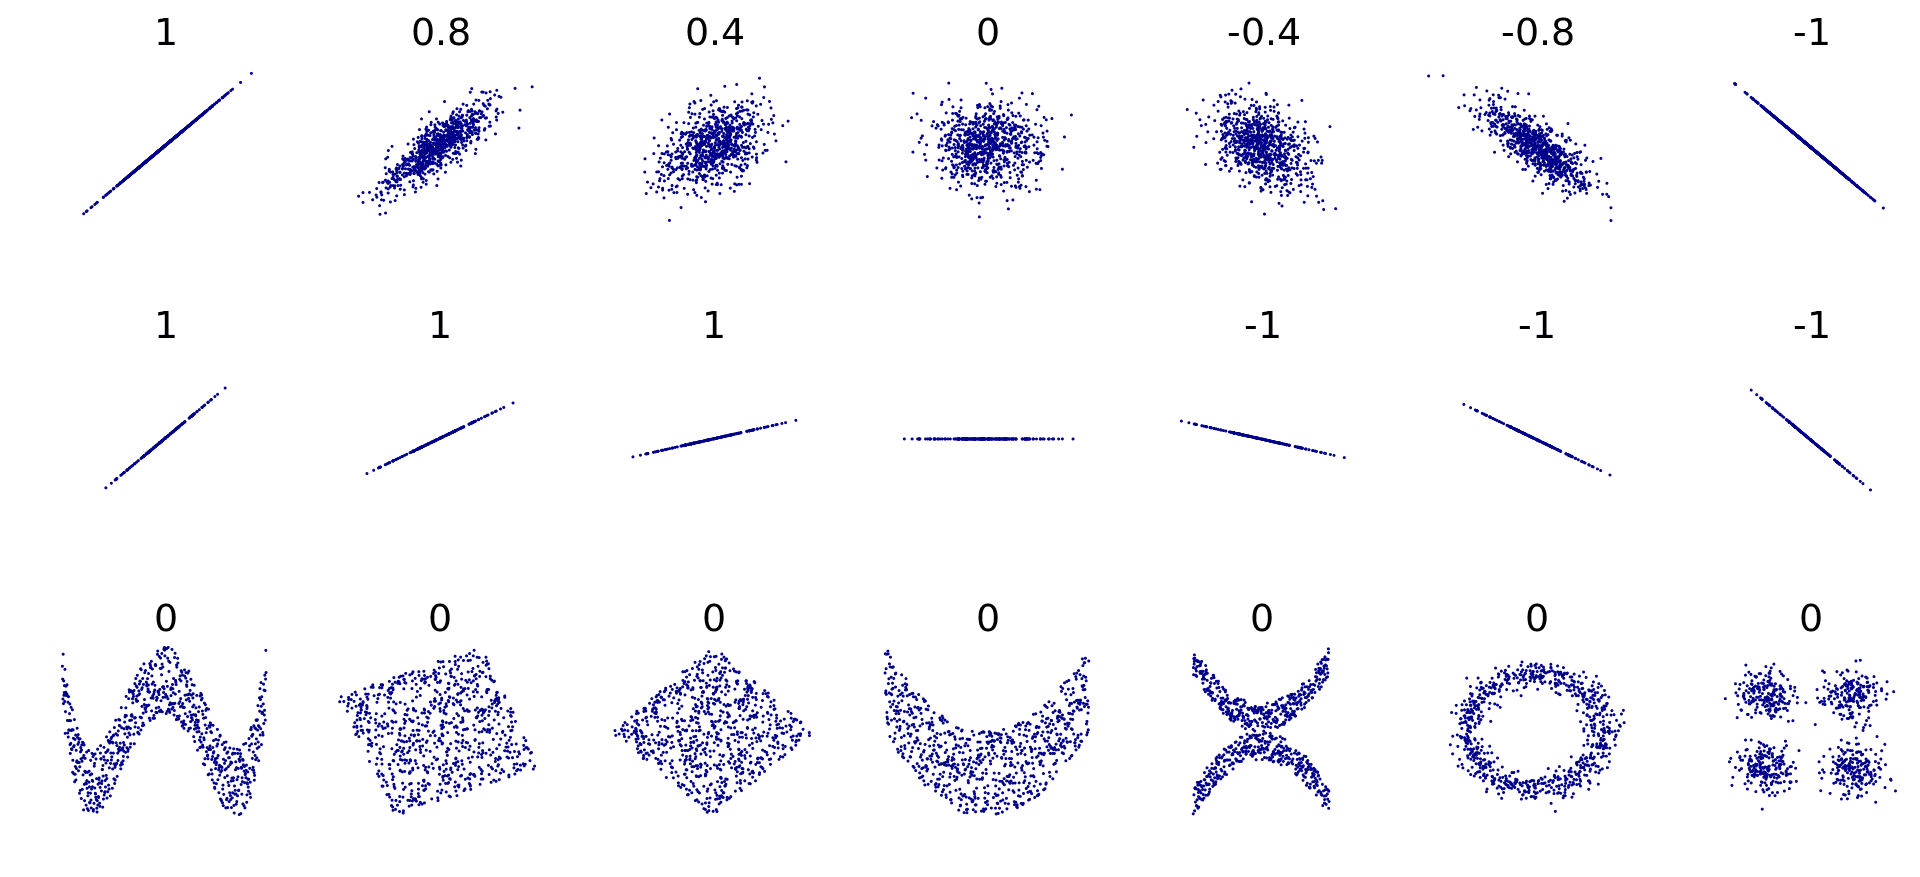
\includegraphics[width=0.75\linewidth]{fig/corelate_overview} 

}

\caption{Correlations are blind on some eye}\label{fig:corelateoverview}
\end{figure}

Figure \ref{fig:corelateoverview} shows that correlation coefficients are limited in to explaining the relationship of two variables.
For example, when the slope of a relationship is zero, the correlation coefficient becomes undefined due to the variance of \(Y\) being zero.
Furthermore, Pearson's correlation coefficient is sensitive to outliers, and all correlation coefficients are prone to sample selection biases. It is crucial to be careful when attempting to correlate two variables, particularly when one represents a part and the other represents the total.
It is also worth noting that small correlation values do not necessarily indicate a lack of association between variables. For example, Pearson's correlation coefficient can underestimates the association between variables exhibiting a quadratic relationship. Therefore, it is always advisable to examine scatterplots in conjunction with correlation analysis.

In figure \ref{fig:allcorsame} you see various graphs that all have the same correlation coefficient and share other statistical properties like is investigated in exercise \ref{exr:Datasaurus}.

\begin{figure}

{\centering 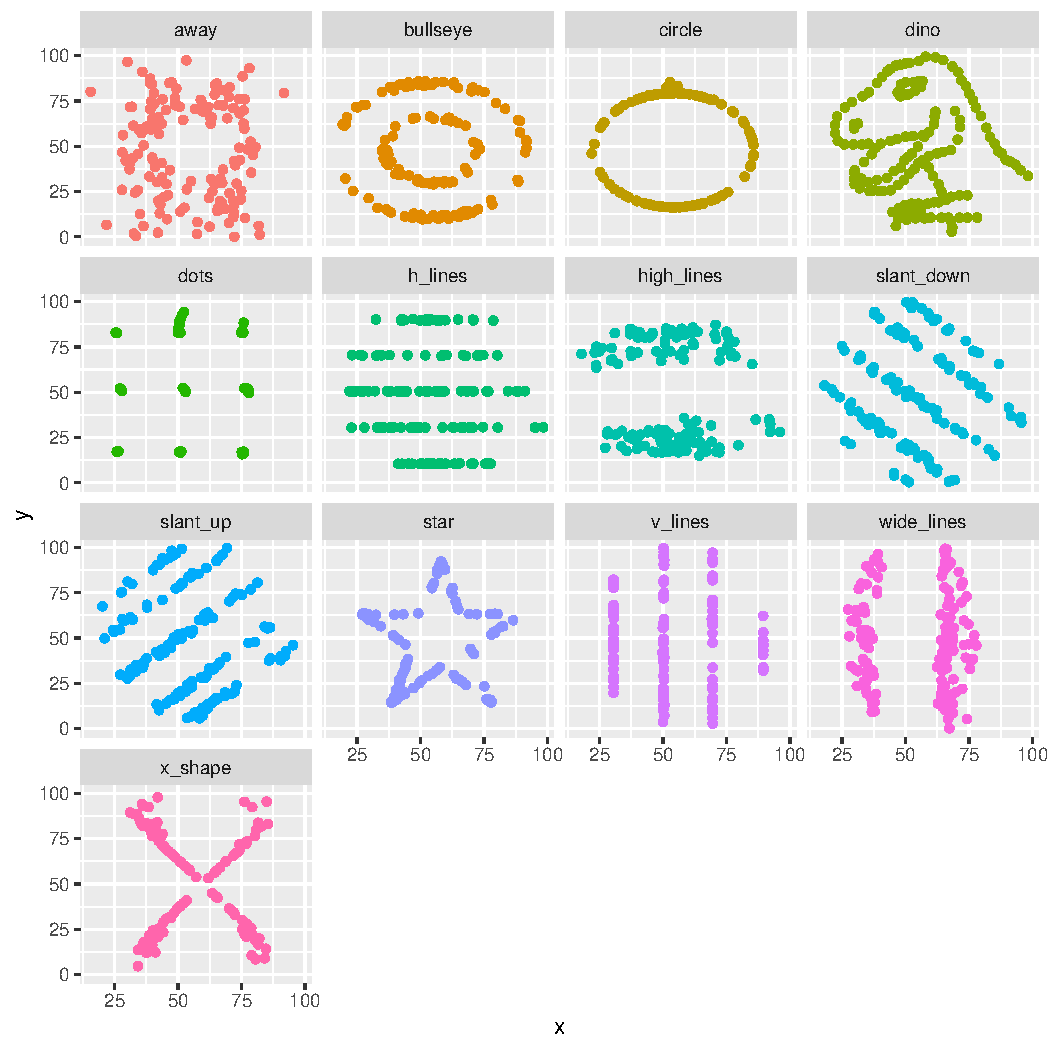
\includegraphics{fig/allcorsame} 

}

\caption{These diagrams all have the same statistical properties\protect\footnotemark}\label{fig:allcorsame}
\end{figure}
\footnotetext{This graph was produced employing the `datasauRus` R package.}

\hypertarget{rank-correlation-coefficient-spearman}{%
\subsubsection{Rank correlation coefficient (Spearman)}\label{rank-correlation-coefficient-spearman}}

Spearman's rank correlation coefficient is a measure of the strength and direction of the monotonic relationship between two variables.
It can be calculated for a sample of size \(n\) by converting the \(n\) raw scores \(X_i, Y_i\) to ranks \(\text{R}(X_i), \text{R}(Y_i)\), then using the following formula:

\[
r_s = \rho_{\operatorname{R}(X),\operatorname{R}(Y)} = \frac{\text{cov}(\operatorname{R}(X), \operatorname{R}(Y))}{\sigma_{\operatorname{R}(X)} \sigma_{\operatorname{R}(Y)}},
\]

where
\(\rho\) denotes the usual Pearson correlation coefficient, but applied to the rank variables,
\(\operatorname{cov}(\operatorname{R}(X), \operatorname{R}(Y))\) is the covariance of the rank variables,
\(\sigma_{\operatorname{R}(X)}\) and \(\sigma_{\operatorname{R}(Y)}\) are the standard deviations of the rank variables.

If all \(n\) ranks are distinct integers, you can use the handy formula:

\[
\rho = 1 - \frac{6\sum d_i^2}{n(n^2 - 1)}
\]

where \(\rho\) denotes the correlation coefficient, \(\sum d_i^2\) is the sum of squared differences between the ranks of corresponding pairs of variables, and \(n\) represents the number of pairs of observations.

The coefficient ranges from -1 to 1. A value of 1 indicates a perfect increasing monotonic relationship, while a value of -1 indicates a perfect decreasing monotonic relationship. A value of 0 suggests no monotonic relationship between the variables.

Spearman's rank correlation coefficient is a non-parametric measure and is often used when the relationship between variables is not linear or when the data is in the form of ranks or ordinal categories.

\begin{exercise}
\protect\hypertarget{exr:Datasaurus}{}\label{exr:Datasaurus}

Datasaurus

\begin{enumerate}
\def\labelenumi{\alph{enumi})}
\tightlist
\item
  Load the packages \texttt{datasauRus} and \texttt{tidyverse}. If necessary, install these packages.
\end{enumerate}

\end{exercise}

\begin{enumerate}
\def\labelenumi{\alph{enumi})}
\setcounter{enumi}{1}
\item
  The package\texttt{datasauRus} comes with a dataset in two different formats: \texttt{datasaurus\_dozen} and \texttt{datasaurus\_dozen\_wide}. Store them as \texttt{ds} and \texttt{ds\_wide}.
\item
  Open and read the R vignette of the \texttt{datasauRus} package. Also open the R documentation of the dataset \texttt{datasaurus\_dozen}.
\item
  Explore the dataset: What are the dimensions of this dataset? Look at the descriptive statistics.
\item
  How many unique values does the variable \texttt{dataset} of the tibble \texttt{ds} have? Hint: The function unique() return the unique values of a variable and the function length() returns the length of a vector, such as the unique elements.
\item
  Compute the mean values of the \texttt{x} and \texttt{y} variables for each entry in \texttt{dataset}. Hint: Use the group\_by() function to group the data by the appropriate column and then the summarise() function to calculate the mean.
\item
  Compute the standard deviation, the correlation, and the median in the same way. Round the numbers.
\item
  What can you conclude?
\item
  Plot all datasets of \texttt{ds}. Hide the legend. Hint: Use the \texttt{facet\_wrap()} and the \texttt{theme()} function.
\item
  Create a loop that generates separate scatter plots for each unique datatset of the tibble \texttt{ds}. Export each graph as a png file.
\item
  Watch the video \href{https://youtu.be/T-kxUB29t0o}{Animating the Datasaurus Dozen Dataset in R} from The Data Digest on YouTube.
\end{enumerate}

Please find the solutions \href{https://htmlpreview.github.io/?https://raw.githubusercontent.com/hubchev/hubchev.github.io/main/various/datasaurus_solution.html}{here}.

\begin{exercise}
\protect\hypertarget{exr:summarystatistics}{}\label{exr:summarystatistics}Summary statistics

Calculate for the following datasets: the mode, the median, the 20\% quantile, the range, the interquartile range, the variance, the arithmetic mean, the sample standard deviation, the coefficient of variation.

\begin{enumerate}
\def\labelenumi{\alph{enumi})}
\tightlist
\item
  For ten participants in a scientific conference the age
  has been noted: \[25, 21, 18, 37, 56, 89, 46, 23, 21, 34.\]
\item
  A random sample of 128 visitors of the Cupcake festival yielded the following frequencies regarding the cupcake consumption during their visit:
\end{enumerate}

\begin{longtable}[]{@{}lrrrrrr@{}}
\toprule()
Cupcages consumed & 1 & 2 & 3 & 4 & 5 & 6 \\
\midrule()
\endhead
Abs. freq. & 2 & 30 & 37 & 28 & 23 & 8 \\
\bottomrule()
\end{longtable}

Please find solution to the exercise \protect\hyperlink{sol:summarystatistics}{here.}
\end{exercise}

\begin{exercise}
\protect\hypertarget{exr:destatexcel}{}\label{exr:destatexcel}Summary statistics in spreadsheet software

Given is the following datset: \[0, 0, 40, 50, 50, 60, 70, 90, 100, 100.\]
Compute the following summary statistics of the data set using a spreadsheet software like \textit{Excel} or \textit{LibreOffice Calc}:
mean, median, mode, quartiles (Q1, Q2, Q3), range, interquartile range, variance, standard deviation, mean absolute deviation, coefficient of variation and skewness.

Please find solution to the exercise \protect\hyperlink{sol:destatexcel}{here.}
\end{exercise}

\begin{exercise}
\protect\hypertarget{exr:guessstat}{}\label{exr:guessstat}Guess the summary statistics

Given are the following variables:

\begin{longtable}[]{@{}rrrrr@{}}
\toprule()
a & b & c & d & e \\
\midrule()
\endhead
97 & 70 & 1 & 1 & 970 \\
98 & 80 & 50 & 2 & 980 \\
99 & 90 & 50 & 3 & 990 \\
100 & 100 & 50 & 4 & 1000 \\
101 & 110 & 50 & 5 & 1010 \\
102 & 120 & 50 & 6 & 1020 \\
103 & 130 & 99 & 7 & 1030 \\
\bottomrule()
\end{longtable}

Rank the variables without calculating concrete numbers accordingly to the values of the following descriptive statistics: mode, median, mean, range, variance, standard deviation, coefficient of variation.

Please find solution to the exercise \protect\hyperlink{sol:guessstat}{here.}
\end{exercise}

\hypertarget{simple-linear-regression}{%
\subsection{Simple linear regression}\label{simple-linear-regression}}

The linear regression analysis is a widely used technique for predictive modeling. Its purpose is to establish a mathematical equation that relates a continuous response variable, denoted as \(y\), to one or more independent variables, represented by \(x\). The objective is to create a regression model that enables the prediction of the value of \(y\) based on known values of \(x\).

To ensure meaningful predictions, it is important to have an adequate number of observations, denoted as \(i\), available for the variables of interest.

The linear regression model can be expressed as:
\[
y_i = \beta_{0} + \beta_{1} x_i + \epsilon_i,
\]
where the index \(i\) denotes the individual observations, ranging from \(i = 1\) to \(n\). The variable \(y_i\) represents the dependent variable, also known as the regressand. The variable \(x_i\) represents the independent variable, also referred to as the regressor. \(\beta_0\) denotes the intercept of the population regression line, a.k.a. the constant. \(\beta_1\) denotes the slope of the population regression line. Lastly, \(\epsilon_i\) refers to the error term or the residual, which accounts for the deviation between the predicted and observed values of \(y_i\).

By fitting a linear regression model, one aims to estimate the values of \(\beta_0\) and \(\beta_1\) in order to obtain an equation that best captures the relationship between \(y\) and \(x\).

While the correlation coefficient and the slope in simple linear regression are similar in many ways, it's important to note that they are not identical. The correlation coefficient measures the strength and direction of the linear relationship between variables in a broader sense, while the slope in simple linear regression specifically quantifies the change in the dependent variable associated with a unit change in the independent variable.

\hypertarget{estimating-the-coefficients-of-the-linear-regression-model}{%
\subsubsection{Estimating the coefficients of the linear regression model}\label{estimating-the-coefficients-of-the-linear-regression-model}}

In practice, the intercept and slope of the regression are unknown. Therefore, we must employ data to estimate the unknown parameters, \(\beta_0\) and \(\beta_1\).
The method we use is called the ordinary least squared (OLS) method. The idea is to minimize the sum of the squared differences of all \(y_i\) and \(y_i^*\) as sketched in figure \ref{fig:regressionols}.

\begin{figure}
\centering
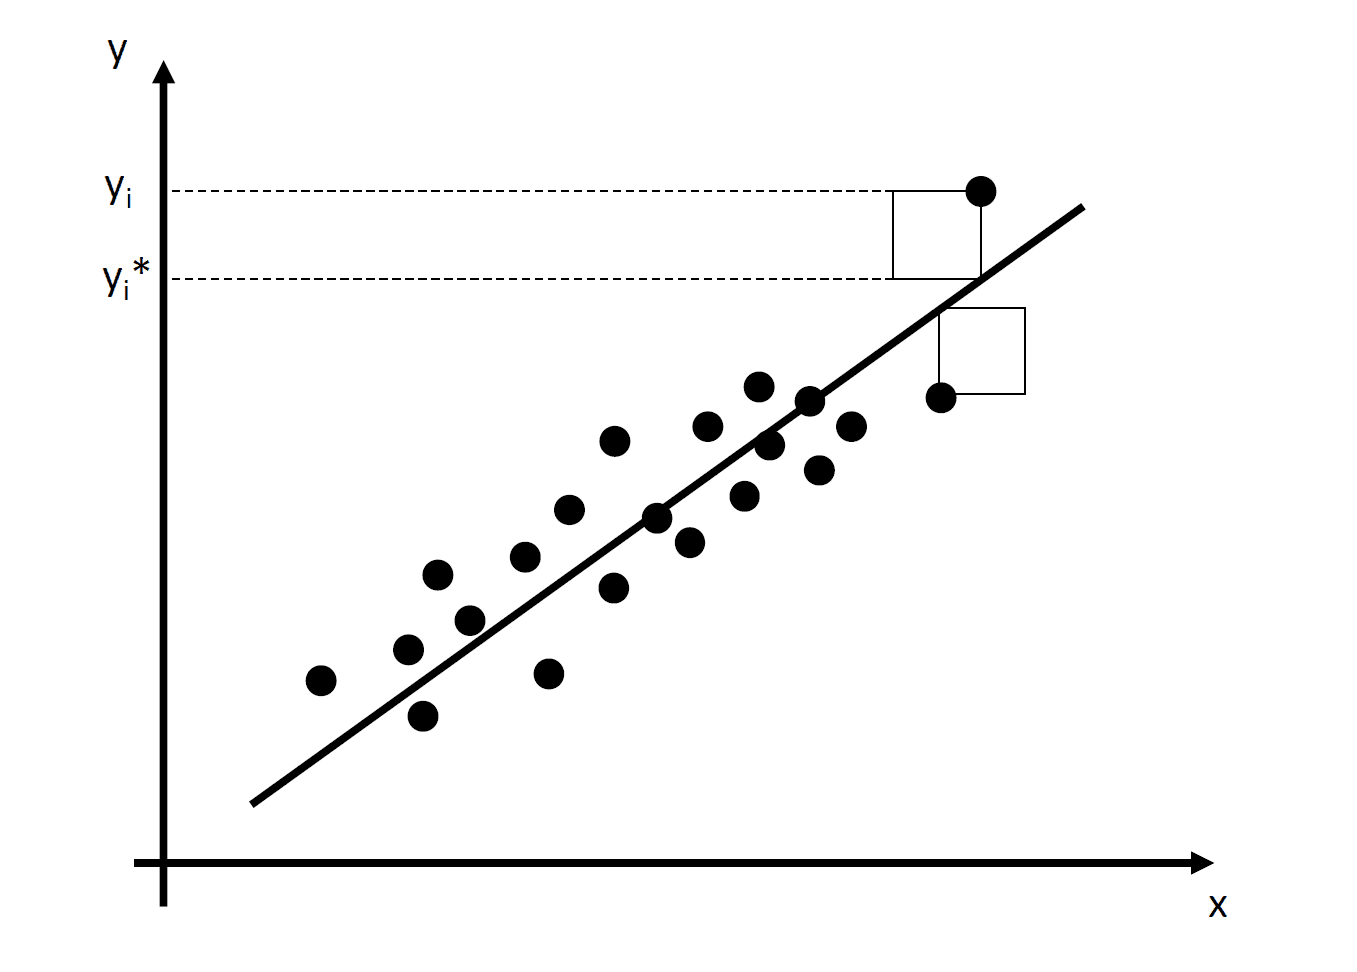
\includegraphics[width=0.5\textwidth,height=\textheight]{fig/regression_ols.png}
\caption{\label{fig:regressionols} The fitted line and the residuals}
\end{figure}

Thus, we minimize the squared residuals by choosing the estimated coefficients \(\hat{\beta_{0}}\) and \(\hat{\beta_{1}}\)
\begin{align*}
\min_{\hat{\beta_{0}}, \hat{\beta_{1}}}\sum_{i=1} \epsilon_i^2 &= \sum_{i=1}    \left[y_i - \underbrace{(\hat{\beta_{0}} + \hat{\beta_{1}} x_i)}_{\text{predicted values}\equiv y_i^*}\right]^2\\
\Leftrightarrow  &=  \sum_{i=1} (y_i - \hat{\beta_{0}} - \hat{\beta_{1}} x_i)^2
\end{align*}
Minimizing the function requires to calculate the first order conditions with respect to alpha and beta and set them zero:
\begin{align*}
\frac{\partial \sum_{i=1} \epsilon_i^2}{\partial \beta_{0}}=2 \sum_{i=1}    (y_i - \hat{\beta_{0}} - \hat{\beta_{1}} x_i)=0\\
\frac{\partial \sum_{i=1} \epsilon_i^2}{\partial \beta_{1}}=2 \sum_{i=1}    (y_i - \hat{\beta_{0}} - \hat{\beta_{1}} x_i)x_i=0
\end{align*}
This is just a linear system of two equations with two unknowns \(\beta_{0}\) and \(\beta_{1}\), which we can mathematically solve for \(\beta_0\):
\begin{align*}
    &\sum_{i=1} (y_i - \hat{\beta_{0}} - \hat{\beta_{1}} x_i)=0\\
    \Leftrightarrow \hat{\beta_{0}}&=\frac{1}{n}\sum_{i=1}  (y_i  - \hat{\beta_{1}} x_i)\\
    \Leftrightarrow \hat{\beta_{0}}&=\bar{y}-\hat{\beta_{1}}\bar{x}
\end{align*}
and for \(\beta_{1}\):
\begin{align*}
    &\sum_{i=1} (y_i - \hat{\beta_{0}} - \hat{\beta_{1}} x_i)x_i=0\\
    \Leftrightarrow & \sum_{i=1}    y_i x_i- \underbrace{\hat{\beta_{0}}}_{\bar{y}-\hat{\beta_{1}}\bar{x}}x_i - \hat{\beta_{1}} x_i^2=0\\
    \Leftrightarrow & \sum_{i=1}    y_i x_i- (\bar{y}-\hat{\beta_{1}}\bar{x})x_i - \hat{\beta_{1}} x_i^2=0\\    
    \Leftrightarrow & \sum_{i=1}    y_i x_i- \bar{y}x_i-\hat{\beta_{1}}\bar{x}x_i - \hat{\beta_{1}} x_i^2=0\\   
    \Leftrightarrow & \sum_{i=1}    (y_i - \bar{y}-\hat{\beta_{1}}\bar{x} - \hat{\beta_{1}} x_i)x_i=0\\ 
%   \Leftrightarrow & \sum_{i=1}    (y_i - \bar{y})-\beta_{1}\bar{x} - \hat{\beta_{1}} x_i=0\\
    \Leftrightarrow & \sum_{i=1} (y_i - \bar{y}) x_i -\hat{\beta_{1}}(\bar{x} -  x_i)x_i =0\\
    \Leftrightarrow & \sum_{i=1}    (y_i - \bar{y}) x_i  =  \hat{\beta_{1}} \sum_{i=1} (\bar{x} -  x_i) x_i \\
%   \Leftrightarrow & \beta_{1} =\frac{\sum_{i=1}(y_i - \bar{y})x_i }{ \sum_{i=1} (\bar{x} -  x_i)x_i }\\
    \Leftrightarrow & \hat{\beta_{1}} =\frac{\sum_{i=1}(y_i - \bar{y})x_i }{ \sum_{i=1} (\bar{x} -  x_i)x_i }\\
        \Leftrightarrow & \hat{\beta_{1}} =\frac{\sum_{i=1}(y_i -\bar{y})(x_i-\bar{x})}{\sum_{i=1} (\bar{x} -  x_i)^2 }\\
    \Leftrightarrow & \hat{\beta_{1}} ={\frac {\sigma_{x,y}}{\sigma^2_{x}}}
\end{align*}
The estimated regression coefficient \(\hat{\beta_{1}}\) equals the covariance between \(y\) and \(x\) divided by the variance of \(x\).

The formulas presented above may not be very intuitive at first glance. The online version of the book \citet{Hanck2020Introduction} offers a nice interactive application in the box \href{https://www.econometrics-with-r.org/4-2-estimating-the-coefficients-of-the-linear-regression-model.html}{The OLS Estimator, Predicted Values, and Residuals} that helps to understand the mechanics of OLS. You can add observations by clicking into the coordinate system where the data are represented by points. Once two or more observations are available, the application computes a regression line using OLS and some statistics which are displayed in the right panel. The results are updated as you add further observations to the left panel. A double-click resets the application, i.e., all data are removed.

\hypertarget{the-least-squares-assumptions}{%
\subsubsection{The least squares assumptions}\label{the-least-squares-assumptions}}

OLS performs well under a quite broad variety of different circumstances. However, there are some assumptions which need to be satisfied in order to ensure that the estimates are normally distributed in large samples.

The Least Squares Assumptions should fulfill the following assumptions:
\[Y_i = \beta_0 + \beta_1 X_i + \epsilon_i \text{, } i = 1,\dots,n\]
- The error term \(\epsilon_i\) has conditional mean zero given \(X_i: E(u_i|X_i)=0\).
- \((X_i,Y_i), i=1,\dots,n\) are independent and identically distributed (i.i.d.) draws from their joint distribution.
- Large outliers are unlikely: \(X_i\) and \(Y_i\) have nonzero finite fourth moments. That means, assumption 3 requires that \(X\) and \(Y\) have a finite kurtosis.

\hypertarget{measures-of-fit}{%
\subsubsection{Measures of fit}\label{measures-of-fit}}

After fitting a linear regression model, a natural question is how well the model describes the data. Visually, this amounts to assessing whether the observations are tightly clustered around the regression line. Both the coefficient of determination and the standard error of the regression measure how well the OLS Regression line fits the data.

\(R^2\) is the fraction of the sample variance of \(Y_i\) that is explained by \(X_i\). Mathematically, the \(R^2\) can be written as the ratio of the explained sum of squares to the total sum of squares. The explained sum of squares (ESS) is the sum of squared deviations of the predicted values \(\hat{Y_i}\), from the average of the \(Y_i\). The total sum of squares (TSS) is the sum of squared deviations of the \(Y_i\) from their average. Thus we have
\begin{align}
ESS & =  \sum_{i = 1}^n \left( \hat{Y_i} - \overline{Y} \right)^2,   \\
TSS & =  \sum_{i = 1}^n \left( Y_i - \overline{Y} \right)^2,   \\
R^2 & = \frac{ESS}{TSS}.
\end{align}
Since \(TSS = ESS + SSR\) we can also write
\[R^2 = 1- \frac{\textcolor{blue}{SSR}}{\textcolor{red}{TSS}}\]
with \(SSR= \sum_{i = 1}^n \epsilon^2\).

\begin{figure}
\centering
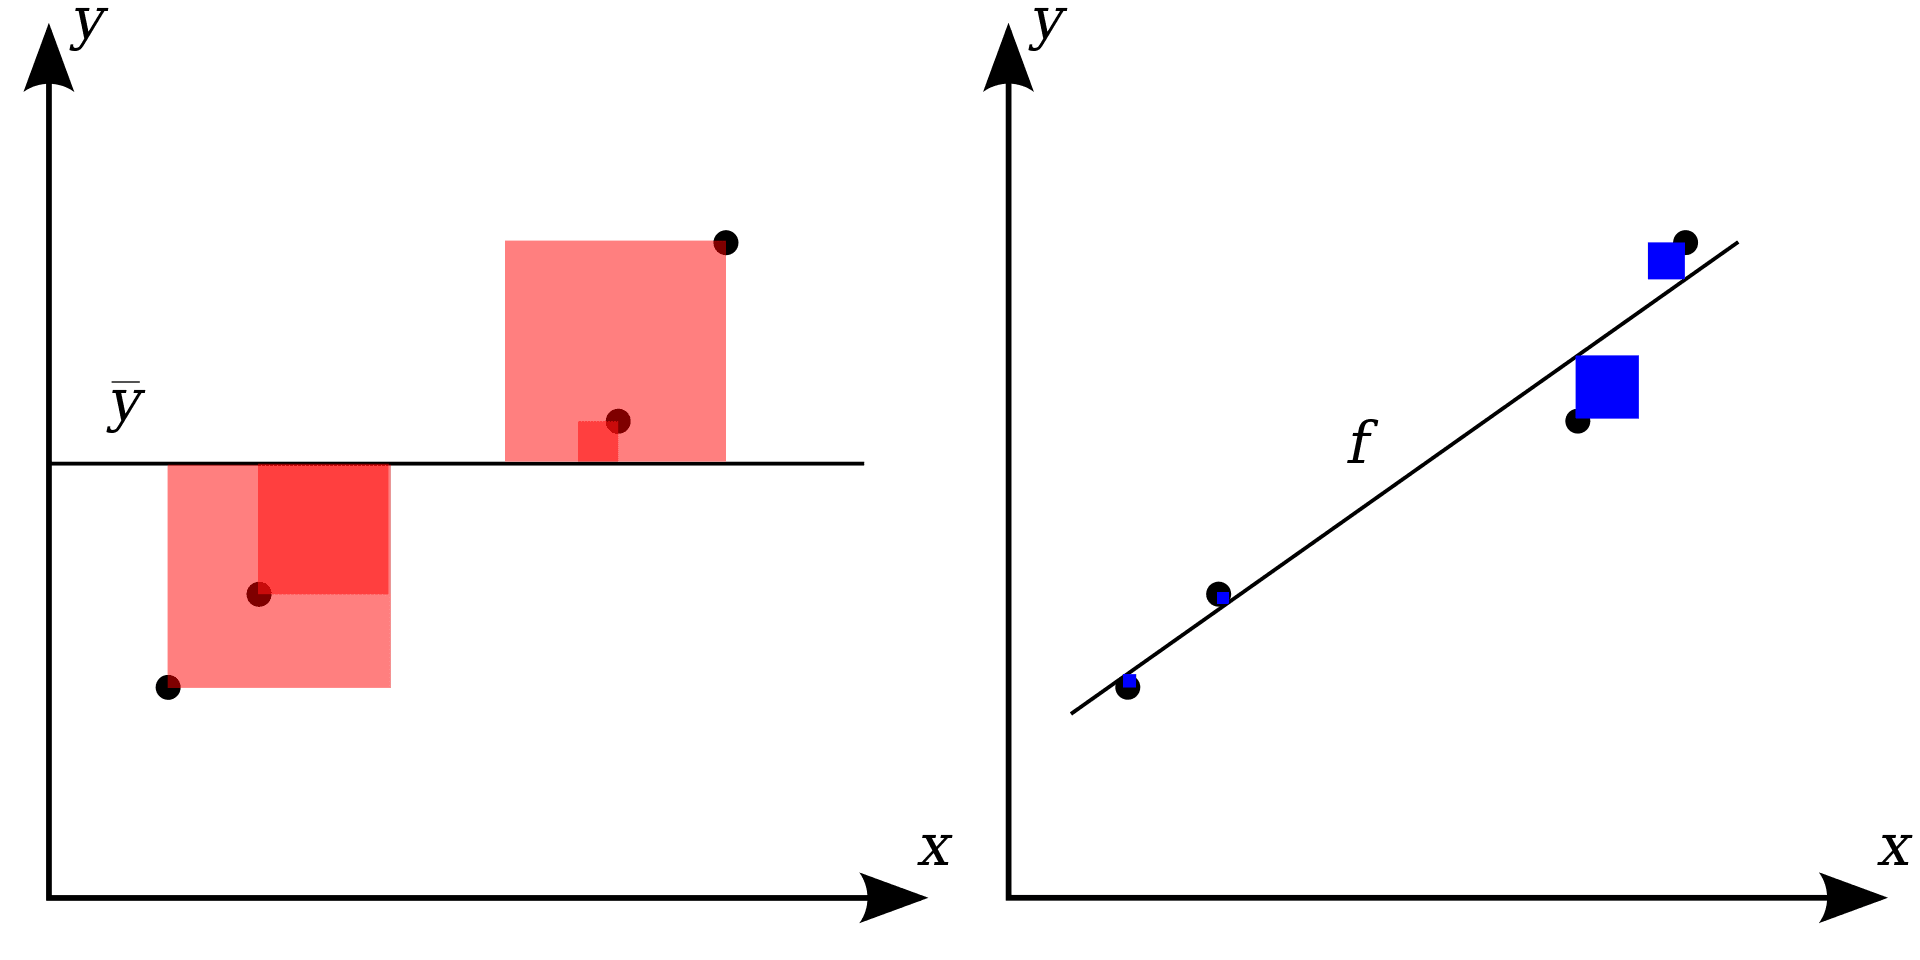
\includegraphics[width=0.75\textwidth,height=\textheight]{fig/fitR.png}
\caption{\label{fig:fitR} Total sum of squares and sum of squared residuals}
\end{figure}

\(R^2\) lies between 0 and 1. It is easy to see that a perfect fit, i.e., no errors made when fitting the regression line, implies \(R2=1\) since then we have \(SSR=0\). On the contrary, if our estimated regression line does not explain any variation in the \(Y_i\), we have \(ESS=0\) and consequently \(R^2=0\). Figure \ref{fig:fitR} show the relationship of TTS and SSR.

\hypertarget{multiple-linear-regression}{%
\subsection{Multiple linear regression}\label{multiple-linear-regression}}

Having understood the simple linear regression model, it is important to broaden our scope beyond the relationship between just two variables: the dependent variable and a single regressor. Our goal is to causally interpret the measured association of two variables, which requires certain conditions as explained in section \ref{identification}.

To illustrate this concept, let's revisit the phenomenon known as Simpson's paradox. Simpson's paradox occurs when the overall association between two categorical variables differs from the association observed when we consider the influence of one or more other variables, known as controlling variables. This paradox holds three key reasons for its significance.

Firstly, it challenges the assumption that statistical relationships are fixed and unchanging. In reality, the relationship between two variables can vary, either increasing, decreasing, or even changing direction depending on the set of variables being controlled.

Secondly, Simpson's paradox is not an isolated phenomenon of interest solely to statisticians. It belongs to a larger class of association paradoxes, indicating that similar situations can arise in various contexts.

Lastly, Simpson's paradox serves as a reminder to researchers about the potential pitfalls of making causal inferences, especially in nonexperimental studies. Uncontrolled or unobserved variables may exist that can eliminate or reverse the observed association between two variables.

Thus, it is important to consider confounding variables to ensure valid and reliable causal interpretations in research, particularly in nonexperimental settings.

\begin{figure}
\centering
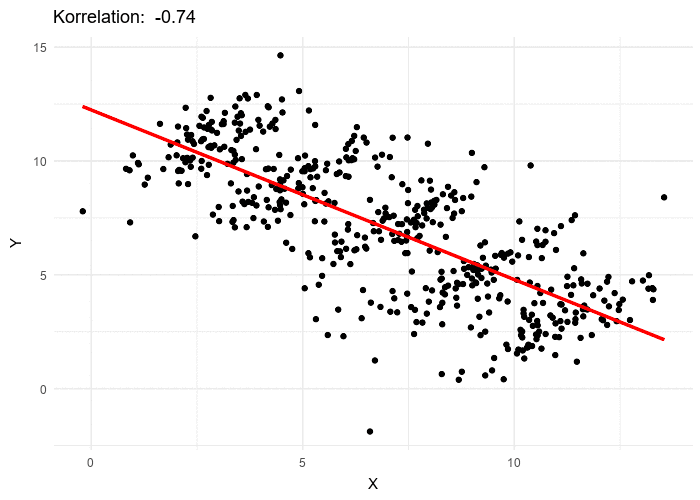
\includegraphics[width=0.75\textwidth,height=\textheight]{fig/foo-13.png}
\caption{\label{fig:foo13} Simpsons paradox and the power of controlling variables (1)}
\end{figure}

\begin{figure}
\centering
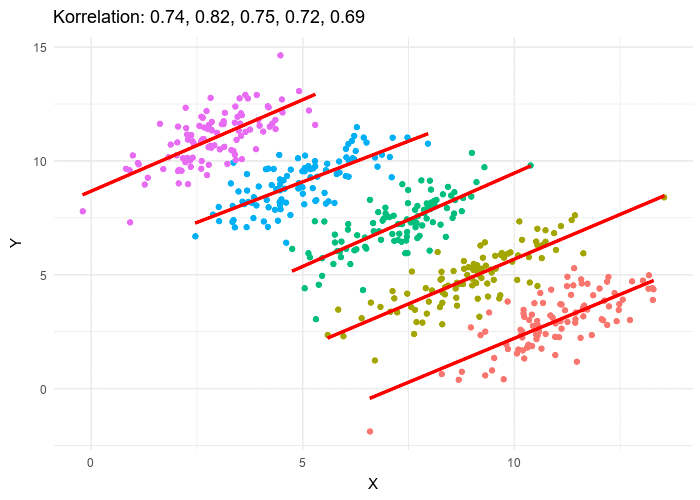
\includegraphics[width=0.75\textwidth,height=\textheight]{fig/foo-32.png}
\caption{\label{fig:foo32} Simpsons paradox and the power of controlling variables (1)}
\end{figure}

The multiple regression model can be expressed as
\[
Y_i = \beta_0 + \beta_1 X_{1i} + \beta_2 X_{2i} + \beta_3 X_{3i} + \dots + \beta_k X_{ki} + u_i, \ i=1,\dots,n.
\]

How can we estimate the coefficients of the multiple regression model? As in the simple model, we seek to minimize the sum of squared mistakes by choosing estimated
coefficients \(\beta_0,\beta_1,\dots,\beta_k\) such that
\[\sum_{i=1}^n (Y_i - b_0 - b_1 X_{1i} - b_2 X_{2i} - \dots -  b_k X_{ki})^2 \]

This demands matrix notation. This goes beyond the scope of this introduction.

\hypertarget{gauss-markov-and-the-best-linear-unbiased-estimator}{%
\subsubsection{Gauss-Markov and the best linear unbiased estimator}\label{gauss-markov-and-the-best-linear-unbiased-estimator}}

The Gauss-Markov assumptions, also known as the classical linear regression assumptions, are a set of assumptions that underlie the ordinary least squares (OLS) method for estimating the parameters in a linear regression model. These assumptions ensure that the OLS estimators are unbiased, efficient, and have desirable statistical properties.

The Gauss-Markov assumptions are as follows:

\begin{enumerate}
\def\labelenumi{\arabic{enumi}.}
\item
  Linearity: The relationship between the dependent variable and the independent variables is linear in the population model. This means that the true relationship between the variables can be represented by a linear equation.
\item
  Independence: The errors (residuals) in the regression model are independent of each other. This assumption ensures that the errors for one observation do not depend on or influence the errors for other observations.
\item
  Strict exogeneity: The errors have a mean of zero conditional on all the independent variables. In other words, the expected value of the errors is not systematically related to any of the independent variables.
\item
  No perfect multicollinearity: The independent variables are not perfectly correlated with each other. Perfect multicollinearity occurs when one independent variable is a perfect linear combination of other independent variables, leading to problems in estimating the regression coefficients.
\item
  Homoscedasticity: The errors have constant variance (homoscedasticity) across all levels of the independent variables. This assumption implies that the spread or dispersion of the errors is the same for all values of the independent variables.
\item
  No endogeneity: The errors are not correlated with any of the independent variables. Endogeneity occurs when there is a correlation between the errors and one or more of the independent variables, leading to biased and inefficient estimators.
\item
  No autocorrelation: The errors are not correlated with each other, meaning that there is no systematic pattern or relationship between the errors for different observations.
\end{enumerate}

These assumptions collectively ensure that the OLS estimators are unbiased, efficient, and have minimum variance among all linear unbiased estimators. Violations of these assumptions can lead to biased and inefficient estimators, invalid hypothesis tests, and unreliable predictions. Therefore, it is important to check these assumptions when using the OLS method and consider alternative estimation techniques if the assumptions are violated.

\hypertarget{confounding-and-control-variables}{%
\subsubsection{Confounding and control variables}\label{confounding-and-control-variables}}

A confounding variable is a factor that was not accounted for or controlled in a study but has the potential to influence the results. In other words, the true effects of the treatment or intervention can be obscured or muddled by the presence of this variable.

For instance, let's consider a scenario where two groups of individuals are observed: one group took vitamin C daily, while the other group did not. Over the course of a year, the number of colds experienced by each group is recorded. It might be observed that the group taking vitamin C had fewer colds compared to the group that did not. However, it would be incorrect to conclude that vitamin C directly reduces the occurrence of colds. Since this study is observational and not a true experiment, numerous confounding variables are at play. One potential confounding variable could be the individuals' level of health consciousness. Those who take vitamins regularly might also engage in other health-conscious behaviors, such as frequent handwashing, which could independently contribute to a lower risk of catching colds.

To address confounding variables, researchers employ control measures. The idea is to create conditions where confounding variables are minimized or eliminated. In the aforementioned example, researchers could pair individuals who have similar levels of health consciousness and randomly assign one person from each pair to take vitamin C daily (while the other person receives a placebo). Any differences observed in the number of colds between the groups would be more likely attributable to the vitamin C, compared to the original observational study. Well-designed experiments are crucial as they actively control for potential confounding variables.

Consider another scenario where a researcher claims that eating seaweed prolongs life. However, upon reading interviews with the study subjects, it becomes apparent that they were all over 100 years old, followed a very healthy diet, slept an average of 8 hours per day, drank ample water, and engaged in regular exercise. In this case, it is not possible to determine whether longevity was specifically caused by seaweed consumption due to the presence of numerous confounding variables. The healthy diet, sufficient sleep, hydration, and exercise could all independently contribute to longer life. These variables act as confounding factors.

A common error in research studies is to fail to control for confounding variables, leaving the results open to scrutiny. The best way to head off confounding variables is to do a well-designed experiment in a controlled setting. Observational studies are great for surveys and polls, but not for showing cause-and-effect relationships, because they don't control for confounding variables.

\textbf{Control variables} are usually variables that you are not particularly interested in, but that are related to the dependent variable. You want to remove their effects from the equation. A control variable enters a regression in the same way as an independent variable -- the method is the same.

Nick Huntington-Klein offers \href{https://www.nickchk.com/causalgraphs.html}{Causal Inference Animated Plots} on his homepage. Read this page and consider the animated graphs.

\hypertarget{omitted-variable-bias-and-ceteris-paribus}{%
\subsubsection{Omitted variable bias and ceteris paribus}\label{omitted-variable-bias-and-ceteris-paribus}}

From the Gauss-Markov theorem we know that if the OLS assumptions are fullfiled, the OLS estimator is (in the sense of smallest variance) the best linear conditionally unbiased estimator (BLUE).
However, OLS estimates can suffer from omitted variable bias when any regressor, X, is correlated with any omitted variable that matters for variable Y.

For omitted variable bias to occur, two conditions must be fulfilled:

\begin{enumerate}
\def\labelenumi{\arabic{enumi}.}
\tightlist
\item
  X is correlated with the omitted variable.
\item
  The omitted variable is a determinant of the dependent variable Y.
\end{enumerate}

In regression analysis, ``ceteris paribus'' is a Latin phrase that translates to ``all other things being equal'' or ``holding everything else constant.'' It is a concept used to examine the relationship between two variables while assuming that all other factors or variables remain unchanged.

When we say \emph{ceteris paribus} in the context of regression analysis, we are isolating the effect of a specific independent variable on the dependent variable while assuming that the values of the other independent variables remain constant. By holding other variables constant, we can focus on understanding the direct relationship between the variables of interest.

For example, consider a regression analysis that examines the relationship between income (dependent variable) and education level (independent variable) while controlling for age, gender, and work experience. By stating \emph{ceteris paribus}, we are assuming that age, gender, and work experience remain constant, and we are solely interested in understanding the impact of education level on income.

\begin{exercise}
\protect\hypertarget{exr:lookatoutput}{}\label{exr:lookatoutput}

Look at the Output

\begin{figure}
\centering
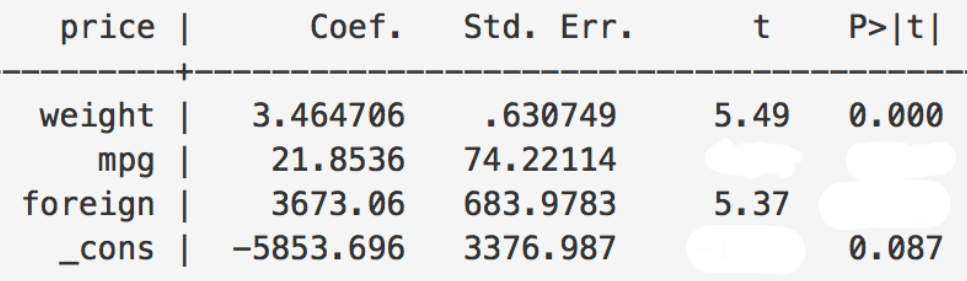
\includegraphics[width=0.85\textwidth,height=\textheight]{fig/reg_stata2.png}
\caption{\label{fig:regstata2} Regression output}
\end{figure}

Above you see an excerpt of a regression output taken from a statistical program. Some t-values and p-values are missing.

\begin{enumerate}
\def\labelenumi{\alph{enumi})}
\tightlist
\item
  Calculate the t-value of the coefficient \texttt{mpg}. Is the coefficient at a level of \(\alpha=0.05\) statistically significant?\\
\item
  Is the coefficient foreign at a level of \(\alpha=0.05\) statistically significant?\\
\item
  Is the constant at a level of \(\alpha=0.05\) statistically significant?
\end{enumerate}

\end{exercise}

\begin{exercise}
\protect\hypertarget{exr:exrstataoutput}{}\label{exr:exrstataoutput}Look at Stata Output

Below you find two regression outputs from Stata. Try to interpret the p-values and the confidence intervals. How are the t-values calculated. Can you use the \emph{magic number} 1.96 to say if a corresponding estimated coefficient is statistically significant, or not? Which estimated model is \emph{better}?

\begin{figure}
\centering
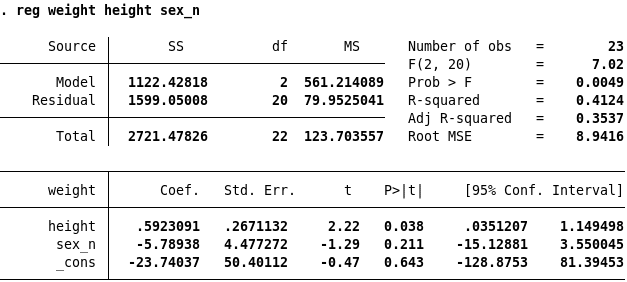
\includegraphics[width=0.85\textwidth,height=\textheight]{fig/reg_stata_class2.png}
\caption{\label{fig:regstata3} Stata regression output (1)}
\end{figure}

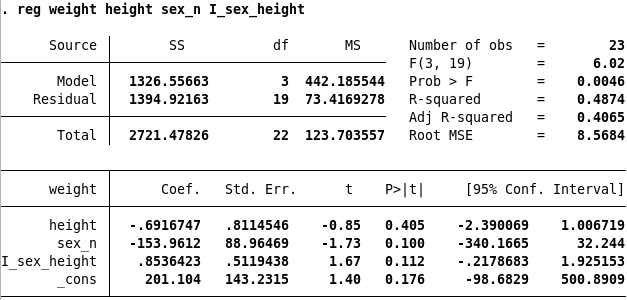
\includegraphics[width=0.85\textwidth,height=\textheight]{fig/reg_stata_class.png}
\end{exercise}

\begin{exercise}
\protect\hypertarget{exr:explainweight}{}\label{exr:explainweight}Explain the weight

Download the file \href{https://github.com/hubchev/courses/blob/main/pdfs/exe_calories.pdf}{exe\_calories.pdf} from GitHub and answer the questions therein.

Solutions are provided \href{https://raw.githubusercontent.com/hubchev/courses/main/scr/regress_lecture.R}{here}.
\end{exercise}

\hypertarget{hands-on-experiments}{%
\chapter{Hands on experiments}\label{hands-on-experiments}}

\hypertarget{natural-experiments}{%
\section{Natural experiments}\label{natural-experiments}}

In social science, a \emph{natural experiment} is a research design that exploits naturally occurring circumstances or events to study the effects of an intervention or treatment. In these experiments, the treatment is not manipulated by the researcher, but is instead determined by exogenous, or external, factors. \emph{Exogenous variations} refer to changes in the independent variable that are not caused by the researcher's actions but instead occur naturally or through some external factor. These variations are often unpredictable and occur without the intervention of the researcher, making them an ideal source of variation to study the causal effects of a treatment or intervention.
One example of a natural experiment is the partition of Germany after World War II, which created two economies that were initially similar but experienced vastly different economic and institutional environments. Another example is the introduction of a new policy or technology in one state or country but not in another, allowing for a comparison of outcomes before and after the treatment.
A natural experiment might involve comparing the outcomes of two groups of people who were exposed to different levels of air pollution due to a policy change or a natural disaster. In this case, the variation in air pollution levels is exogenous, since it is not controlled by the researcher but rather determined by external factors.

By leveraging these exogenous variations, researchers can better estimate the causal effects of an intervention or treatment, and provide evidence for policy-makers to make more informed decisions. In the following, we will get known to some studies that are based on natural experiments.

\hypertarget{empirical-evidence-bombing}{%
\section{Empirical evidence: Bombing}\label{empirical-evidence-bombing}}

In their article ``Bones, Bombs, and Break Points: The Geography of Economic Activity,'' \citet{Davis2002Bones} explore another natural experiment that has shaped the economic geography of the world: the natural endowment of different regions with physical and institutional factors that affect their productivity and attractiveness to economic activity. Using a spatial econometric model, they test the relative importance of three such factors: climate, natural resources, and political borders. They find that political borders, such as the ones that emerged from colonialism or ethnic conflict, have the strongest effect on economic activity, even after controlling for other factors. This has important implications for policy, as it suggests that changing the institutional environment of a region can have a significant impact on its economic performance.

Overall, Davis and Weinstein's article demonstrates the power of natural experiments to shed light on important economic questions and inform policy debates. By examining the historical and geographical factors that have shaped economic activity around the world, they offer valuable insights into the mechanisms that drive economic growth and inequality.

\begin{figure}
\centering
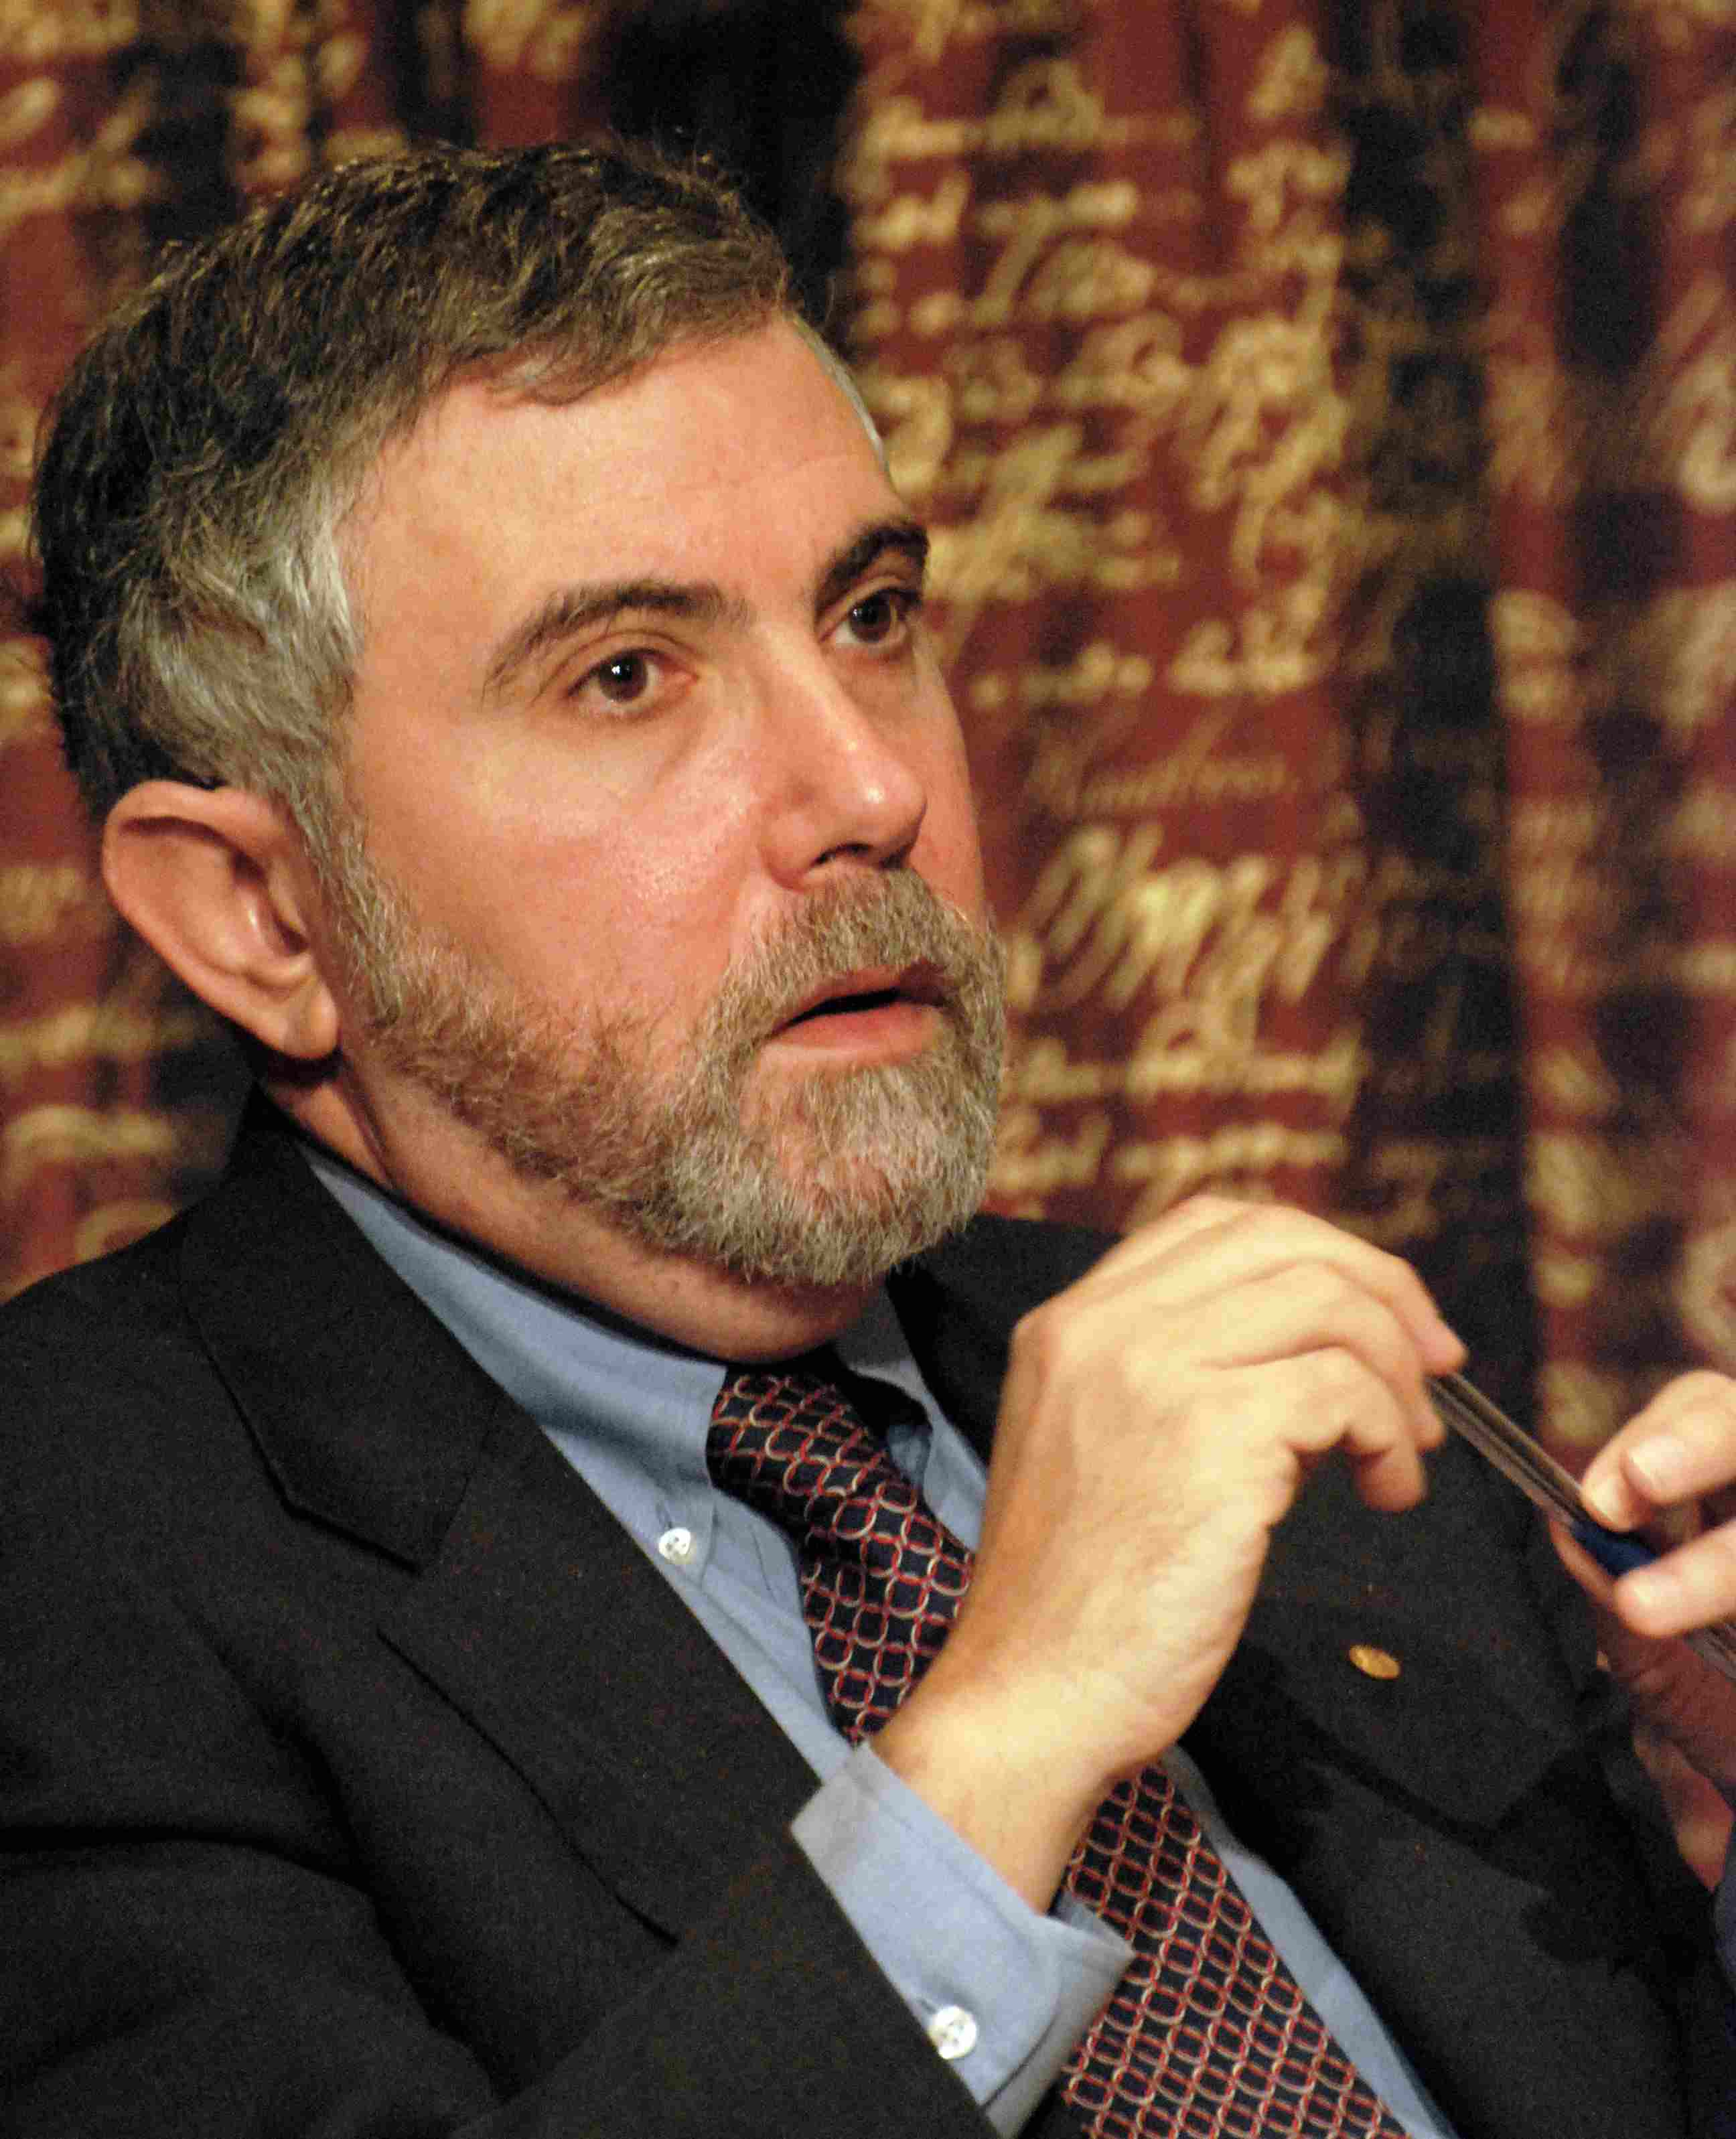
\includegraphics[width=0.3\textwidth,height=\textheight]{fig/krugman.jpeg}
\caption[\label{fig:krugman} Paul Krugman *1953]{\label{fig:krugman} Paul Krugman *1953\footnotemark{}}
\end{figure}
\footnotetext{Picture is taken from \url{https://commons.wikimedia.org/wiki/File:Paul_Krugman-press_conference_Dec_07th,_2008-8.jpg}}

Before you read this article, let me explain that the theory which this article elaborates and tests goes back to the 2008 nobel-prize winner Paul Krugman (*1953) who founded the so-called \emph{New Economic Geography} (NEG).
Here is an excerpt of how the Royal Swedish Academy of Sciences summarizes Krugman's contribution to the field (RSA2008Prize, 3):

\begin{quote}
Economic geography deals not only with what goods are produced where, but also with the distribution of capital and labor over countries and regions. The approach Krugman used in his foreign trade theory -- the assumption of economies of scale in production and a preference for diversity in consumption -- was also found to be appropriate for analyzing geographical issues. This allowed Krugman to integrate two disparate fields in a cohesive model.
\end{quote}

\begin{quote}
The embryo of the theory which would come to be called the ``new economic geography'\,' had already appeared in Krugman's 1979 article. In the final pages, he asks what would happen if foreign trade became impossible, for instance due to excessively high transport costs or other obstacles. His line of reasoning is as follows. If two countries are exactly alike, then welfare will be the same in both countries. But if the countries are alike in all respects except that one of them has a slightly larger population than the other, then the real wages of labor will be somewhat higher in the country with more inhabitants. The reason is that firms in the more highly populated country can make better use of economies of scale, which implies lower prices to consumers and/or greater diversity in the supply of goods. This, in turn, enhances the welfare of consumers. As a result, labor, i.e., consumers, will tend to move to the country with more inhabitants, thereby increasing its population. Real wages and the supply of goods will then continue to increase even more in that country, thereby giving rise to further migration, and so on.
\end{quote}

\begin{quote}
Twelve years would pass, however, before Krugman reconsidered these ideas. In an article published in 1991, he developed these concepts into a comprehensive theory of location of labor and firms. Here, he assumes that although trade is possible, it is obstructed due to transport costs. Otherwise, labor is free to move to the country or region which can offer the highest welfare, in terms of real wages and diversity of goods. Firms' location decisions imply a trade-off between utilizing economies of scale and saving on transport costs.
\end{quote}

\begin{quote}
\textbf{Concentration or Decentralization?}
\end{quote}

\begin{quote}
The above considerations evolved into the so-called core-periphery model, which shows that the relation between economies of scale and transport costs can result in either concentration or decentralization of communities. Under certain conditions, the forces which contribute to concentration will dominate. Regional imbalances arise and most of the population will be concentrated in a high-technology core, whereas a small minority will inhabit the periphery and live off agriculture. Such a mechanism could underlie the explosive urbanization witnessed today throughout the world, with rapidly growing megacities surrounded by increasingly depopulated rural areas. This is not necessarily the only possibility, however. Under different conditions, the forces which give rise to decentralization will dominate. This promotes somewhat more balanced development. Krugman's model can be used to account for the mechanisms at work in both directions. For example, his model indicates that declining transport costs easily generate concentration and urbanization -- which seems particularly noteworthy since transport costs have exhibited a declining trend throughout the twentieth century.
\end{quote}

Numerous research papers inspired by Krugman's New Economic Geography (NEG) focus on the origins and implications of the so-called first and second nature effects. These effects are used to explain the uneven distribution of economic activity both across countries and within regions of a country. Two primary explanations have been investigated: (1) \emph{Fundamentals}, which refer to differences in the fundamental productivity of locations, and (2) \emph{Agglomeration forces}, which are related to the proximity of economic agents that boost productivity and make a location more attractive.

These two mechanisms are obviously not exclusive and can both operate simultaneously. The key empirical question is to what extent observed patterns of economic activity are explained by these two mechanisms. Understanding whether fundamentals or agglomeration forces are responsible for the pattern of economic activity has significant implications for the persistence of spatial equilibria and policy making.

For instance, suppose only agglomeration forces are at play. In that case, the location of economic activity is relatively arbitrary, and a particular location is attractive mainly because other workers are choosing to locate there. This phenomenon is similar to selecting a nightclub: club A is crowded and everybody wants to be there only because it was the club had attracted the first person that night.

In contrast, if only fundamentals are in operation, the distribution of activity is determined by the distribution of these underlying factors. When agglomeration forces dominate fundamentals, the spatial distribution of activity becomes a matter of political interest. For example, regional policies can aim to move the distribution of economic activity between different equilibria. Using a temporary subsidy, regions can try to attract a `critical mass' of economic activity. Once established, this critical mass will make the location more attractive, even when the subsidy has ended.

This approach is similar to nightclub policies, such as offering free entry or other discounts to the first people who are searching for a club. These incentives are an attempt to attract a critical mass of party-goers, making the nightclub more attractive and increasing the likelihood that other party-goers will choose the same club later.

\begin{exercise}
\protect\hypertarget{exr:bombs}{}\label{exr:bombs}

The impact of nuclear bombs on agglomerations

\textbf{Background:} The bombing of Japan during the Second World War devastated 66 cities that were targeted, leading to the destruction of approximately half of their housing stock and the deaths of around 300,000 Japanese. Although Hiroshima and Nagasaki are more well-known due to the nuclear bombs that were dropped on them, the majority of cities in the sample suffered little to no destruction, including several large cities. Despite the scale of the bombing, it was clearly a temporary shock that did not change the fundamental attractiveness of locations. However, the nuclear radiation in Hiroshima and Nagasaki could be considered an exception.

\textbf{Data:} The data set used in the paper consists of information on 303 Japanese cities with a population exceeding 30,000 in 1925. Population figures are recorded every five years, with the exception of the 1945 census, which took place in 1947. One way to gauge the intensity of the shocks experienced by the cities is by looking at the number of dead or missing residents.

\begin{enumerate}
\def\labelenumi{\alph{enumi})}
\tightlist
\item
  Read \citet{Davis2002Bones}\footnote{It is available here: \url{https://blogs.cuit.columbia.edu/dew35/files/2016/08/BBB.pdf}} and explain the implications of the following figures:
\end{enumerate}

\begin{figure}
\centering
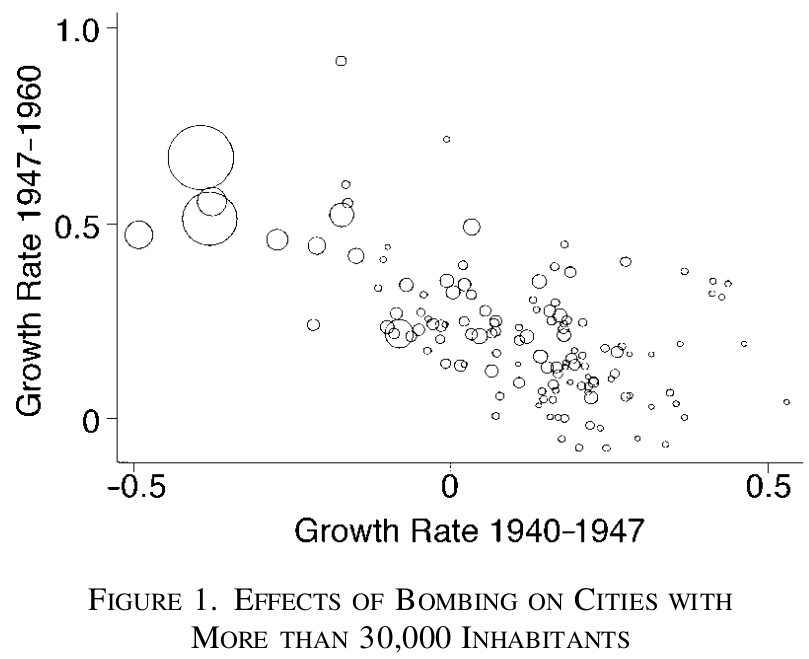
\includegraphics[width=0.8\textwidth,height=\textheight]{fig/fig1weinstein.png}
\caption{\label{fig:fig1weinstein} Figure 1 of \citet{Davis2002Bones}}
\end{figure}

\begin{figure}
\centering
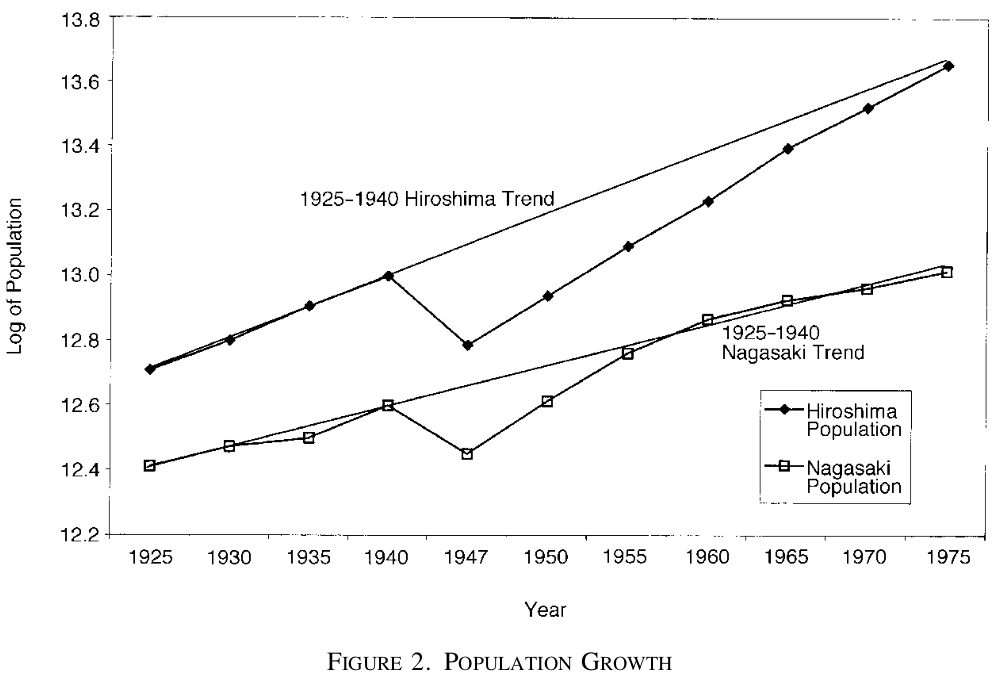
\includegraphics[width=0.8\textwidth,height=\textheight]{fig/fig2weinstein.png}
\caption{\label{fig:fig2weinstein} Figure 2 of \citet{Davis2002Bones}}
\end{figure}

The results of Davis and Weinstein (2002) show a striking persistence of city size even after terrible wartime destruction. This has important implications for attempts to use regional policy to shift economic activity between spatial equilibria. The following quote sums it up well:
\textgreater{} ``An important practical question, then, is whether such spatial catastrophes are theoretical curiosa or a central tendency in the data. Our results provide an unambiguous answer: Even nuclear bombs have little effect on relative city sizes over the course of a couple of decades. The theoretical possibility of spatial catastrophes due to temporary shocks is not a central tendency borne out in the data.'' \citet[p.~1284]{Davis2002Bones}

The use of bombing as a temporary shock, however, can be seen as problematic:
Although bombing causes casualties and destroys housing and social structures, legal property rights and operating licenses are not destroyed. Therefore, rebuilding cities may prove less burdensome than building new settlements from scratch. Moreover, even after a nuclear explosion, functioning infrastructure may still be in place, which could make rebuilding at the old site less costly.

\begin{enumerate}
\def\labelenumi{\alph{enumi})}
\setcounter{enumi}{1}
\tightlist
\item
  Read \citet{Bleakley2012Portage} and discuss how this is confronting the insights from \citet{Davis2002Bones}. It is freely available \href{https://personal.lse.ac.uk/sturmd/brixen/pdf/Bleakley-Lin-QJE-2012.pdf}{here}
\end{enumerate}

\end{exercise}

\begin{exercise}
\protect\hypertarget{exr:natexperiments}{}\label{exr:natexperiments}

Natural experiments in research

\begin{enumerate}
\def\labelenumi{\alph{enumi})}
\tightlist
\item
  Think of other natural experiments that can be scientifically exploited.
\item
  Download \citet{Sieweke2020Natural}. It is freely available here: \url{https://openaccess.city.ac.uk/id/eprint/23363/1/}
\end{enumerate}

\begin{itemize}
\tightlist
\item
  Read section 3.1.
\item
  Study table V.
\end{itemize}

\end{exercise}

\hypertarget{field-experiments-would-you-work-more-if-wages-are-high}{%
\section{Field experiments: Would you work more if wages are high?}\label{field-experiments-would-you-work-more-if-wages-are-high}}

Unlike laboratory experiments, which are conducted in a controlled environment, field experiments are conducted in real-world settings, such as schools, workplaces, and communities. They allow for testing causality by controlling the independent variable while observing the dependent variable in a naturalistic setting. They are a valuable tool for testing the effectiveness of policies and interventions in real-world situations. The level of external validity is usually much higher than alternative methods, meaning that the results can be generalized to other similar contexts beyond the specific setting where the experiment was conducted. In addition, field experiments can help identify unintended consequences of policies or interventions that might not be observable in laboratory experiments or observational studies.

Another advantage of field experiments is that they can be used to test theories in contexts where observational studies may be limited. For example, a theory may predict that a certain policy or intervention will have a specific effect, but it may be difficult to test this theory through observational studies due to confounding variables or selection bias.

However, field experiments can be costly and time-consuming to conduct. Please give \citet{Harrison2004Field} article a quick read, as it explains the nature and advantages of field experiments well.

\begin{exercise}
\protect\hypertarget{exr:fieldexperiments}{}\label{exr:fieldexperiments}

Field experiments in research

\begin{enumerate}
\def\labelenumi{\alph{enumi})}
\tightlist
\item
  Read \citet{Fehr2007Do}. Summarize the results.
\item
  Explain the identification strategy and the experimental design.
\item
  Read \citet{Bandiera2011Field}. Can you think of field studies that organizations could conduct to improve their business?
\end{enumerate}

\end{exercise}

\hypertarget{hands-on-observational-data}{%
\chapter{Hands on observational data}\label{hands-on-observational-data}}

\hypertarget{difference-in-difference}{%
\section{Difference in difference}\label{difference-in-difference}}

\begin{figure}
\centering
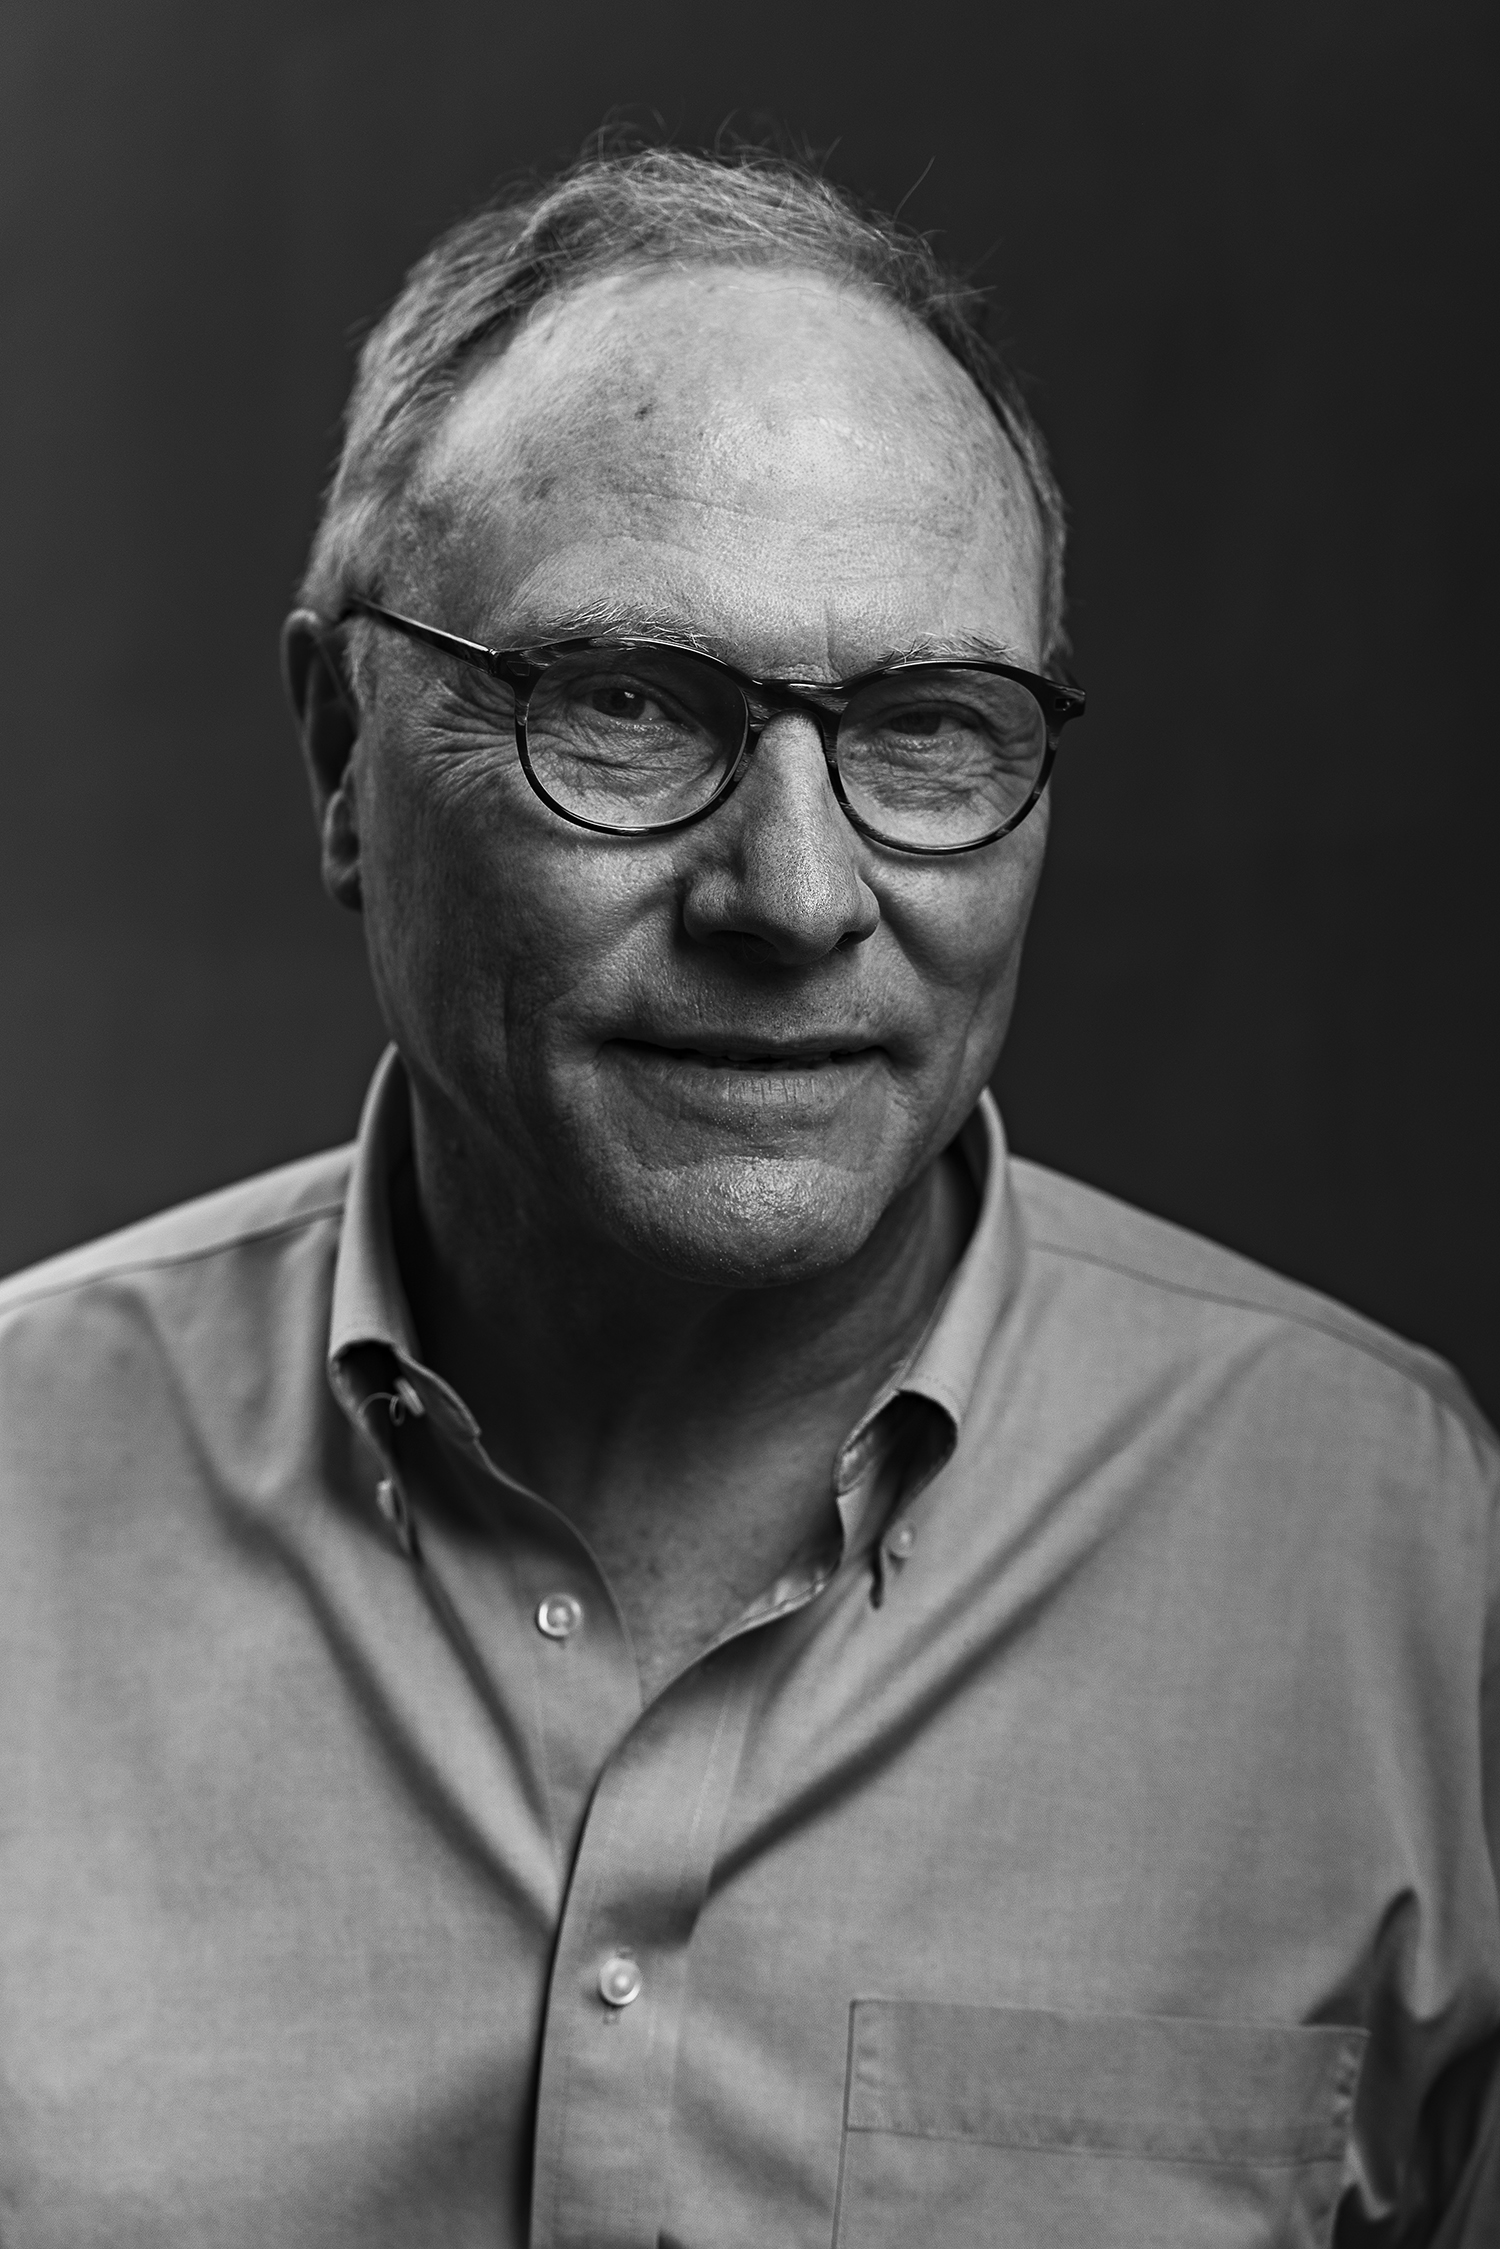
\includegraphics[width=0.25\textwidth,height=\textheight]{fig/dcard1.jpg}
\caption[\label{fig:dcard} David Card (*1956)]{\label{fig:dcard} David Card (*1956)\footnotemark{}}
\end{figure}
\footnotetext{Photo stems from his public homepage \url{https://davidcard.berkeley.edu/}}

David Card is one of the most influential labor economist of the 20th century and Nobel laureate of 2021. He is well-known for his research on the effects of the minimum wage on employment, which challenged the traditional view that increasing the minimum wage leads to a decrease in employment. In his article \emph{Minimum Wages and Employment: A Case Study of the Fast-Food Industry in New Jersey and Pennsylvania} \citep{Card1994Minimum} he and Alan Krueger (1960-2019) used a \emph{natural experiment} to examine the effect of an increase in the minimum wage on employment. In particular, they identified a treatment group (restaurants in New Jersey) and a control group (restaurants in eastern Pennsylvania) to measure the effect of increasing the minimum wage that was increased in New Jersey but not in Pennsylvania. This increase did not lead to a decrease in employment, which contradicted the widely held view that increasing the minimum wage would lead to job loss.
The empirical method that they used is called \emph{difference in difference} and we discuss it in the following section.

The difference in difference (DiD) method allows to estimate the causal effect of a treatment or intervention. In particular, it is popular to study the impact of policy changes and other interventions on a specific outcome of interest.

The basic idea behind the DiD method is to compare the change in an outcome variable between a treatment group and a control group over time. The treatment group is the group that is exposed to the intervention or treatment, while the control group is a group that is not exposed to the intervention. The difference in the change in the outcome variable between the two groups is then used to estimate the causal effect of the intervention.

To use the DiD method, researchers typically collect data on the outcome variable of interest for both the treatment and control groups before and after the intervention. This data is then used to calculate the difference in the change in the outcome variable between the two groups.

For example, if a study aims to examine the effect of a new policy on the employment rate, it should collect data on the employment rate for a group of individuals living in a region where the policy was implemented, and for a group living in a similar region where the policy was not implemented. The study can then compare the change in the employment rate for the two groups, before and after the implementation of the policy. The difference in the change in the employment rate between the two groups can be used to estimate of the causal effect of the policy on employment.

It is important to note that DiD assumes that there are no other factors that could be affecting the outcome variable of interest and that the treatment and control groups are similar in all ways except for the intervention. To control for these assumptions researchers can use statistical techniques such as matching to ensure that treatment and control groups are similar before the intervention.

DiD is useful when we only have observational data and in situations where it is not possible or ethical to randomly assign individuals to a treatment or control group, for example, in the case of policy changes.

\begin{figure}
\centering
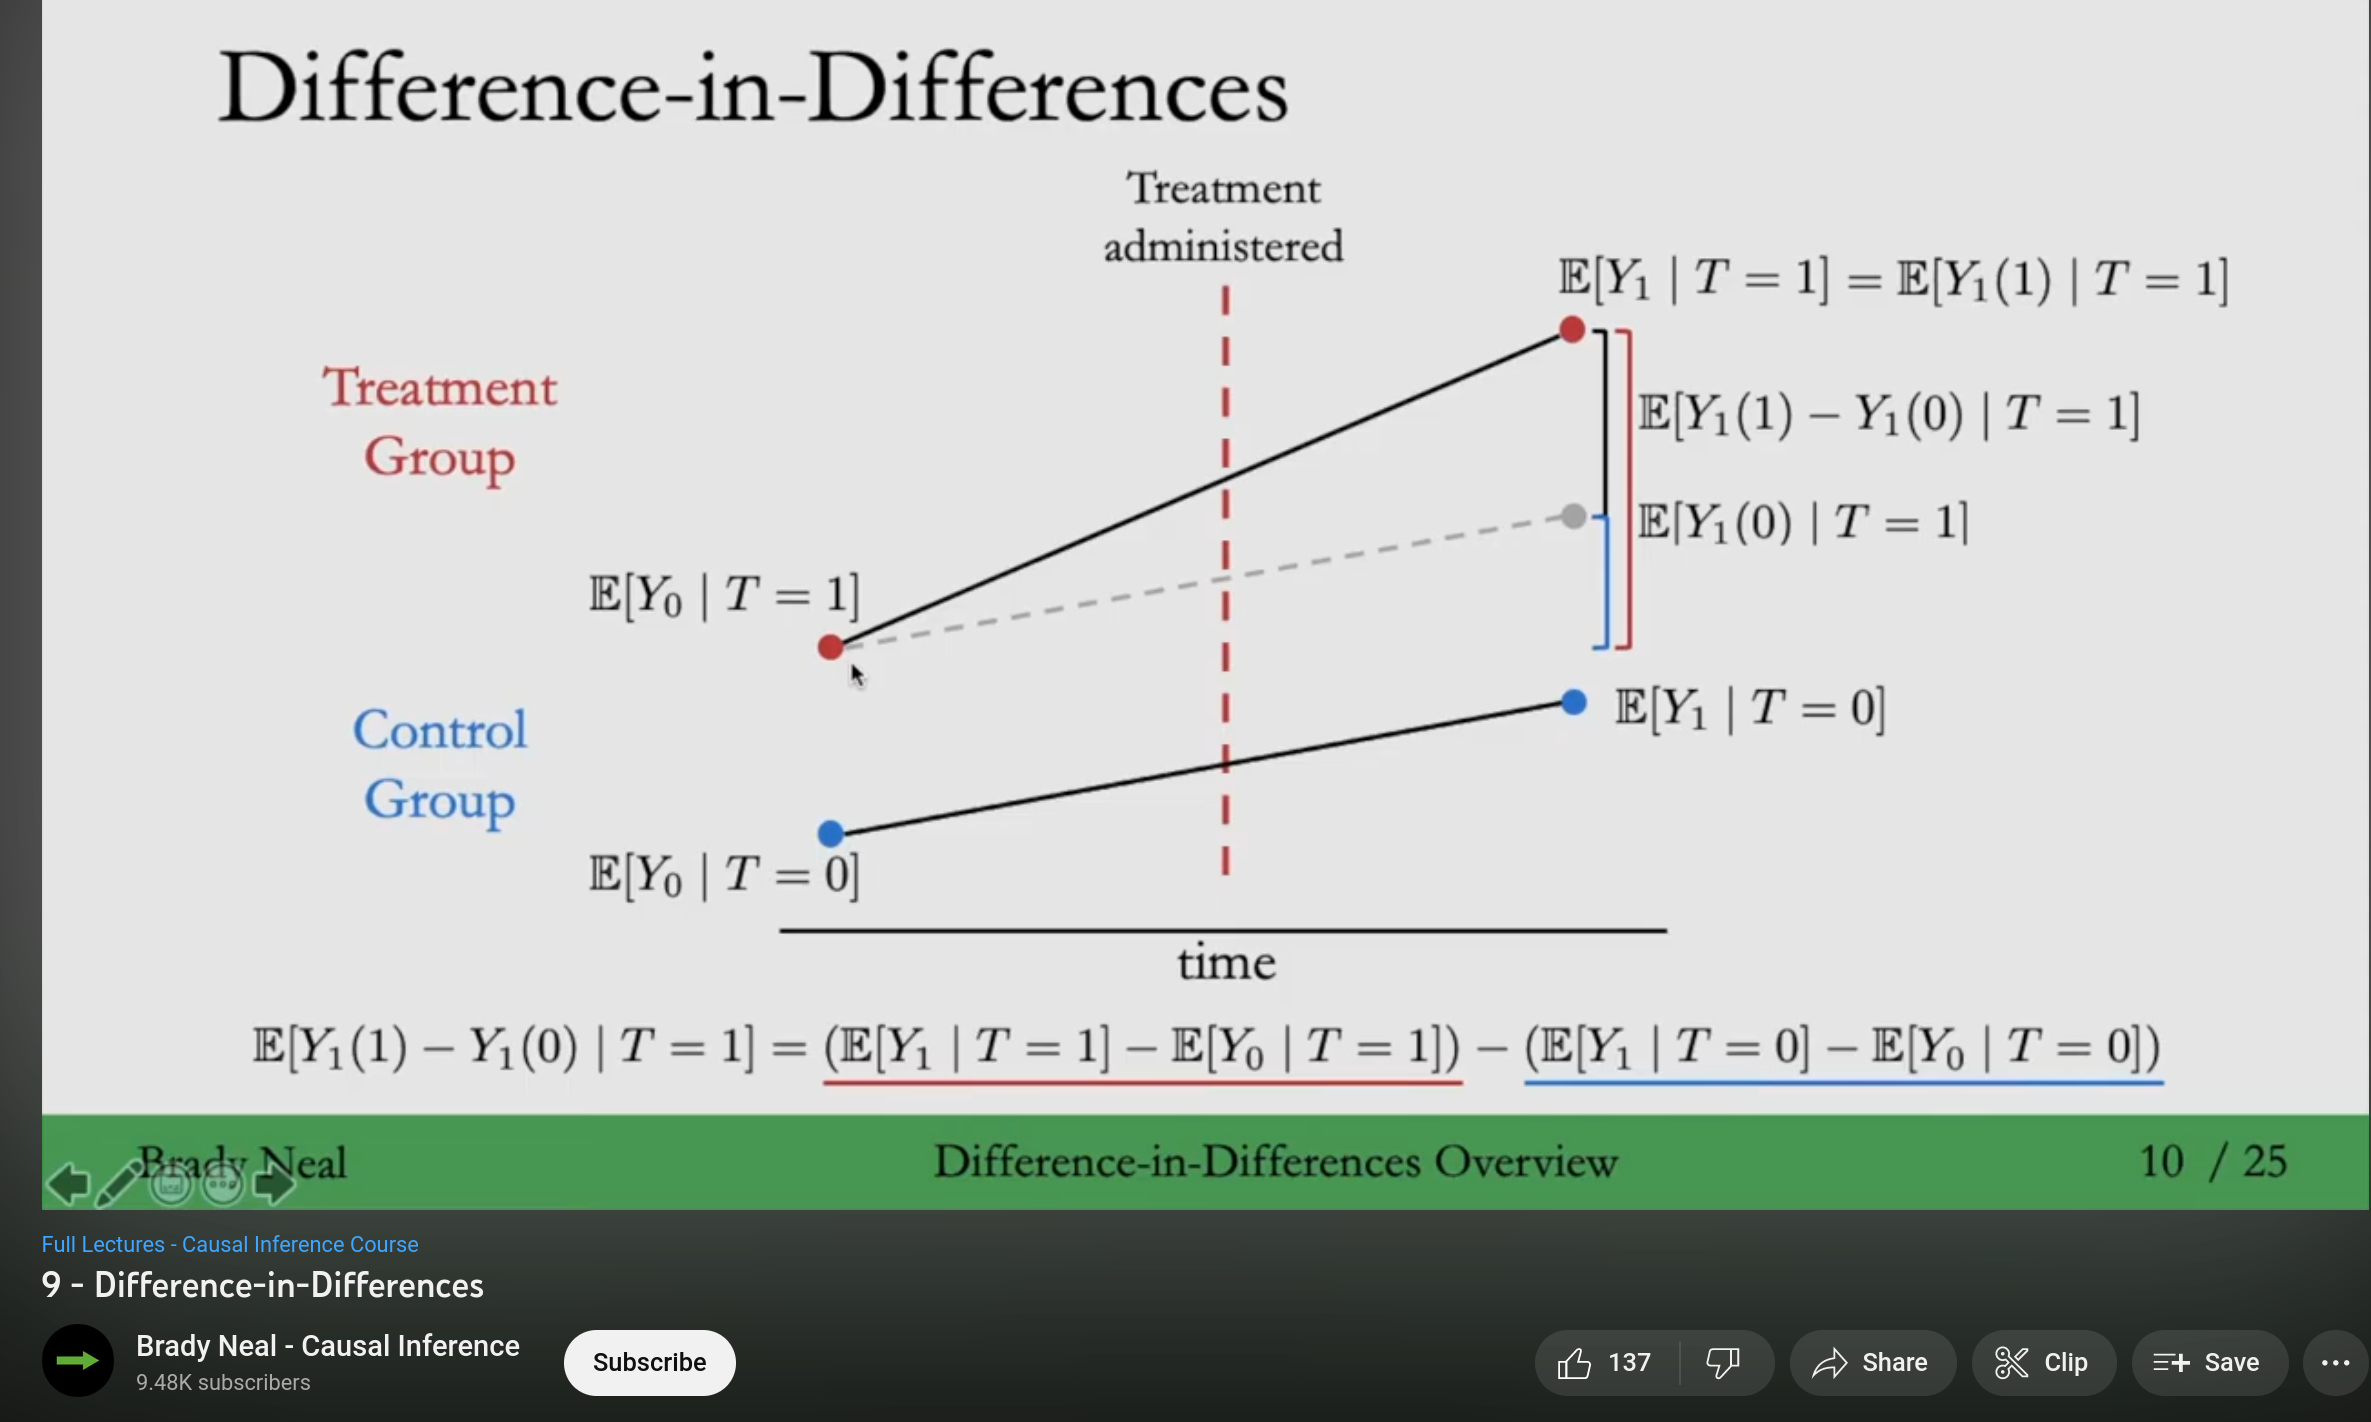
\includegraphics[width=0.9\textwidth,height=\textheight]{fig/neal9.png}
\caption{\label{fig:neal9} Differences-in-Differences}
\end{figure}

\begin{figure}
\centering
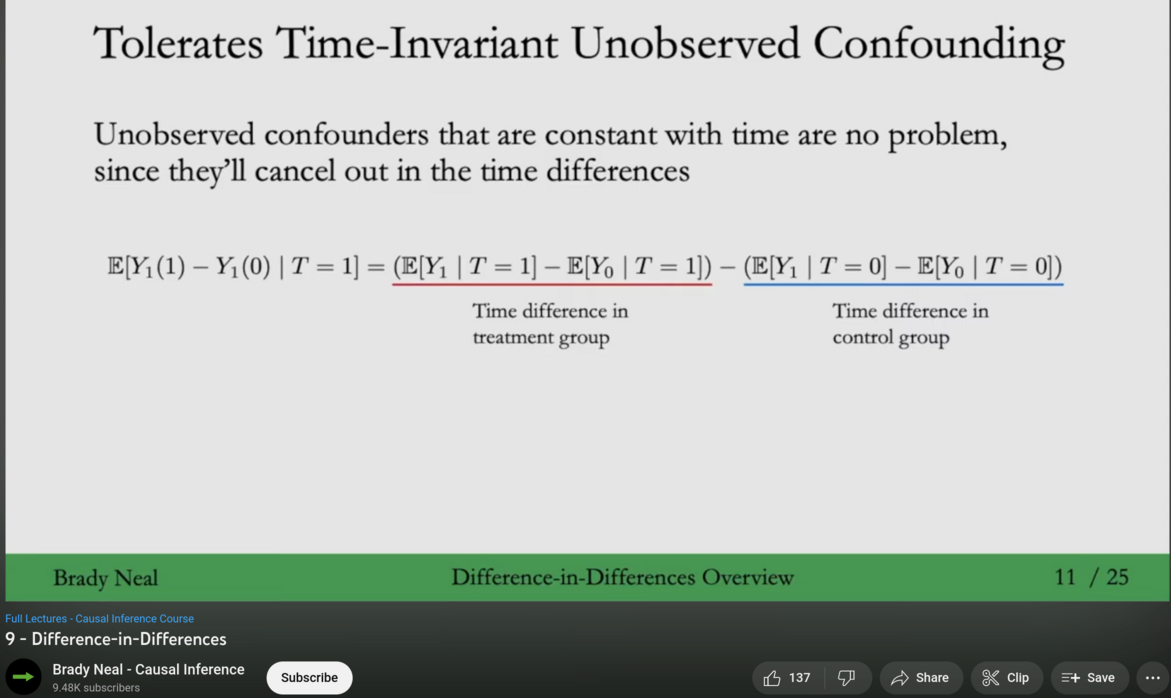
\includegraphics[width=0.9\textwidth,height=\textheight]{fig/neal9b.png}
\caption{\label{fig:neal9b} Tolerate time-invariant unobserved confounding}
\end{figure}

The figures above stem from a video of Brady Neal's lecture on \href{https://youtu.be/2nDgrNP7XSE}{\emph{Difference-in-Differences}}. Please watch this video.

\begin{exercise}
\protect\hypertarget{exr:DiD}{}\label{exr:DiD}Differences-in-Differences

\begin{figure}
\centering
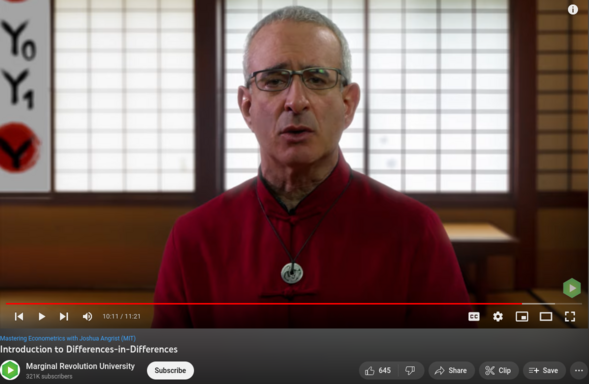
\includegraphics[width=0.5\textwidth,height=\textheight]{fig/angrist-did.png}
\caption[\label{fig:angristdid} Josh Angrist (*1960): Nobel Prize winner of economics in 2021]{\label{fig:angristdid} Josh Angrist (*1960): Nobel Prize winner of economics in 2021\footnotemark{}}
\end{figure}
\footnotetext{The picture stems from the video \url{https://youtu.be/eiffOVbYvNc}}

Watch the video \href{https://youtu.be/eiffOVbYvNc}{\emph{Introduction to Differences-in-Differences}} and answer the following questions. The video is part of a course called \emph{Mastering Econometrics with Joshua Angrist (MIT)} produced by Marginal Revolution University. In it, Josh Angrist introduces differences within differences using one of the worst economic events in history: the Great Depression.

\begin{enumerate}
\def\labelenumi{\arabic{enumi}.}
\tightlist
\item
  In the video, the treatment being examined is:
\end{enumerate}

\begin{enumerate}
\def\labelenumi{\alph{enumi})}
\tightlist
\item
  Bank failure.
\item
  ``Easy'' money.
\item
  ``Tight'' money.
\item
  Differences-in-Differences.
\item
  None of the above.
\end{enumerate}

\begin{enumerate}
\def\labelenumi{\arabic{enumi}.}
\setcounter{enumi}{1}
\tightlist
\item
  If the treatment were effective, which outcome would we expect to observe?
\end{enumerate}

\begin{enumerate}
\def\labelenumi{\alph{enumi})}
\tightlist
\item
  Fewer bank failures.
\item
  Increased bank failures.
\item
  Continued parallel trends.
\item
  No differences in any variables unrelated to bank failure.
\item
  None of the above.
\end{enumerate}

\begin{enumerate}
\def\labelenumi{\arabic{enumi}.}
\setcounter{enumi}{2}
\tightlist
\item
  Practically, how is DD (Differences-in-Differences) typically implemented?
\end{enumerate}

\begin{enumerate}
\def\labelenumi{\alph{enumi}.}
\tightlist
\item
  Non-parametric statistical techniques.
\item
  Randomized trials.
\item
  Regression analysis.
\item
  Instrumental variables.
\item
  None of the above.
\end{enumerate}

Please find solution to the exercise \protect\hyperlink{sol:DiD}{in the appendix.}
\end{exercise}

\hypertarget{appendix}{%
\chapter{Appendix}\label{appendix}}

\hypertarget{sol:effect1u2}{%
\subsection*{Solution to exercise \ref{exr:effect1u2}: The Effect ch.1+2}\label{sol:effect1u2}}

Answers: 1. c), 2. c), 3. a)

\hypertarget{sol:featofresear}{%
\subsection*{Solution to exercise \ref{exr:featofresear}: Features of research}\label{sol:featofresear}}

Answers:

\begin{enumerate}
\def\labelenumi{\arabic{enumi}.}
\tightlist
\item
  a), 2. b), 3. c), 4. d), 5. c), 6. b), 7. c), 8. a), 9. d)
\end{enumerate}

\hypertarget{sol:causalinf1}{%
\subsection*{Solution to exercise \ref{exr:causalinf1}: Causal inference ch.~1}\label{sol:causalinf1}}

Answers:

\begin{enumerate}
\def\labelenumi{\arabic{enumi}.}
\item
  Some common misconceptions about causality that the author addresses in chapter 1 include confusion between correlation and causality, and the belief that observational studies cannot (hardly) establish causality without prior knowledge. He says that human beings ``engaging in optimal behavior are the main reason correlations almost never reveal causal relationships, because rarely are human beings acting randomly'' which is crucial for identifying causal effects.
\item
  The role of randomization in causal inference, as described in the book, is that it helps to control for confounding variables and allows for the estimation of causal effects.
\end{enumerate}

\hypertarget{sol:graduateadmission}{%
\subsection*{Solution to exercise \ref{exr:graduateadmission}: Simpson's Paradox}\label{sol:graduateadmission}}

\begin{enumerate}
\def\labelenumi{\alph{enumi})}
\tightlist
\item
  Assumption 1 is that in any given discipline male and female applicants do not differ in respect of their intelligence, skill, qualifications, promise, or other attribute deemed legitimately pertinent to their acceptance as students. It is precisely this assumption that makes the study of ``sex bias'' meaningful, for if we did not hold it any differences in acceptance of applicants by sex could be attributed to differences in their qualifications, promise as scholars, and so on. (\ldots) Assumption 2 is that the sex ratios of applicants to the various fields of graduate study are not importantly associated with any other factors in admission. \citep[page 398]{Bickel1975Sex}
\item
  Expectations were taken based on the overall acceptance rate of about 0.416 and multiplied by the total observed numbers of applicants admitted and rejected. For example: \((3738+4704) \cdot 0.41666 \approx 3460\) and \((3738+4704) \cdot (1-0.41666) \approx 4981\). Taking the difference of these two measures gives the number to be explained.
\item
  The analogy is explained on page 400:
\end{enumerate}

\begin{quote}
``Picture a fishnet with two different mesh sizes. A school of fish, all of identical size (assumption 1), swim toward the net and seek to pass. The female fish all try to get through the small mesh, while the male fish all try to get through the large mesh. On the other side of the net all the fish are male. Assumption 2 said that the sex of the fish had no relation to the size of the mesh they tried to get through. It is false.''
\end{quote}

The UC Berkley case is just one of many examples to illustrate that uniformity of group assignment of individuals is a necessary condition to ensure that pooling of data does not lead to misleading conclusions when using statistics. The phenomenon of obtaining different results depending on whether one considers the data pooled or unpooled is often referred to as the \emph{Simpson Paradox}.

\hypertarget{sol:simpsonpara}{%
\subsection*{Solution to exercise \ref{exr:simpsonpara}: Simpson's Paradox}\label{sol:simpsonpara}}

Answers:

\begin{enumerate}
\def\labelenumi{\arabic{enumi}.}
\tightlist
\item
  a), 2. c) and d)
\end{enumerate}

\hypertarget{sol:treatmenteffects}{%
\subsection*{Solution to exercise \ref{exr:treatmenteffects}: Treatment effects}\label{sol:treatmenteffects}}

\begin{enumerate}
\def\labelenumi{\arabic{enumi}.}
\tightlist
\item
  The individual treatment effect (ITE) is a measure of the effect of a treatment or intervention on an individual level. It represents the difference in the outcome for an individual who receives the treatment versus the outcome for that same individual if they had not received the treatment.
\item
  The average treatment effect (ATE) is a measure of the difference in the expected outcomes between a treatment group and a control group. It represents the overall effect of a treatment on the population as a whole.
\item
  The ATE is calculated by taking the difference between the average outcome for the treatment group and the average outcome for the control group.
\item
  No, the ATE is a population-level measure and cannot be used to determine the effect of a treatment on an individual level. To determine the effect of a treatment on an individual level, you would need to use techniques such as propensity score matching or instrumental variables.
\item
  Some potential sources of bias when estimating the ATE include selection bias, measurement bias, and unobserved confounding variables. To mitigate these biases, researchers may use randomization or other advanced statistical techniques such as propensity score matching or instrumental variables to control for these potential sources of bias.
\end{enumerate}

\hypertarget{sol:randomsampling}{%
\subsection*{Solution to exercise \ref{exr:randomsampling}: Random sampling}\label{sol:randomsampling}}

Random sampling is a sampling procedure by which each member of a population has an equal
chance of being included in the sample. Random sampling ensures a representative sample. There
are several types of random sampling. In simple random sampling, not only each item in the
population but each sample has an equal probability of being picked. In systematic sampling,
items are selected from the population at uniform intervals of time, order, or space (as in picking
every one-hundredth name from a telephone directory). Systematic sampling can be biased easily,
such as, for example, when the amount of household garbage is measured on Mondays (which
includes the weekend garbage). In stratified and cluster sampling, the population is divided into
strata (such as age groups) and clusters (such as blocks of a city) and then a proportionate
number of elements is picked at random from each stratum and cluster. Stratified sampling is
used when the variations within each stratum are small in relation to the variations between
strata. Cluster sampling is used when the opposite is the case. In what follows, we assume
simple random sampling. Sampling can be from a finite population (as in picking cards from
a deck without replacement) or from an infinite population (as in picking parts produced by a
continuous process or cards from a deck with replacement).

The larger the sample gets the closer we get to the population and hence, we reduce the bias of
having a non-randomly selected sample.

\hypertarget{sol:summarystatistics}{%
\subsection*{Solution to exercise \ref{exr:summarystatistics}: Summary statistics}\label{sol:summarystatistics}}

\begin{longtable}[]{@{}lcc@{}}
\toprule()
Metric & 1 & 2 \\
\midrule()
\endhead
Mode & 21 & 3 \\
Median & 29.5 & 3 \\
P20 & 21 & 2 \\
Range & 71 & 5 \\
IQR & 25 & 1.5 \\
Arithmetic mean & 37 & 3.5 \\
\(\sigma^2\) & 485.33 & 1.5591 \\
\(\sigma\) & 22.030 & 1.248621 \\
COV & 0.5954 & 2.4027 \\
\bottomrule()
\end{longtable}

\hypertarget{sol:guessstat}{%
\subsection*{Solution to exercise \ref{exr:guessstat}: Guess the summary statistics}\label{sol:guessstat}}

\begin{longtable}[]{@{}
  >{\raggedright\arraybackslash}p{(\columnwidth - 10\tabcolsep) * \real{0.1644}}
  >{\centering\arraybackslash}p{(\columnwidth - 10\tabcolsep) * \real{0.1644}}
  >{\centering\arraybackslash}p{(\columnwidth - 10\tabcolsep) * \real{0.1644}}
  >{\centering\arraybackslash}p{(\columnwidth - 10\tabcolsep) * \real{0.1644}}
  >{\centering\arraybackslash}p{(\columnwidth - 10\tabcolsep) * \real{0.1644}}
  >{\centering\arraybackslash}p{(\columnwidth - 10\tabcolsep) * \real{0.1781}}@{}}
\toprule()
\begin{minipage}[b]{\linewidth}\raggedright
varlabel
\end{minipage} & \begin{minipage}[b]{\linewidth}\centering
a
\end{minipage} & \begin{minipage}[b]{\linewidth}\centering
b
\end{minipage} & \begin{minipage}[b]{\linewidth}\centering
c
\end{minipage} & \begin{minipage}[b]{\linewidth}\centering
d
\end{minipage} & \begin{minipage}[b]{\linewidth}\centering
e
\end{minipage} \\
\midrule()
\endhead
Variance & 2 (4.6666) & 4 (466.66) & 5 (800.33) & 1 (4.6666) & 3 (466.66) \\
COV & 1 (.02160) & 3 (.21602) & 5 (.56580) & 4 (.54006) & 2 (.02160) \\
Mean & 3 (100) & 4 (100) & 2 (50) & 1 (4) & 5 (1000) \\
Median & 3 (100) & 4 (100) & 2 (50) & 1 (4) & 5 (1000) \\
Range & 1 (6) & 4 (60) & 5 (98) & 2 (6) & 3 (60) \\
SD & 1 (2.1602) & 4 (21.602) & 5 (28.290) & 2 (2.1602) & 3 (21.602) \\
\bottomrule()
\end{longtable}

\hypertarget{sol:destatexcel}{%
\subsection*{Solution to exercise \ref{exr:destatexcel}: Summary statistics in spreadsheet software}\label{sol:destatexcel}}

\begin{longtable}[]{@{}lc@{}}
\toprule()
Mittelwert & 56 \\
\midrule()
\endhead
Standardfehler & 11,4697670227235 \\
Modus & 0 \\
Median & 55 \\
Erstes Quartil & 42,5 \\
Drittes Quartil & 85 \\
Varianz & 1315,55555555556 \\
Standardabweichung & 36,2705880232945 \\
Kurtosis & -0,731538352420953 \\
Schräge & -0,417051115341008 \\
Bereich & 100 \\
Minimum & 0 \\
Maximum & 100 \\
Summe & 560 \\
Anzahl & 10 \\
\bottomrule()
\end{longtable}

\hypertarget{sol:DiD}{%
\subsection*{Solution to exercise \ref{exr:DiD}: Differences-in-Differences}\label{sol:DiD}}

Answers: 1. b), 2. a), 3. c)

  \bibliography{book.bib}

\end{document}
